\documentclass[a4paper]{article}
\usepackage[brazilian]{babel}
\usepackage[utf8]{inputenc}
\usepackage{graphicx}
\usepackage{caption}
\usepackage{indentfirst}
\usepackage{float}
\usepackage{setspace}
\usepackage{fancyhdr}
\usepackage{amssymb}
\usepackage{amsmath}
\usepackage{amsfonts,amssymb}
\usepackage{hyperref}
\usepackage{color}
\usepackage{multirow}
\usepackage{booktabs}
\usepackage{listings}
\usepackage[top=2cm,left=2.85cm,right=2.85cm,bottom=2.6cm]{geometry}
\newcommand{\HRule}{\rule{\linewidth}{0.5mm}}
\renewcommand{\baselinestretch}{1.2}
\setlength{\parskip}{0.5\baselineskip}
\captionsetup[figure]{labelfont={bf},name={Fig.},labelsep=period}
\usepackage{subfig}
\usepackage{listings}
\usepackage{xcolor}
\lstset{
    columns=fixed,       
    numbers=left,                                        % 在左侧显示行号
    frame=none,                                          % 不显示背景边框
    backgroundcolor=\color[RGB]{255,255,255},            % 设定背景颜色
    keywordstyle=\color[RGB]{40,40,255},                 % 设定关键字颜色
    numberstyle=\footnotesize\color{darkgray},           % 设定行号格式
    commentstyle=\it\color[RGB]{0,96,96},                % 设置代码注释的格式
    stringstyle=\rmfamily\slshape\color[RGB]{128,0,0},   % 设置字符串格式
    showstringspaces=false,                              % 不显示字符串中的空格
    language=python,                                        % 设置语言
}

\begin{document}
\vspace{6mm}
\begin{center}
\Huge\textbf{Aerial Cactus Identification}
\end{center}
\vspace{3mm}

\begin{figure}[h]
\centering

\includegraphics[width=8cm,height=8cm]{sysu.png}
\end{figure}

\begin{center}
\large\textbf{16340154 --  Shuo Liu }\\
\end{center}

\begin{center}
\normalsize{School of Data and Computer Science, Sun Yat-sen University}
\end{center}

\begin{center}
\textit{July. $10^{nd}$ \textit, 2019\\}
\end{center}
\vspace{6mm}

\begin{figure}[H]
\centering
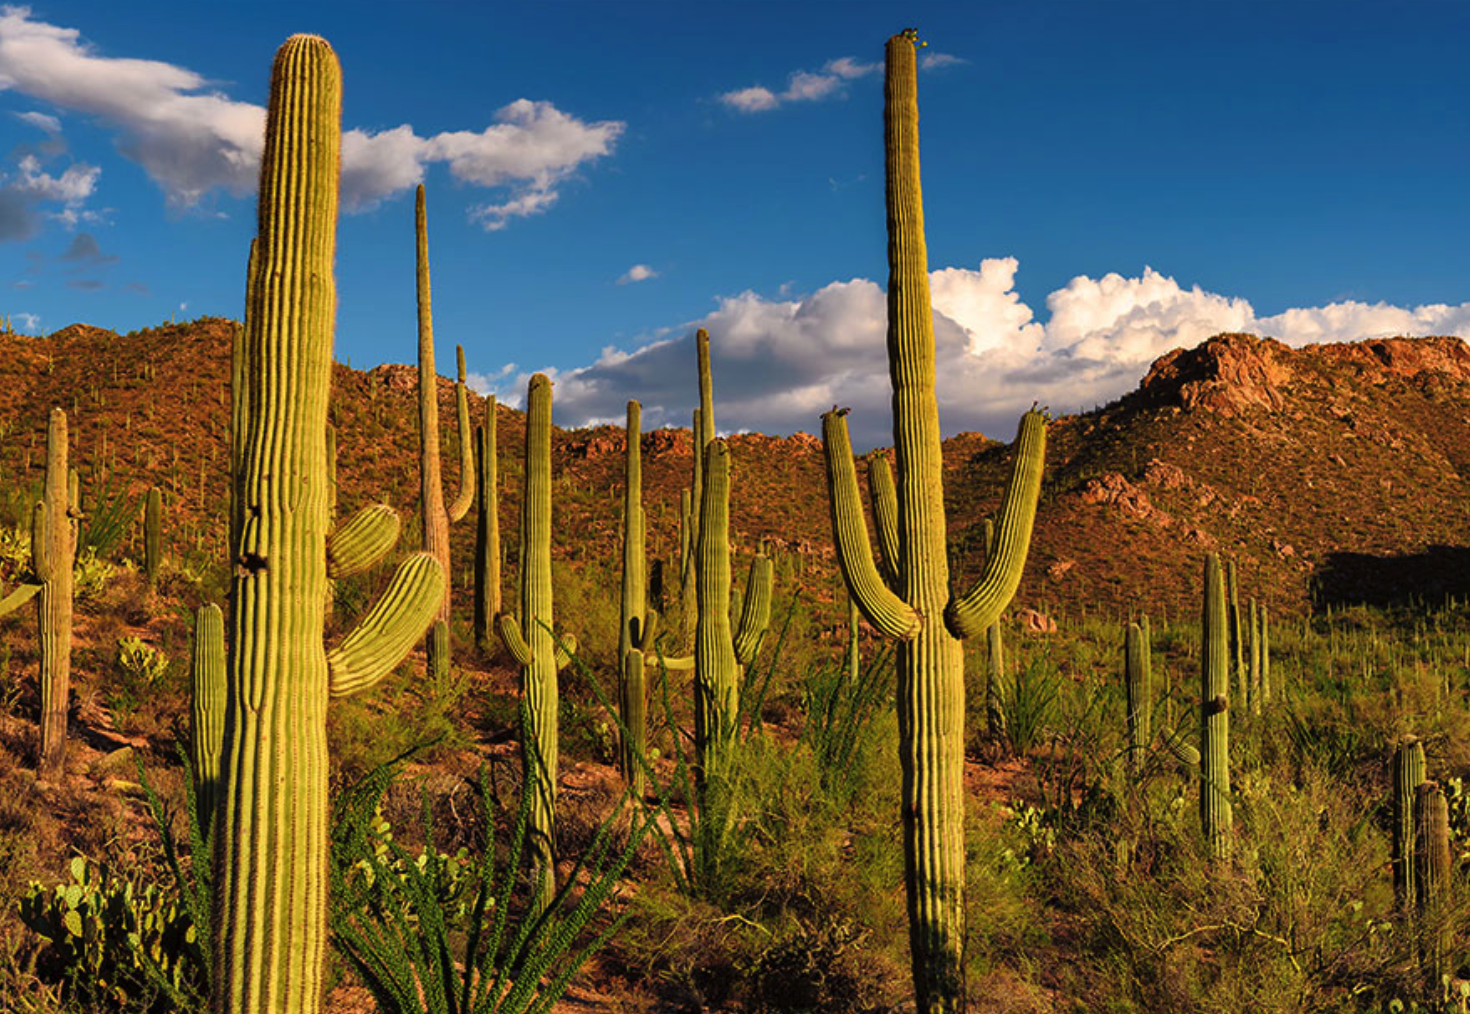
\includegraphics[width=15cm,height=10cm]{cactus.png}
\end{figure}
\clearpage

\noindent \HRule
\vspace{2.5mm} \\
\large{\textbf{Summary. }\emph{In order to recognize the vegetation inside the protected areas of Mexico, we aim to build models to identify a specific type of cactus from UAVs. In this scientific report, five architectures (\textsf{VGGNet}, \textsf{ResNet}, \textsf{SEResNet}, \textsf{DenseNet}, \textsf{ResNeXt}) are well-designed for \href{https://www.kaggle.com/c/aerial-cactus-identification}{Kaggle competition: \texttt{Aerial Cactus Identification}}. Within each architecture, we build three distinct models (\textit{except for \textsf{ResNeXt}}). Evaluations are made between different models and architectures. Additionally, experimental results help us to find the most suitable parameters. Moreover, we find that property differences exist in different architectures, and the \textsf{DenseNet-161} model has the best performance. \\ }}
\vspace{2mm}
\HRule

%%
\vspace{6mm}
\begin{center}
\LARGE\textbf{I. Introduction} \\
\end{center}
\vspace{2mm}

\large{\noindent To assess the impact of climate change on Earth's flora and fauna, it is vital to quantify how human activities such as logging, mining, and agriculture are impacting our protected natural areas. Researchers in Mexico have created the \href{https://jivg.org/research-projects/vigia/}{VIGIA project}, which aims to build a system for autonomous surveillance of protected areas. A first step in such an effort is the ability to recognize the vegetation inside the protected areas. We are tasked with creation of a model that can identify a specific type of cactus in aerial imagery. The competition information is shown in \textbf{Appendix. A.}

\begin{figure}[h]
\centering
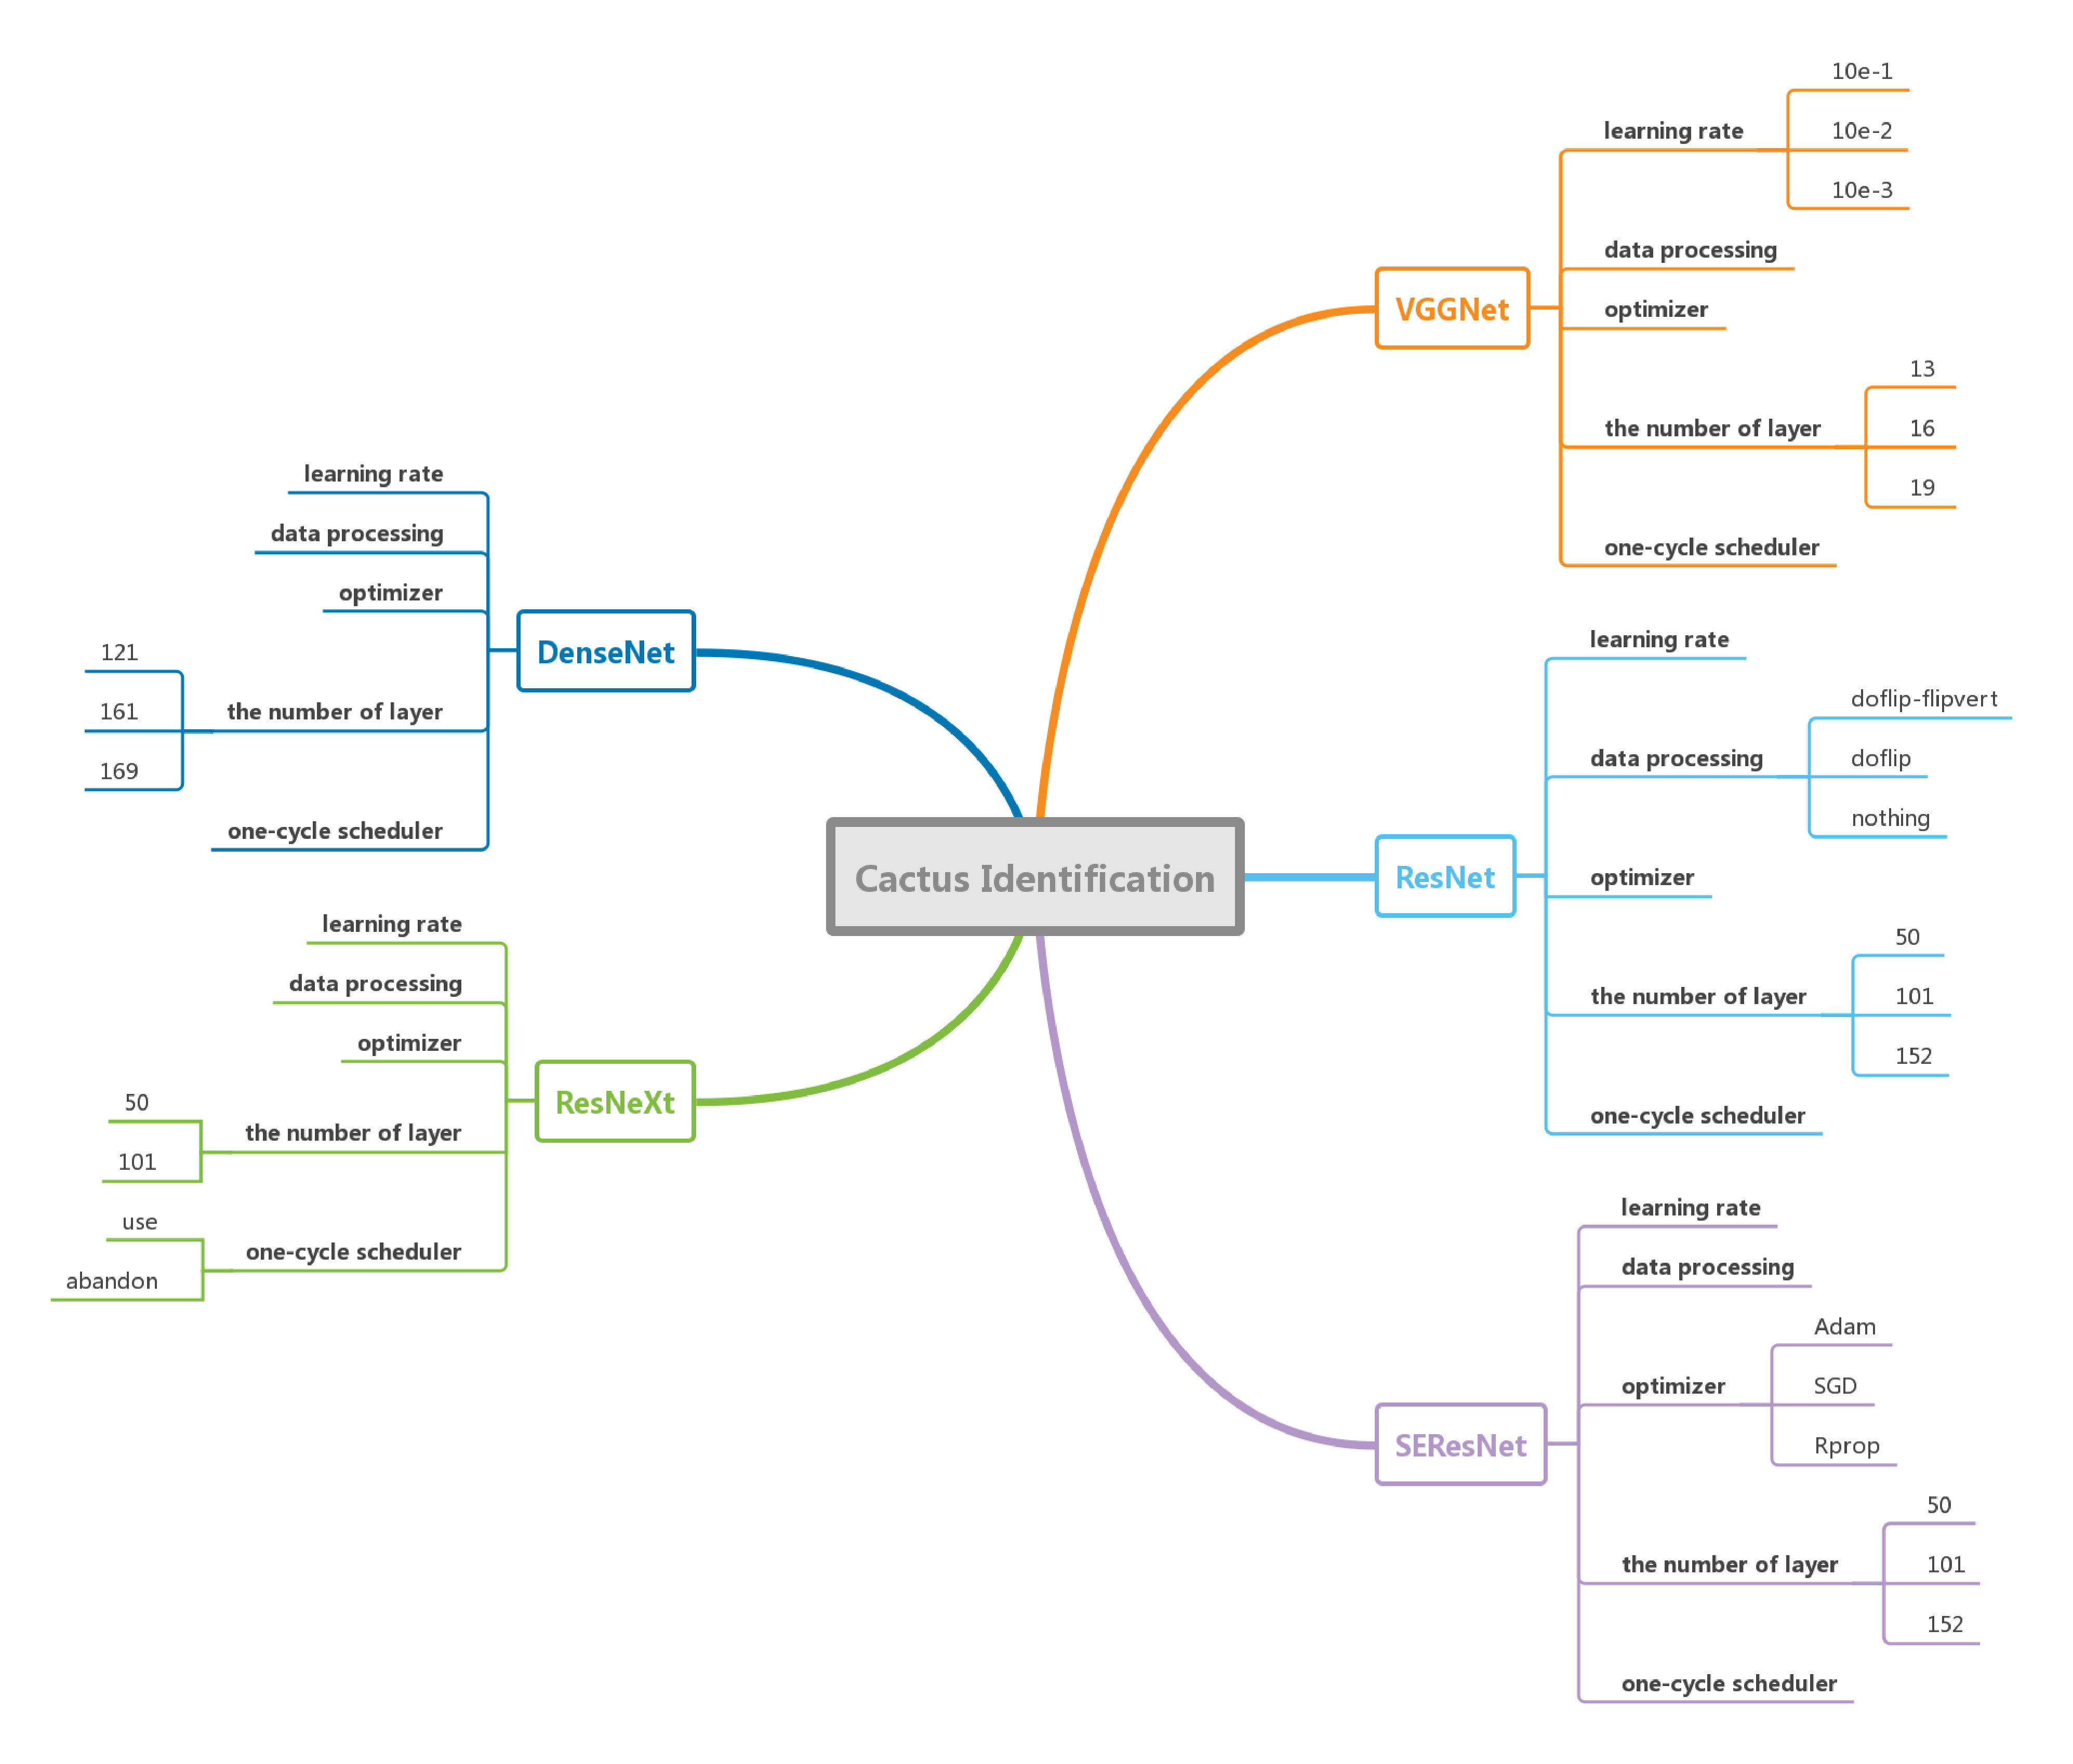
\includegraphics[width=15cm]{overview.pdf}
\caption{Overview of our architectures, models, and parameter settings.}
\label{overview}
\end{figure}

To address this challenge, we use \textbf{5} architectures to deal with the columnar cacti detection and try various settings as shown in \textbf{Fig. \ref{overview}}. By this way, we can evaluate the performance of an architecture as a whole. The architectures we used in the competition are listed as follows:

\begin{itemize}
    \item \href{https://arxiv.org/pdf/1409.1556.pdf}{\textbf{VGGNet}}: \textsf{VGGNet} is a deep convolutional neural network proposed by Visual Geometry Group. It's proved that \textsf{VGGNet} has good results on the prior-art configurations and it also generalizes well to other datasets. Here, we build \textsf{VGGNet-13}, \textsf{VGGNet-16}, and \textsf{VGGNet-19} models in this framework.
    
    \item \href{https://arxiv.org/pdf/1512.03385.pdf}{\textbf{ResNet}}: \textsf{ResNet} is a deep convolutional neural network proposed by He et.$\ $al., whose structure can accelerate the training of neural network very quickly, and the accuracy of the model has been greatly improved. Here, we build \textsf{ResNet-50}, \textsf{ResNet-101}, and \textsf{ResNet-152} models in this framework.
    
    \item \href{https://arxiv.org/pdf/1709.01507.pdf}{\textbf{SEResNet}:} \textsf{SEResNet} is a deep convolutional neural network proposed by Hu et.$\ $al., which focuses on the channel relationship and adds the ``Squeeze-and-Excitation'' (SE) block. Here, we build \textsf{SEResNet-50}, \textsf{SEResNet-101}, and \textsf{SEResNet-152} models in this framework.
    
    \item \href{https://arxiv.org/pdf/1608.06993.pdf}{\textbf{DenseNet}: } Huang et.$\ $al. introduced the Densely Connected Convolutional Network (\textsf{DenseNet}), which connects each layer to every other layer in a feed-forward fashion. Here, we build \textsf{DenseNet-121}, \textsf{DenseNet-161}, and \textsf{DenseNet-169} models in this framework.
    
    \item \href{https://arxiv.org/pdf/1611.05431.pdf}{\textbf{ResNeXt}: }  \textsf{ResNeXt} is an enhancement of \textsf{ResNet} proposed by Xie et.$\ $al., which is constructed by repeating a building block that aggregates a set of transformations with the same topology. Here, we build \textsf{ResNeXt-50} and \textsf{ResNeXt-101} models in this framework.
\end{itemize}

Our contribution is mainly three-fold:

\begin{enumerate}
    \item First, we build try \textbf{5} architectures to deal with the columnar cacti detection. Experimental results show that, with appropriate parameter setting, \textsf{DenseNet-161} model can reach over \textbf{98\%} in this competition.
    \item Second, we deep into these architectures and try \textbf{14} models to evaluate the average performance of them. By this way, we have a more comprehensive insight of each architectures.
    \item Moreover, we try about \textbf{70} parameter settings and compare their outcomes. We get the their best parameter combination. Experimental results show that the impacts of parameters are even larger than those of models and architectures.
\end{enumerate}

The rest of this report is organized as follows. We examplify several popular kernels in this competition and pinpoint their drawbacks in \textbf{Section. II}. We have brief descriptions of five architectures and show their implementation respectively from \textbf{Section. III} to \textbf{Section. VII}. In \textbf{Section. VIII}, we make comparisons of these architectures and show the impacts of parameters on the final score. We make an acknowledgement to the assistant people before making a conclusion in \textbf{Section. IX}.

}

%%
\vspace{5mm}
\begin{center}
\LARGE\textbf{II. Related Work} \\
\end{center}
\vspace{2mm}

Many kernels based on CNN are submitted to make the testing set score higher, including \href{https://www.kaggle.com/ateplyuk/keras-transfer-vgg16}{\textsf{VGGNet-16} by Alexander}, \href{https://www.kaggle.com/ateplyuk/keras-transfer-densenet121}{\textsf{ResNet-34} by Benjamin}, and \href{https://www.kaggle.com/artgor/detecting-cactus-with-kekas}{\textsf{DenseNet-169} by Andrew}. These popular kernels provide us many inspirations when we are solving cactus identification puzzles.

However, none of these work makes a comparison of different parameter settings, (e.g. the learning rate, data pre-processing, optimizer, the number of layer, and scheduler) in the architecture. Thus, we can not clearly see the marginal utility of each measurement. Besides, judging the performance of a specific architectures only by its best score (\textit{i.e., the best parameter combination}) is not rational, as we can not evaluate the average grade of each architecture. 

%%%%% section III. Very deep cnn
\clearpage
\vspace{5mm}
\begin{center}
\LARGE\textbf{III. Very Deep Convolutional Network} \\
\end{center}
\vspace{2mm}

\large{You are able to see our kernel submission page in \textbf{Appendix. B.}}

\vspace{2mm}
\begin{center}
\large\textbf{Architecture} \\
\end{center}


\large{
After trials and errors, our first architecture comes to \textsf{VGGNet}. Here, we build \textsf{VGGNet-13}, \textsf{VGGNet-16}, and \textsf{VGGNet-19} models in this framework.

\textsf{VGGNet} was the second runner-up in the \texttt{2014 ILSVRC competition}, and the first runner-up was \textsf{GoogLeNet}. However, it outperforms \textsf{GoogLeNet} in multiple migration learning tasks. \textsf{VGGNet} is the preferred algorithm for extracting CNN features from images. But it also has drawback that its parameters is about 140M, which requires large storage space.

\begin{figure}[h]
\centering
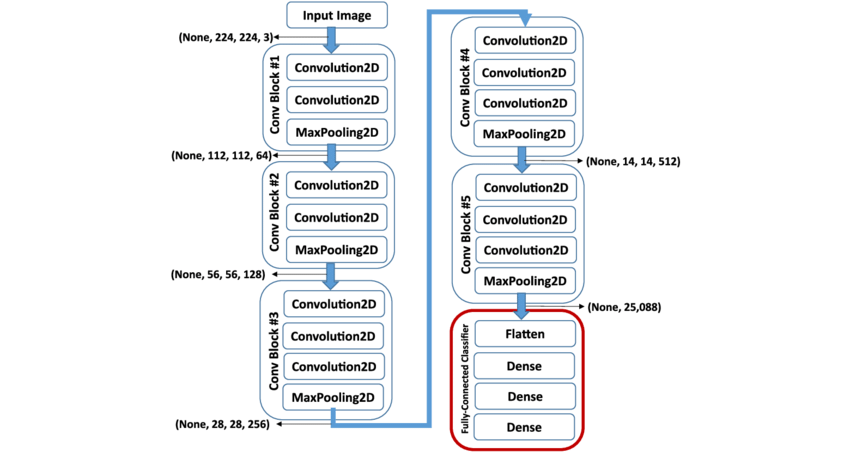
\includegraphics[width=15cm,height=9cm]{A-schematic-of-the-VGG-16-Deep-Convolutional-Neural-Network-DCNN-architecture-trained.png}
\caption{\textsf{VGGNet-16}: An example of deep convolutional neural network.}
\label{vgg16}
\end{figure}

Our network structure is very neat, and there are not much super parameters. Focusing on the construction of a simple network, convolution layers are all followed by a pool layer which can compress the images. The framework of a demo \textsf{VGGNet-16} model is shown in \textbf{Fig. \ref{vgg16}.} 

}

%%%%%
\vspace{2mm}
\begin{center}
\large\textbf{Implementation} \\
\end{center}

\large{

To implement \textsf{VGGNet},we use Conv2d, BatchNorm2d and Relu as basic block, with all Conv2d layers using kernel size of (3,3), stride of (1,1) and padding of (1,1). Blocks are connected sequentially to form the body of model. For pooling, we use MaxPool2d of kernel size of (2,2) and stride of (2,2). 

The head of model uses two AdaptiveAvgPool2d layers to transform the output feature map of body to size [1024, 1, 1], and two linear layers (with out\_features of 512 and 2) to output score for each class. Batch normalization and dropout are used in head of model to avoid over fitting.

Each model is pre-trained. In addition, fine tunning method is used when training, with only parameters of BatchNorm layers and Linear layers trainable. For example, our \textsf{VGGNet-16} has 15252034 parameters in total. However, by fine tunning, only 537346 parameters are trainable. This is very efficient to train the model with good performance.

The loss and accurate curve on the given training set is shown in \textbf{Fig. \ref{vggacc}}. Note that the loss is decreased and the accuracy is improved with the training.

\begin{figure}[h]
\centering
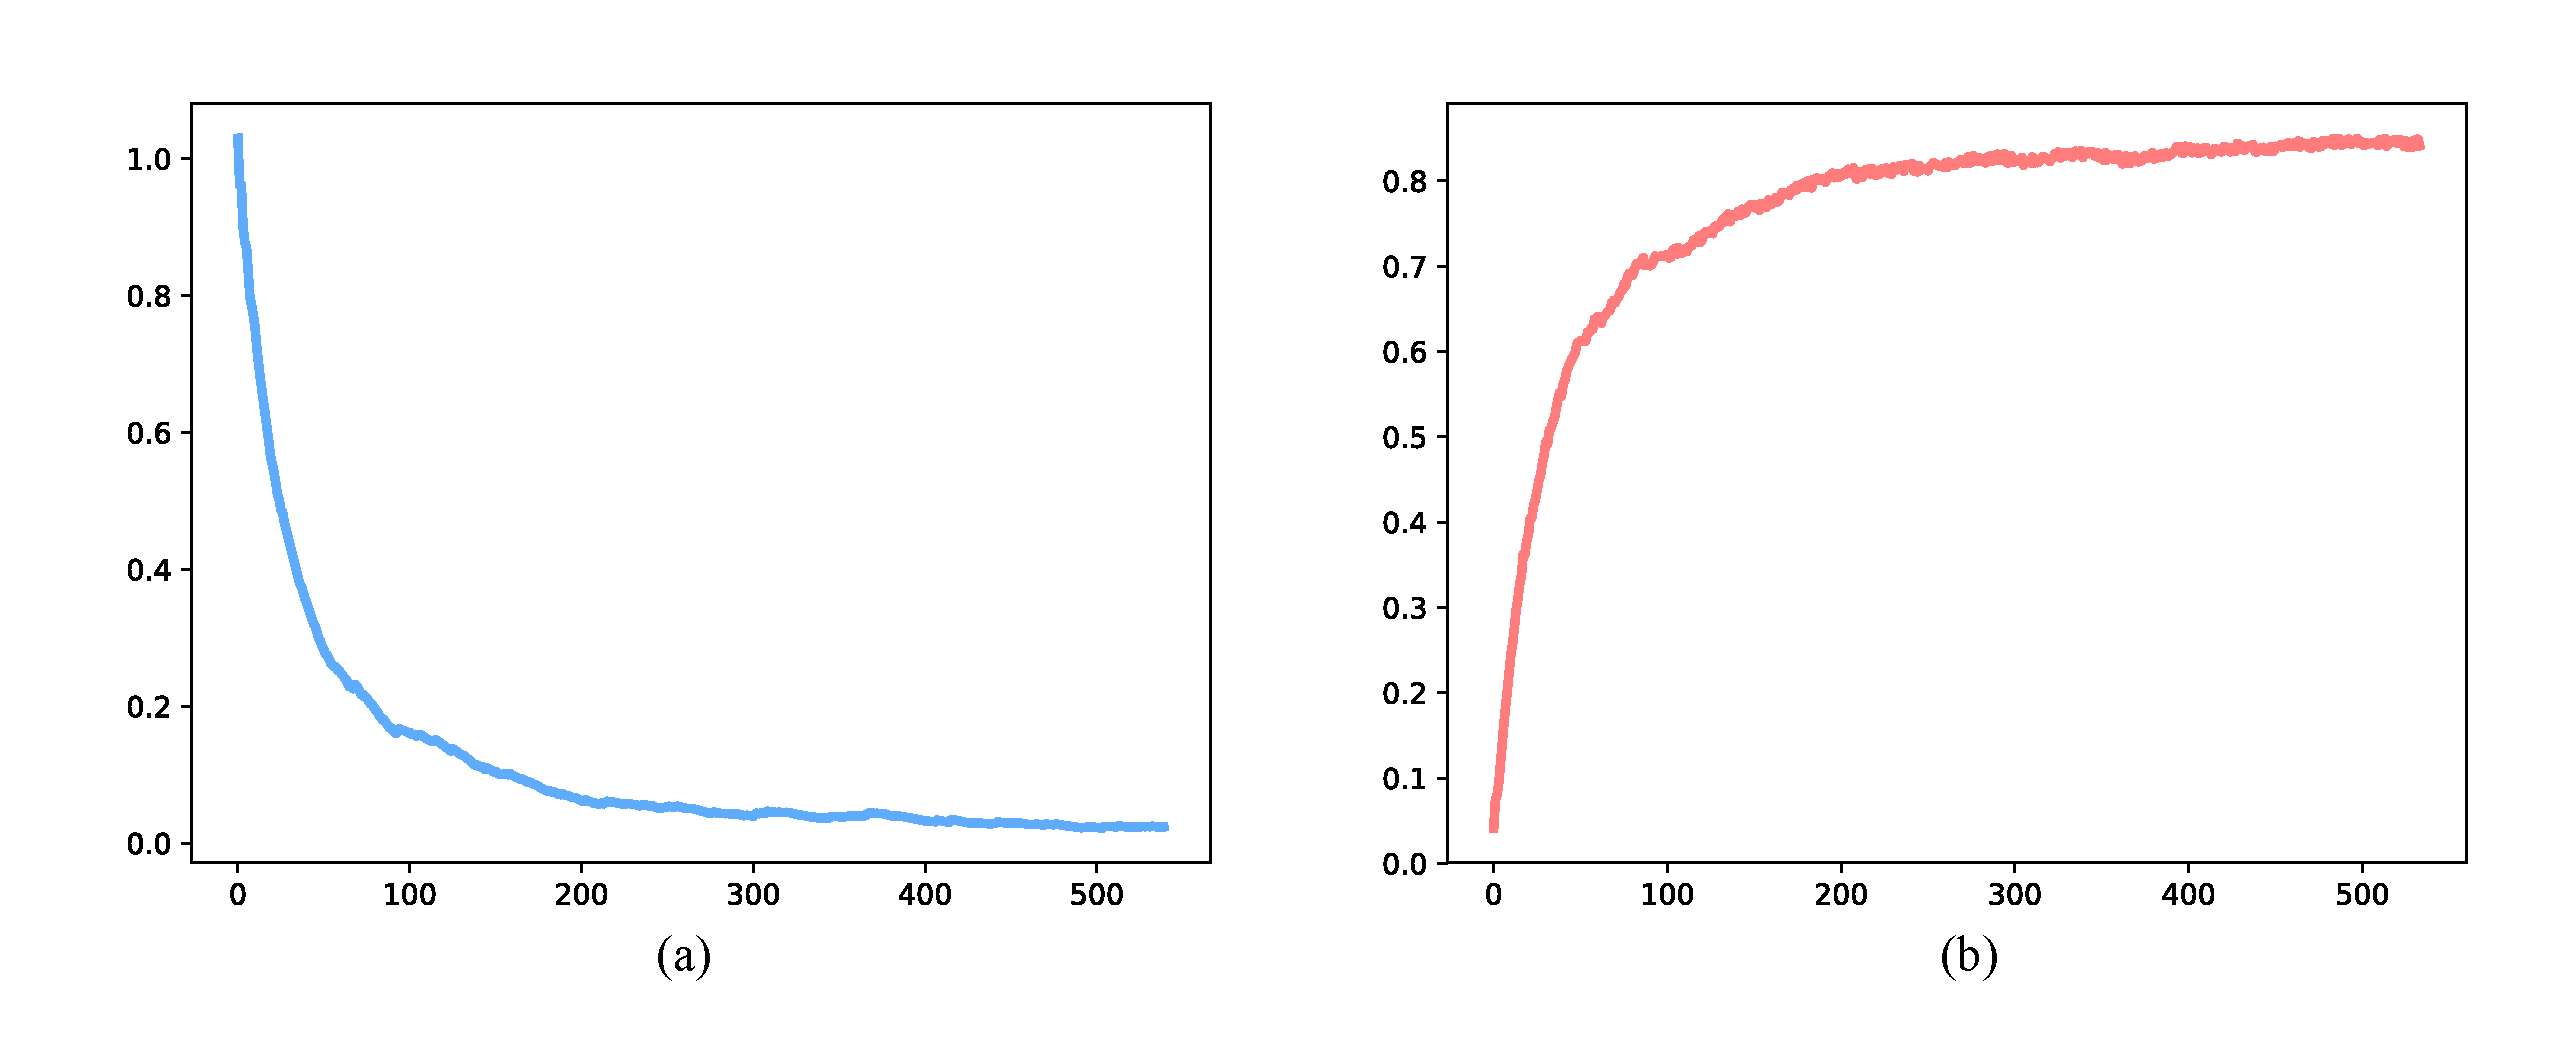
\includegraphics[width=15cm]{vgg_acc.pdf}
\caption{(a): Loss and (b): accuracy curve of \textsf{VGGNet} during the training process.}
\label{vggacc}
\end{figure}

}

\large{You are able to see the source code of this architecture in \textbf{Appendix. C.}}
%%%%%
\vspace{2mm}
\begin{center}
\large\textbf{Results} \\
\end{center}

\large{

\textbf{Fig. \ref{vggresults}} shows the scatter plot of predicted values for 4000 samples and the histogram of predicted values for them. We find that most scatters lie in the scale of 0.0-0.2, meaning that columnar cactus are absent in most images taken by UAVs in the testing set. Plus, most answers are explicit (\textit{i.$\ $e.}, the results are relatively sured), for almost all scatters are distributed in 0-0.2 and 0.8-1 (\textit{i.$\ $e.}, high confidence intervals).

}

\begin{figure}[h]
\centering
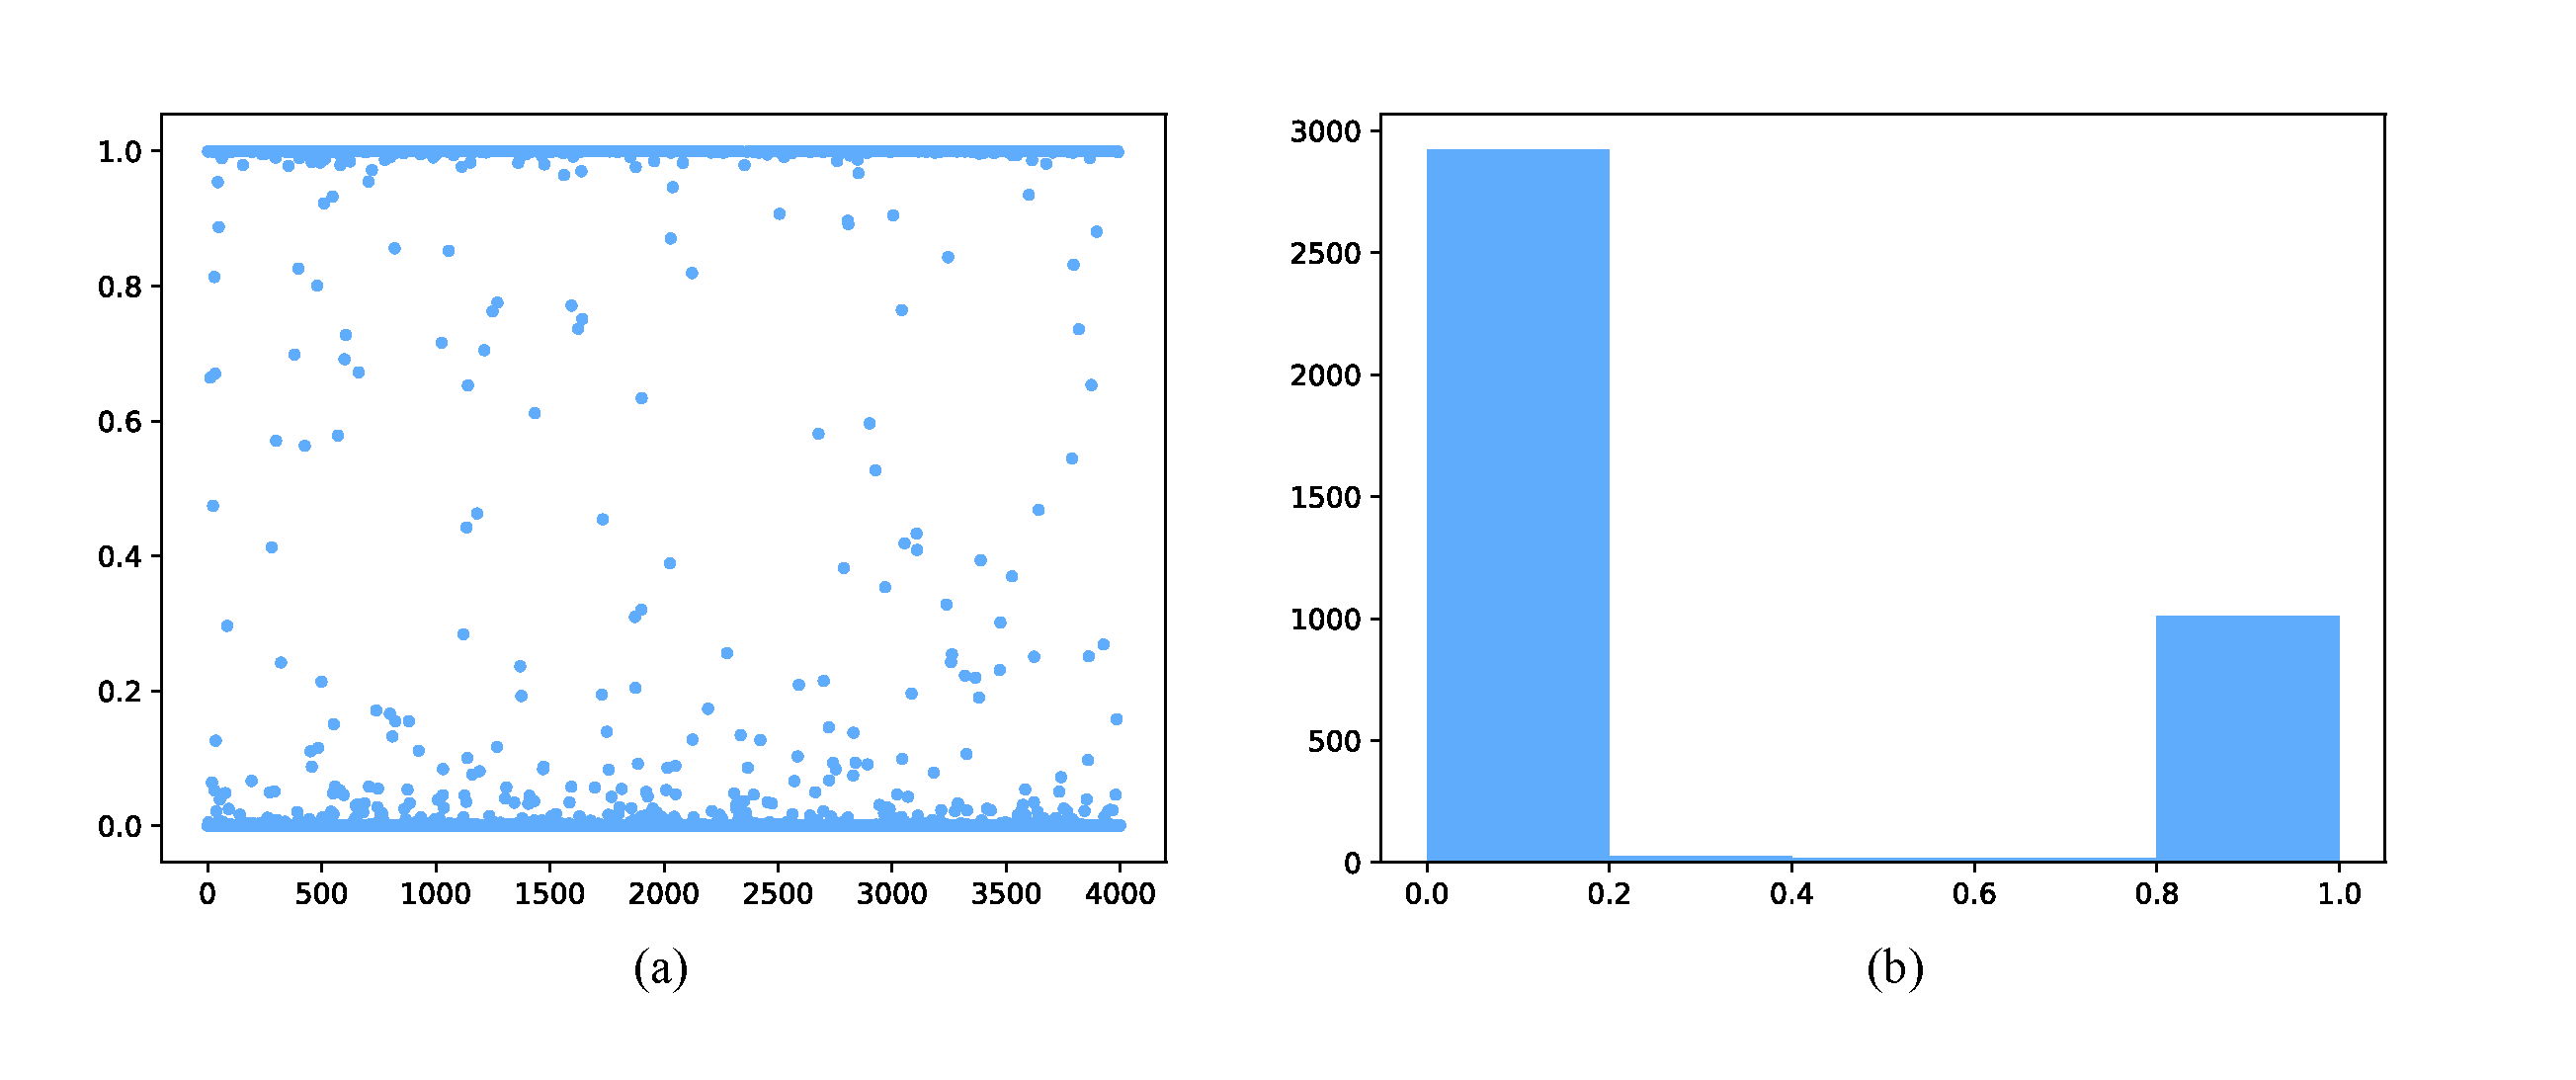
\includegraphics[width=15cm,height=6cm]{vgg_best.pdf}
\caption{ (a): Prediction scatter and (b): prediction histogram of \textsf{VGGNet}.}
\label{vggresults}
\end{figure}

%%%%%
\vspace{2mm}
\begin{center}
\large\textbf{Evaluation} \\
\end{center}

%vgg_16_bn_1e-2_sgd_use-one-cycle_dofilp-flipvert
\large{
Our \textsf{VGGNet} architecture has a up to \textbf{95.85\%} accuracy on the testing set when adopting the appropriate setting, (\textit{i.$\ $e.} 13\_bn layer, 1e-1 learning rate, Adam optimizer, use one-cycle, and do nothing pre-processing). We also compare the impacts of parameters on the final score between different models as shown in \textbf{Fig. \ref{vggcompare}}. We find that pre-processing techniques like flipping images can not make the models more accurate, on the contrary, they even degrade the performance. Among the three models, \textsf{VGGNet-13} perform the best and it's a rational measurement to exploit Adam optimizer in the models. Meanwhile, learning rate of 1e-1 is appropriate for training. The last sub-figure shows that one-cycle scheduler doesn't have huge effect on the overall performance. Note that all of the comparison is base on this baseline -- adopting flip techniques on \textsf{VGGNet-16} with a learning rate of 1e-2, using SGD optimizer and one-cycle scheduler.

\begin{figure}[h]
\centering
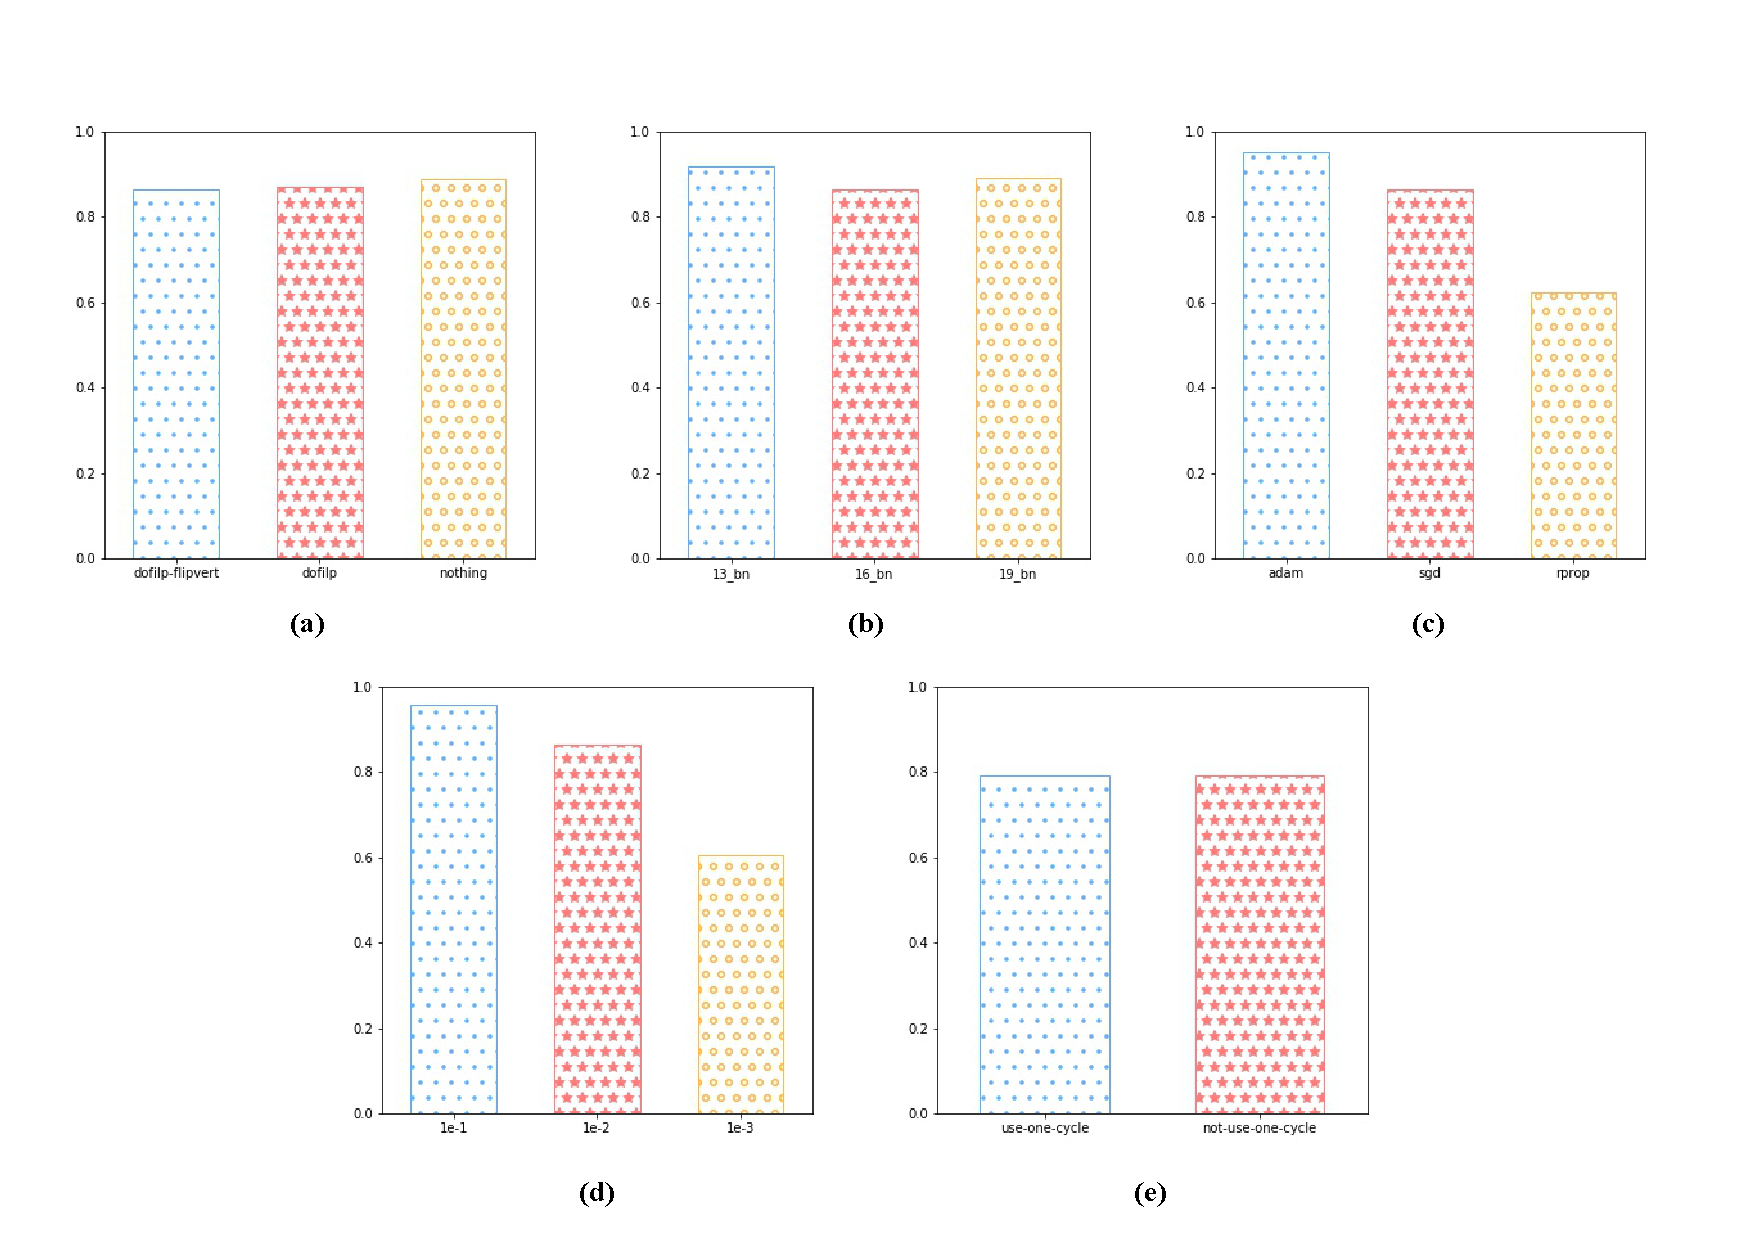
\includegraphics[width=15cm]{vgg.pdf}
\caption{ Impacts of (a): pre-processing techniques, (b): the number of layer, (c): optimizer, (d) learning rate, and (e) scheduler between different models of \textsf{VGGNet}.}
\label{vggcompare}
\end{figure}
}


%%% section IV. Residual Neural Network
\clearpage
\vspace{5mm}
\begin{center}
\LARGE\textbf{IV. Residual Neural Network} \\
\end{center}
\vspace{2mm}

\large{You are able to see our kernel submission page in \textbf{Appendix. B.}}

\vspace{2mm}
\begin{center}
\large\textbf{Architecture} \\
\end{center}


\large{
After trials and errors, we select \textsf{ResNet} as our second architecture. Here, we build \textsf{ResNet-50}, \textsf{ResNet-101}, and \textsf{ResNet-152} models in this framework. 

Based on \textsf{VGGNet}, \textsf{ResNet} inserts shortcut connections, which turns the network into its counterpart residual version. The identity shortcuts can be directly used when the input and output are of the same dimensions. 

In the structure of \textsf{ResNet}, two residual modules could be used, one is the concatenation of two 3*3 convolution networks as a residual module, and the other is the concatenation of 3 convolution networks as a residual module, as shown in \textbf{Fig. \ref{resblock}(a), (b)}. Embedding of the residual block works as follows in \textbf{Fig. \ref{resblock}(c)}. ``Global pooling'' refers to the changing from input c*h*w to output c*1*1 for pooling layer; ``FC'' refers to the full connection layer; ``ReLU'' is used as the activation function between the two full connection layers; after passing the two full connection layers, the activation function -- sigmoid -- is used to activate; finally, the values obtained are multiplied by the original input to get the output. 

\begin{figure}[h]
\centering
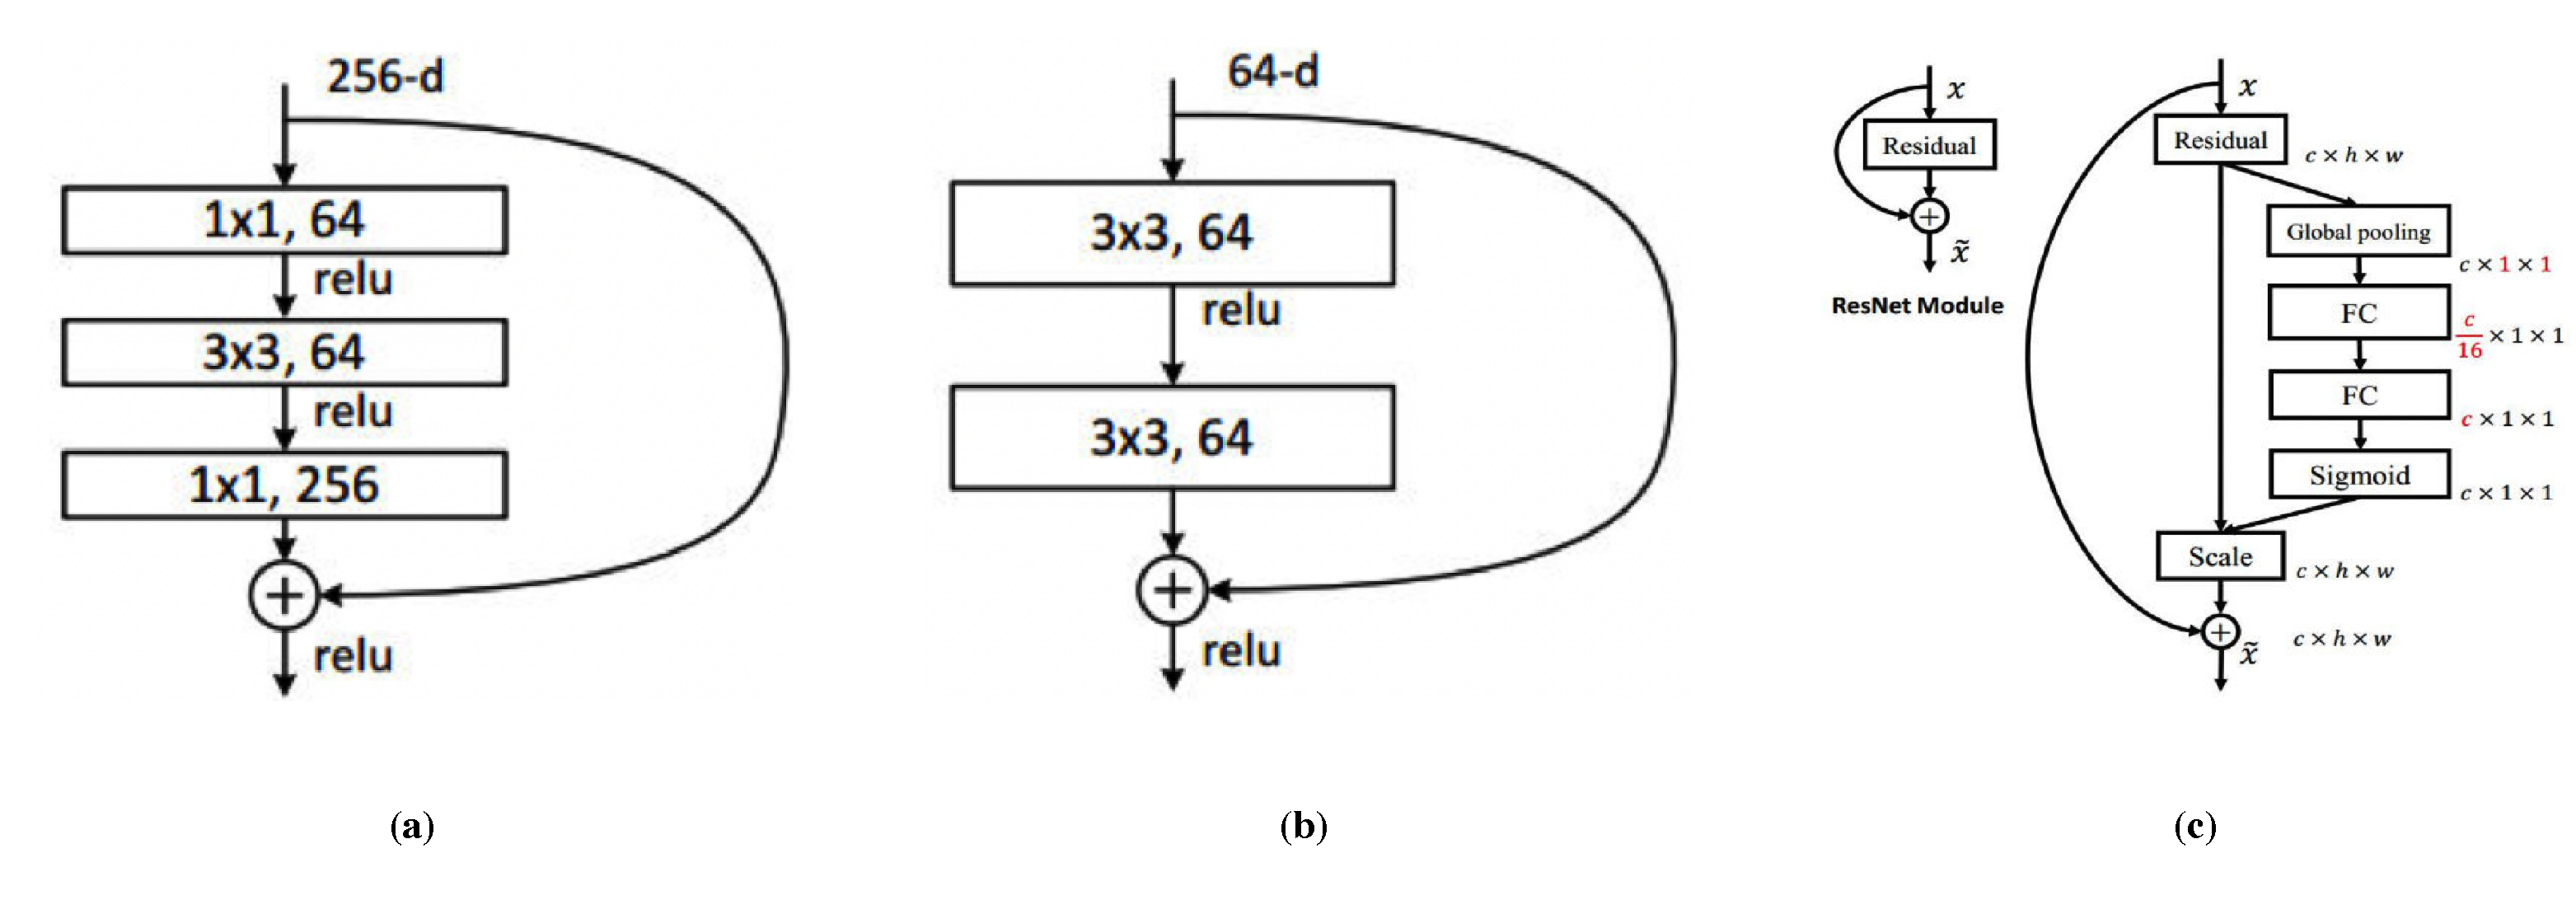
\includegraphics[width=15cm]{resblock.pdf}
\caption{ (a), (b): Two kinds of residual block of \textsf{ResNet} and (c): the embedding of residual block.}
\label{resblock}
\end{figure}

}

%%%%%
\vspace{2mm}
\begin{center}
\large\textbf{Implementation} \\
\end{center}

\large{

To implement \textsf{ResNet},we use structure of Bottleneck to construct basic blocks  consist of three Conv2d layers, three BatchNorm2d layers and Relu as the output function for each block. Conv2d layers in each bottleneck block use small kernel size of (3,3) and (1,1). Bottleneck blocks are connected sequentially to form the body of model. As for pooling, we use MaxPool2d of kernel size of (3,3) and stride of (2,2). 

The head of model uses two AdaptiveAvgPool2d layers to transform the output feature map of body to size [4096, 1, 1], and two linear layers (with out\_features = 512 and 2) to output score for each class. Batch normalization and dropout are used in head of model to avoid overfitting.

Each model is pre-trained. In addition, fine tunning method is used when training, with only parameters of BatchNorm layers and Linear layers trainable. For example, our \textsf{ResNet-101} has 44608066 parameters in total. However, by fine tunning, only 2213250 parameters are trainable.

The loss and accurate curve on the given training set is shown in \textbf{Fig. \ref{resacc}}. Note that the loss is decreased and the accuracy is improved with the training.

\begin{figure}[h]
\centering
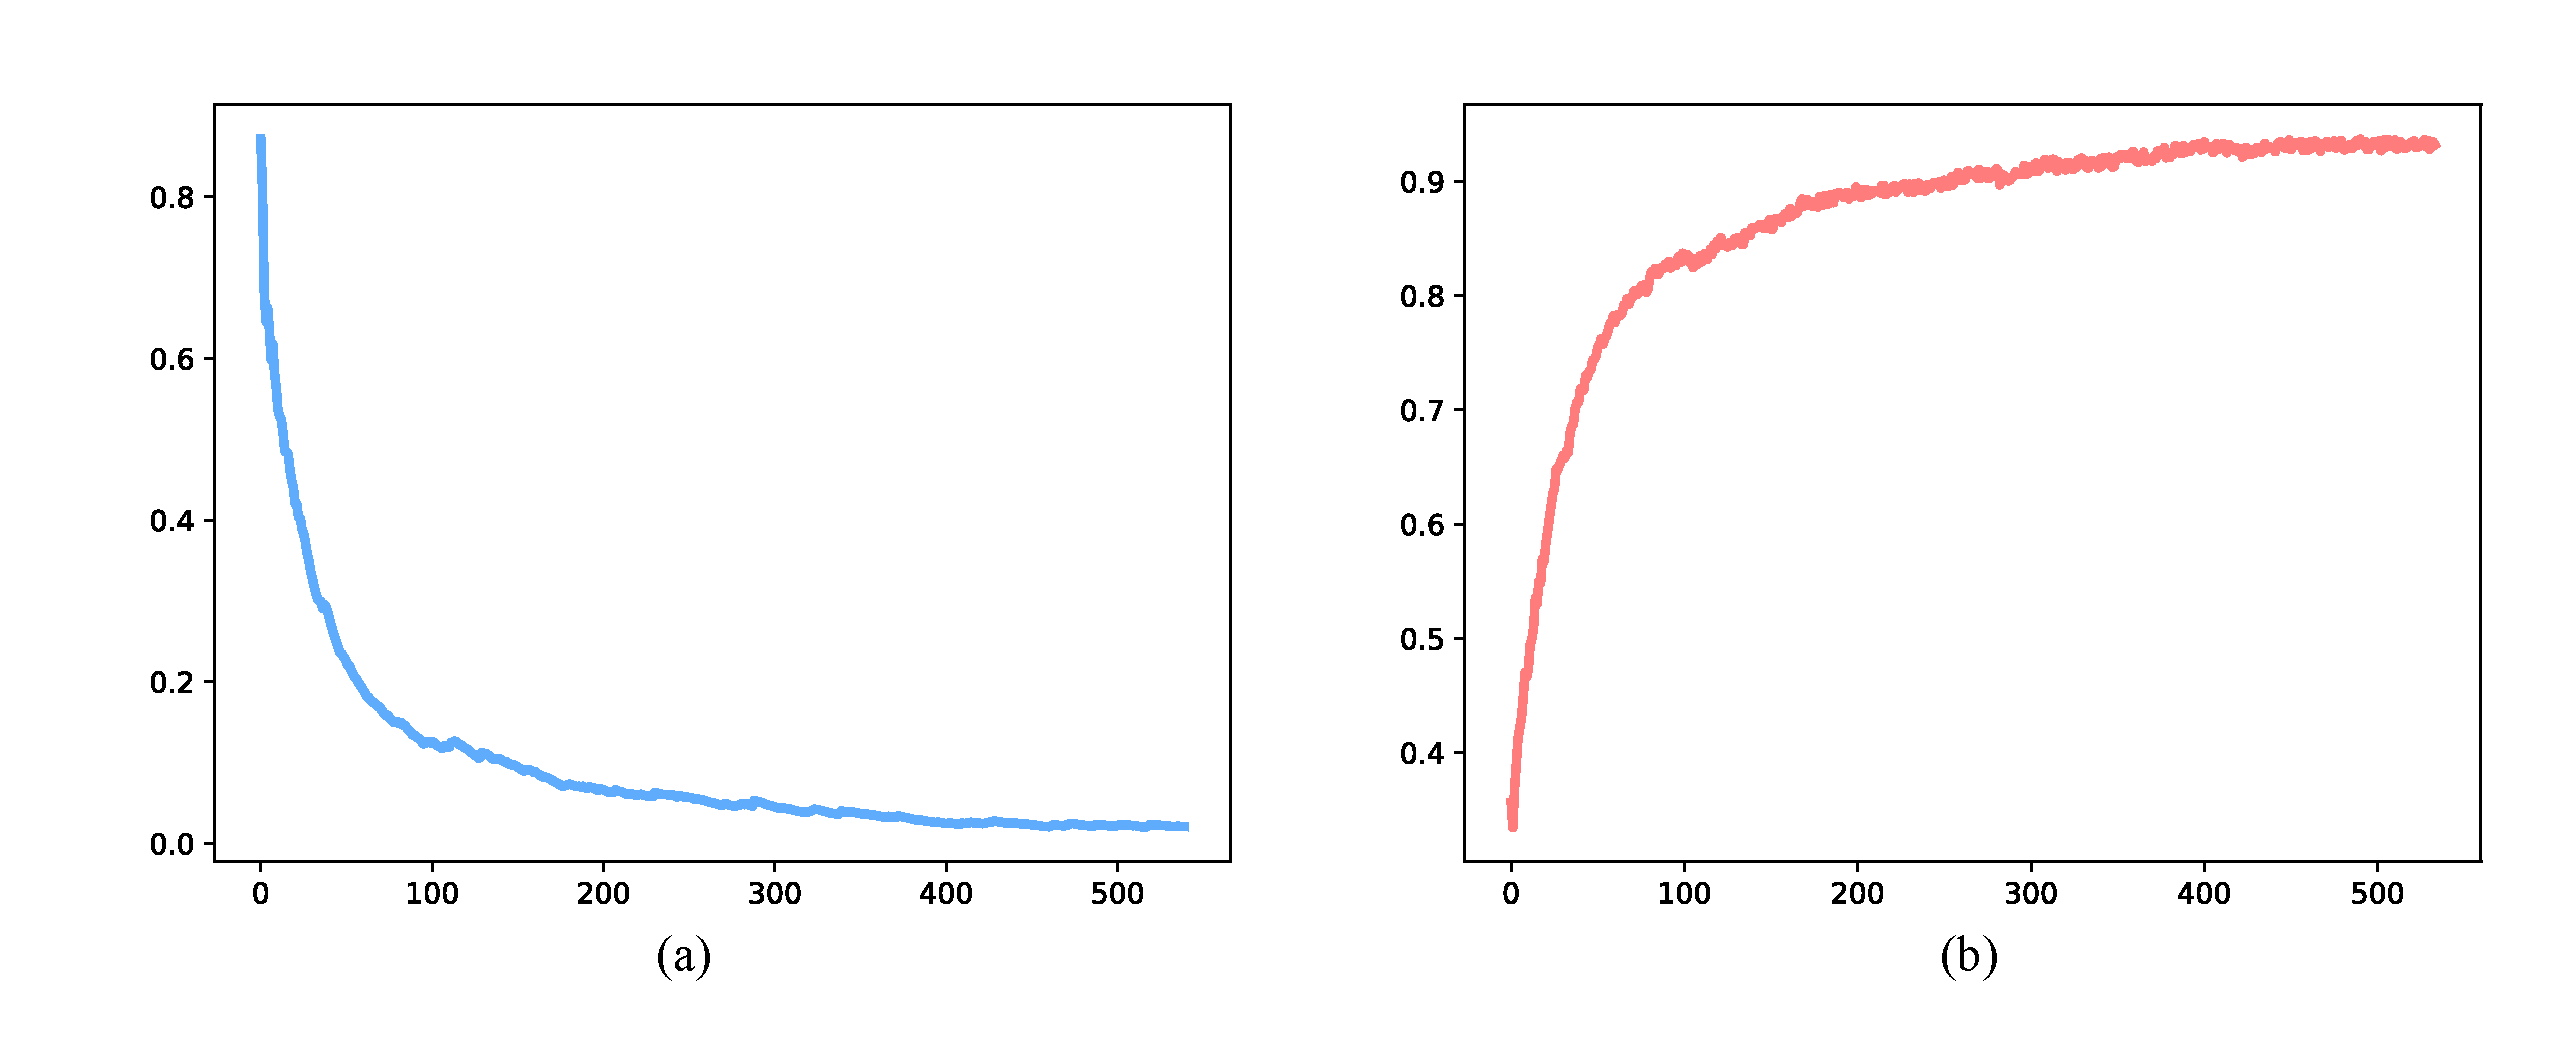
\includegraphics[width=15cm]{res_acc.pdf}
\caption{(a): Loss and (b): accuracy curve of \textsf{ResNet} during the training process.}
\label{resacc}
\end{figure}

}

\large{You are able to see the source code of this architecture in \textbf{Appendix. C.}}
%%%%%
\vspace{2mm}
\begin{center}
\large\textbf{Results} \\
\end{center}

\large{

\textbf{Fig. \ref{resresults}} shows the scatter plot of predicted values for 4000 samples and the histogram of predicted values for them. We find that most scatters lie in the scale of 0.0-0.2, meaning that columnar cactus are absent in most images taken by UAVs in the testing set. Plus, most answers are explicit (\textit{i.$\ $e.}, the results are relatively sured), for almost all scatters are distributed in 0-0.2 and 0.8-1 (\textit{i.$\ $e.}, high confidence intervals).

}

\begin{figure}[h]
\centering
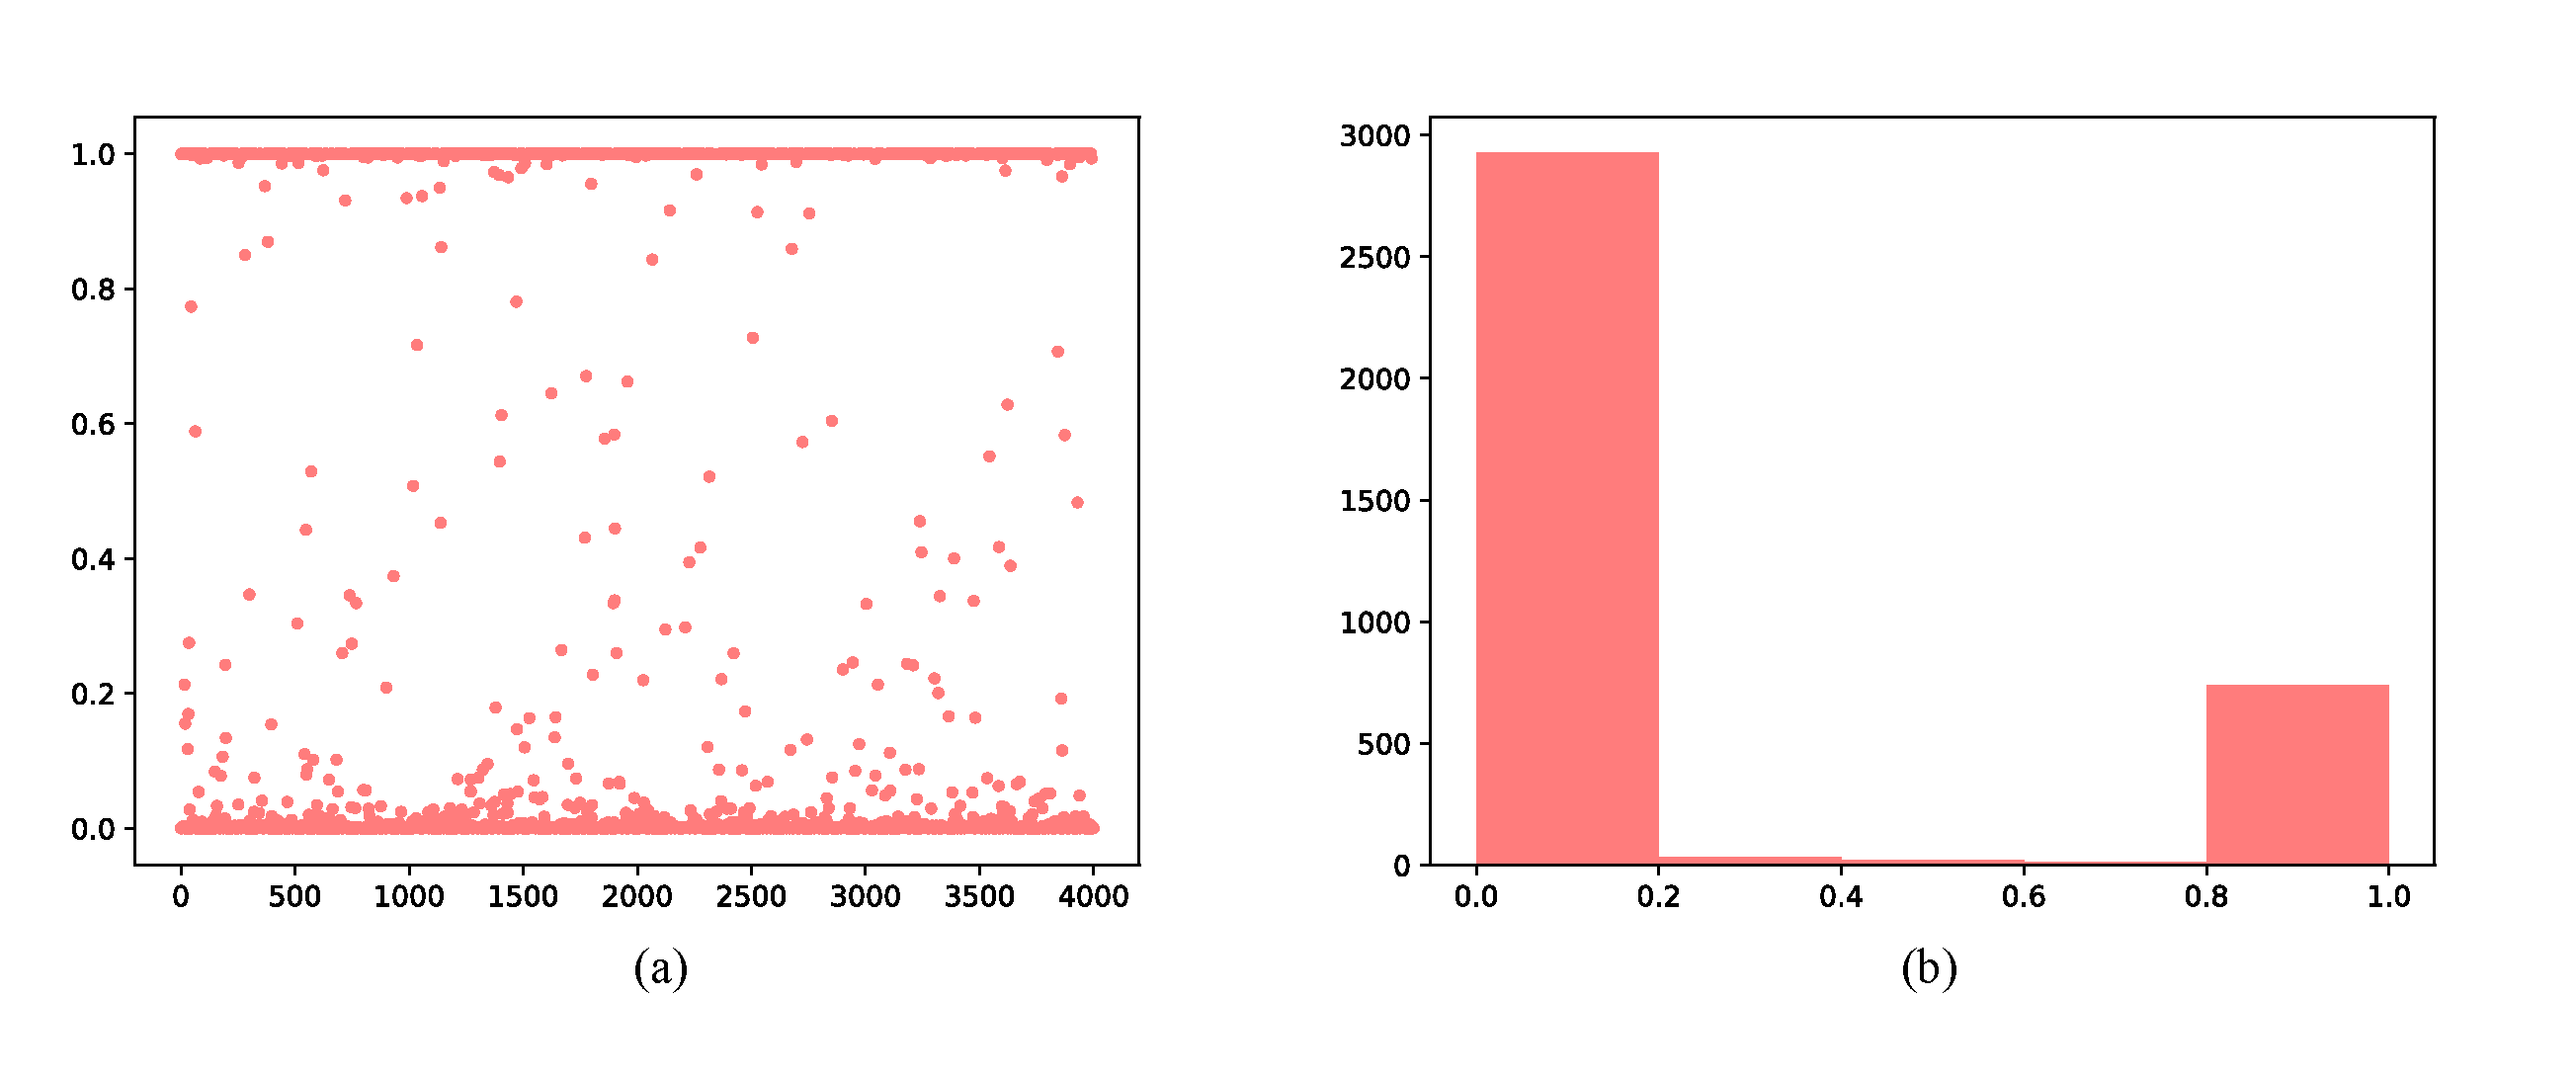
\includegraphics[width=15cm,height=6cm]{res_best.pdf}
\caption{ (a): Prediction scatter and (b): prediction histogram of \textsf{ResNet}.}
\label{resresults}
\end{figure}

%%%%%
\vspace{2mm}
\begin{center}
\large\textbf{Evaluation} \\
\end{center}
%resnet_101_1e-2_sgd_use-one-cycle_dofilp-flipvert
\large{
Our \textsf{ResNet} architecture has a up to \textbf{97.19\%} accuracy on the testing set when adopting the appropriate setting, (\textit{i.e.} 101 layer, 1e-2 learning rate, Adam optimizer, use one-cycle, and do nothing pre-processing). We also compare the impacts of parameters on the final score between different models as shown in \textbf{Fig. \ref{rescompare}}. We find that pre-processing techniques like flipping images have no huge impacts on the models' accuracies. Among the three models, \textsf{ResNet-101} perform the best and it's a rational measurement to exploit Adam optimizer in the models. Meanwhile, learning rate of 1e-2 is appropriate for training. The last sub-figure shows that one-cycle scheduler doesn't have huge effect on the overall performance. Note that all of the comparison is base on this baseline -- adopting flip techniques on \textsf{VGGNet-101} with a learning rate of 1e-2, using SGD optimizer and one-cycle scheduler.

\begin{figure}[h]
\centering
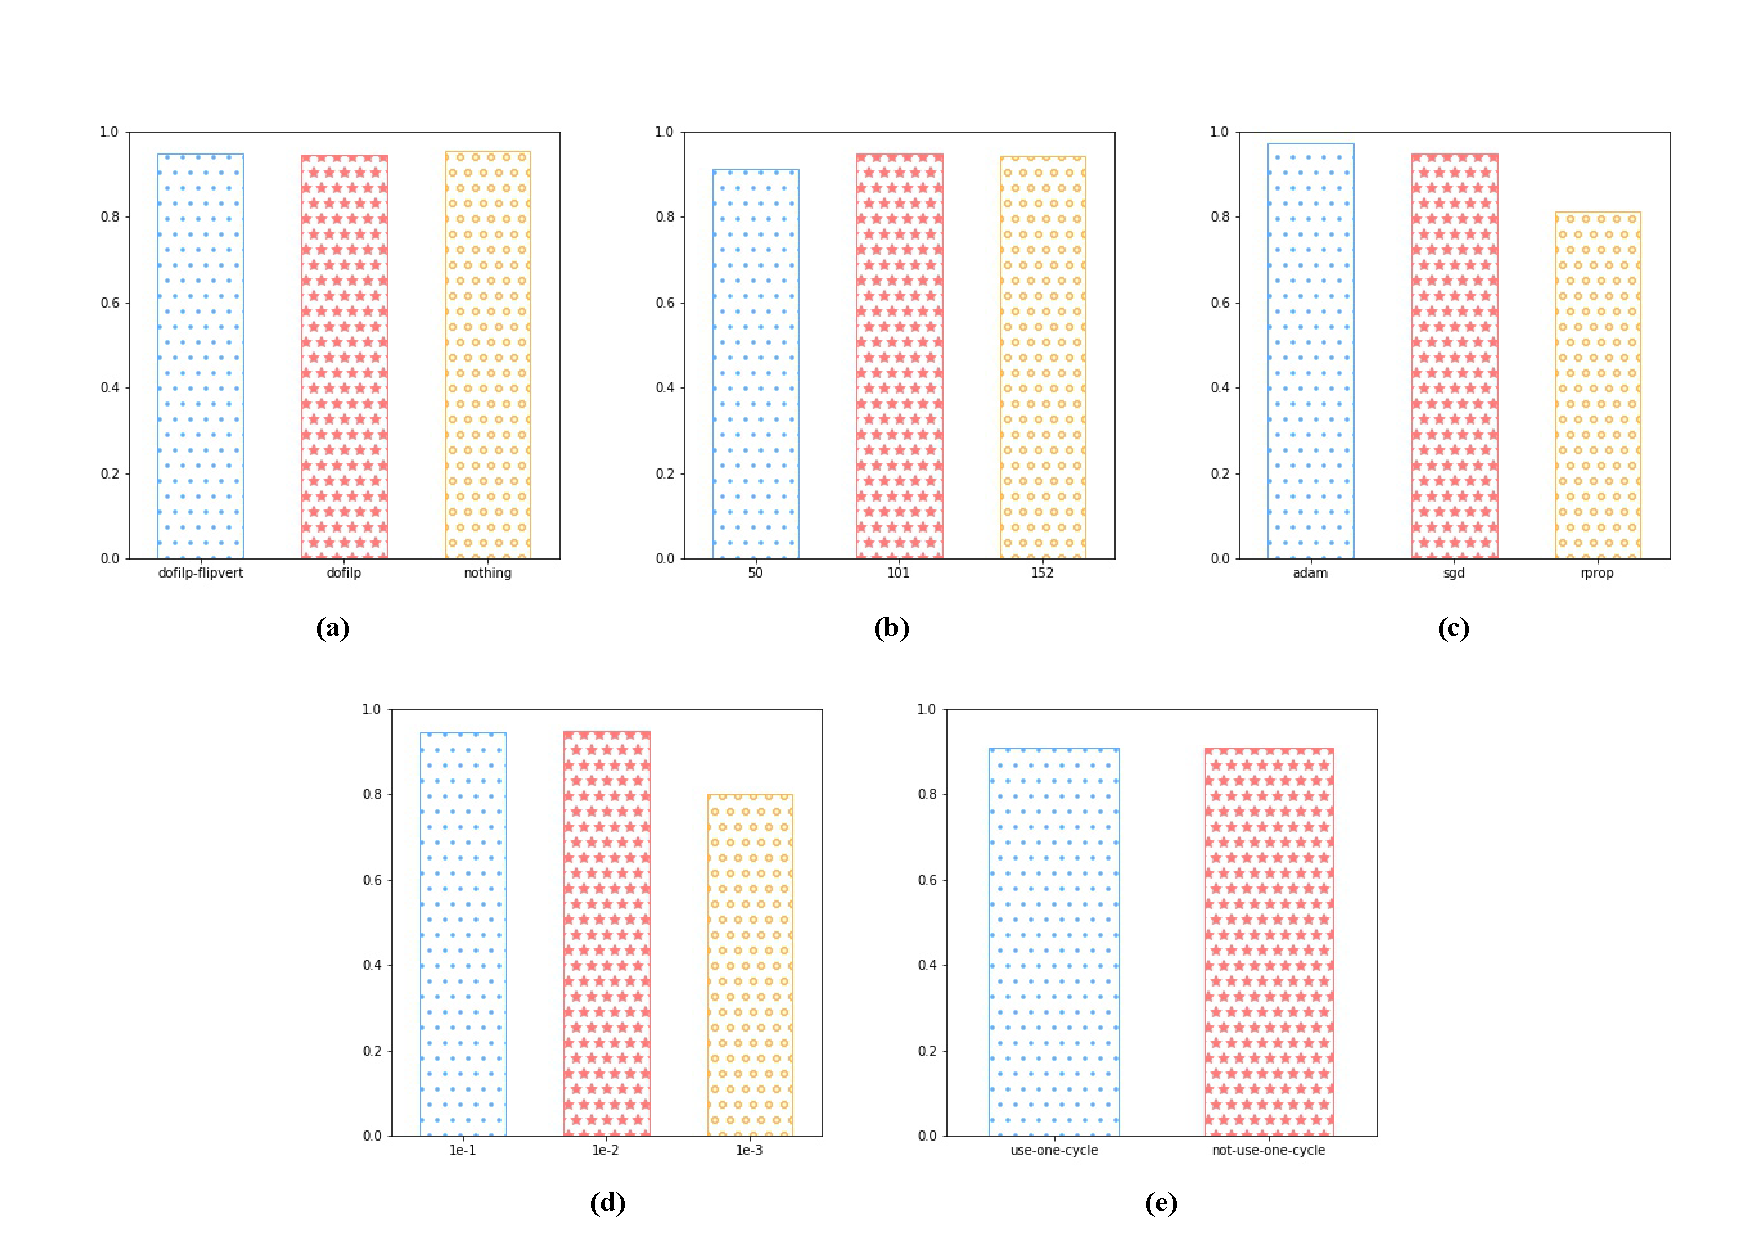
\includegraphics[width=15cm]{res.pdf}
\caption{ Impacts of (a): pre-processing techniques, (b): the number of layer, (c): optimizer, (d) learning rate, and (e) scheduler between different models of \textsf{ResNet}.}
\label{rescompare}
\end{figure}

}
\clearpage
%%% section V. Squeeze-and-Excitation -Res Neural Network
\vspace{5mm}
\begin{center}
\LARGE\textbf{V. ``Squeeze and Excitation'' Residual Network} \\
\end{center}
\vspace{2mm}

\large{You are able to see our kernel submission page in \textbf{Appendix. B.}}

\vspace{2mm}
\begin{center}
\large\textbf{Architecture} \\
\end{center}


\large{
We locate to \textsf{SEResNet} as our third architecture, for \textsf{SEResNet} is one of the enhancements of \textsf{ResNet}. Here, we build \textsf{SEResNet-50}, \textsf{SEResNet-101}, and \textsf{SEResNet-152} models in this framework.

\begin{figure}[h]
\centering
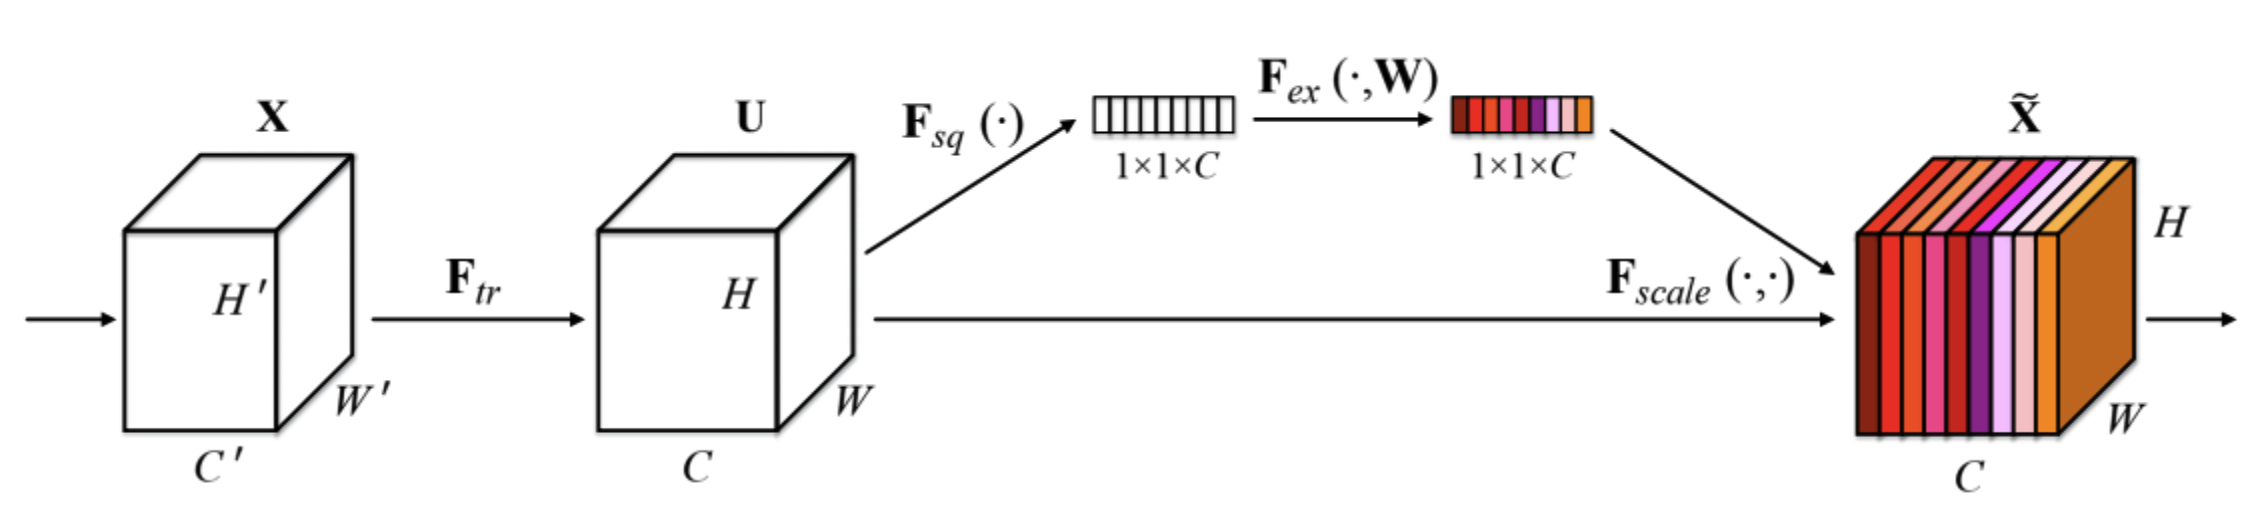
\includegraphics[width=15cm]{senet.png}
\caption{\textsf{SEResNet}: ``Squeeze and Excitation'' Residual Network architecture.}
\label{searc}
\end{figure}

Squeeze-and-Excitation Network (\textsf{SENet}) introduces a building block for CNN that improves channel interdependencies at almost no computational cost. The main idea of \textsf{SENet} is that ``\textit{let’s add parameters to each channel of a convolutional block so that the network can adaptively adjust the weighting of each feature map}''.

\begin{figure}[h]
\centering
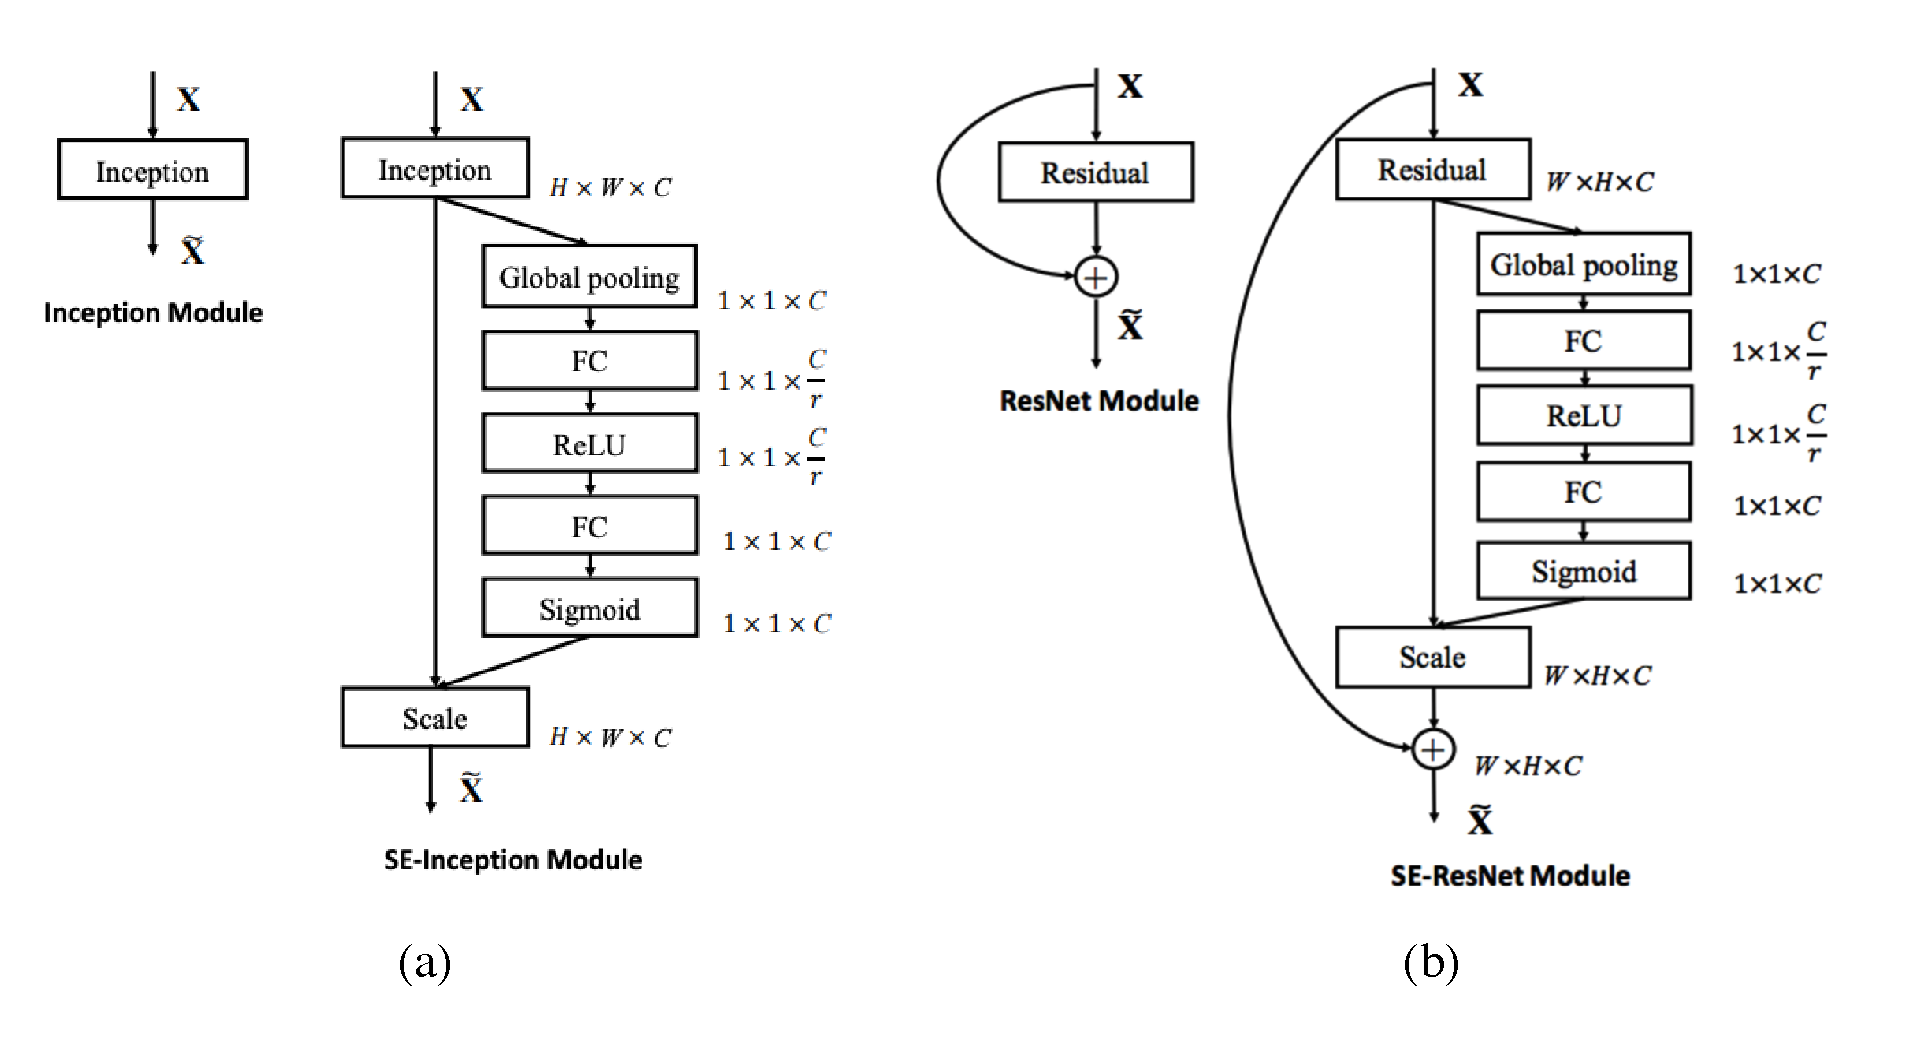
\includegraphics[width=15cm]{seblock.pdf}
\caption{\textsf{SEResNet}: ``Squeeze and Excitation'' Residual Network architecture.}
\label{seblock}
\end{figure}

When simply taking the transformation to be an entire Inception module (see \textbf{Fig. \ref{seblock} (a)}) and making this change for each such module in the architecture, we can get an SE-Inception network. SE blocks can also be used directly with residual networks (\textbf{Fig. \ref{seblock} (b)} depicts the schema of an \textsf{SEResNet} module). The SE block transformation is taken to be the non-identity branch of a residual module. ``Squeeze'' and ``Excitation'' both act before summation with the identity branch.

}

%%%%%
\vspace{2mm}
\begin{center}
\large\textbf{Implementation} \\
\end{center}

\large{

To implement \textsf{SEResNet},we construct  \textsf{SEResNet}-Bottleneck blocks based on bottleneck block of \textsf{ResNet}. For each \textsf{SEResNet} Bottleneck block, a SEModule and a down sample module are added to adaptively adjust weights of each feature map in the block. Each SEModule consists of one AdaptiveAvgPool2d layer and two Linear layers, and uses relu and sigmoid as activation function. Each down sample module consists of one Conv2d layer to down sample feature maps in the block.

The head of model uses two AdaptiveAvgPool2d layers to transform the output feature map of body to size [4096, 1, 1], and two linear layers (with out\_features = 512 and 2) to output score for each class. Batch normalization and dropout are used in head of model to avoid overfitting.

Each model is pre-trained. In addition, fine tunning method is used when training, with only parameters of BatchNorm layers and Linear layers trainable. For example, our \textsf{SEResNet-101} has 49385778 parameters in total. However, by fine tunning, only 2213250 parameters need to be trained.

The loss and accurate curve on the given training set is shown in \textbf{Fig. \ref{seres_acc}}. Note that the loss is decreased and the accuracy is improved with the training.

\begin{figure}[h]
\centering
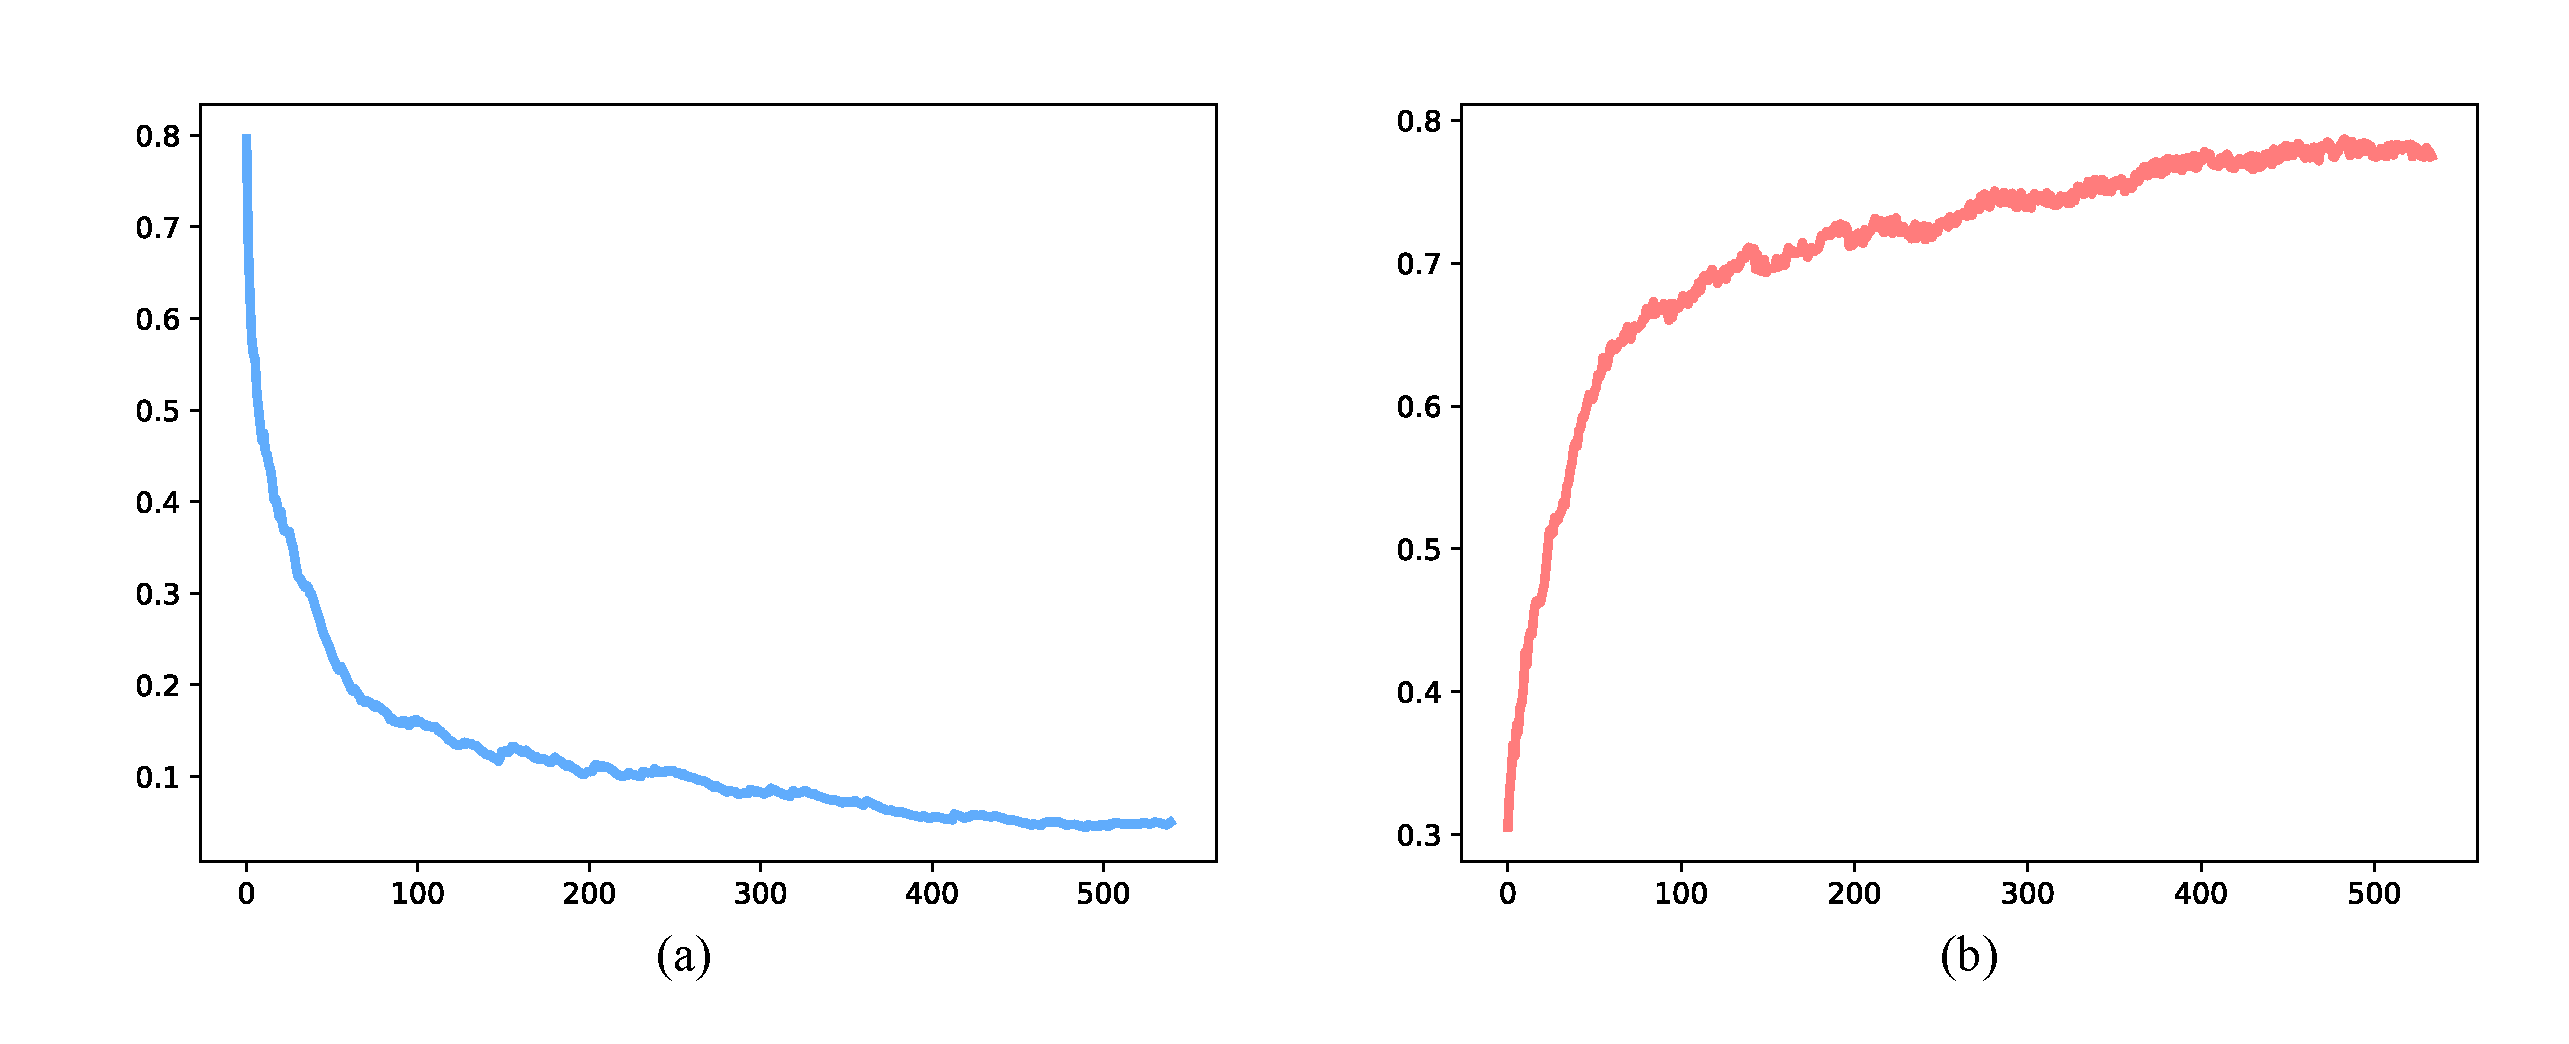
\includegraphics[width=15cm]{seres_acc.pdf}
\caption{(a): Loss and (b): accuracy curve of \textsf{SEResNet} during the training process.}
\label{seres_acc}
\end{figure}

}

\large{You are able to see the source code of this architecture in \textbf{Appendix. C.}}
%%%%%
\vspace{2mm}
\begin{center}
\large\textbf{Results} \\
\end{center}

\large{

\textbf{Fig. \ref{seresresults}} shows the scatter plot of predicted values for 4000 samples and the histogram of predicted values for them. We find that most scatters lie in the scale of 0.0-0.2, meaning that columnar cactus are absent in most images taken by UAVs in the testing set. Plus, most answers are explicit (\textit{i.$\ $e.}, the results are relatively sured), for almost all scatters are distributed in 0-0.2 and 0.8-1 (\textit{i.$\ $e.}, high confidence intervals).

}

\begin{figure}[h]
\centering
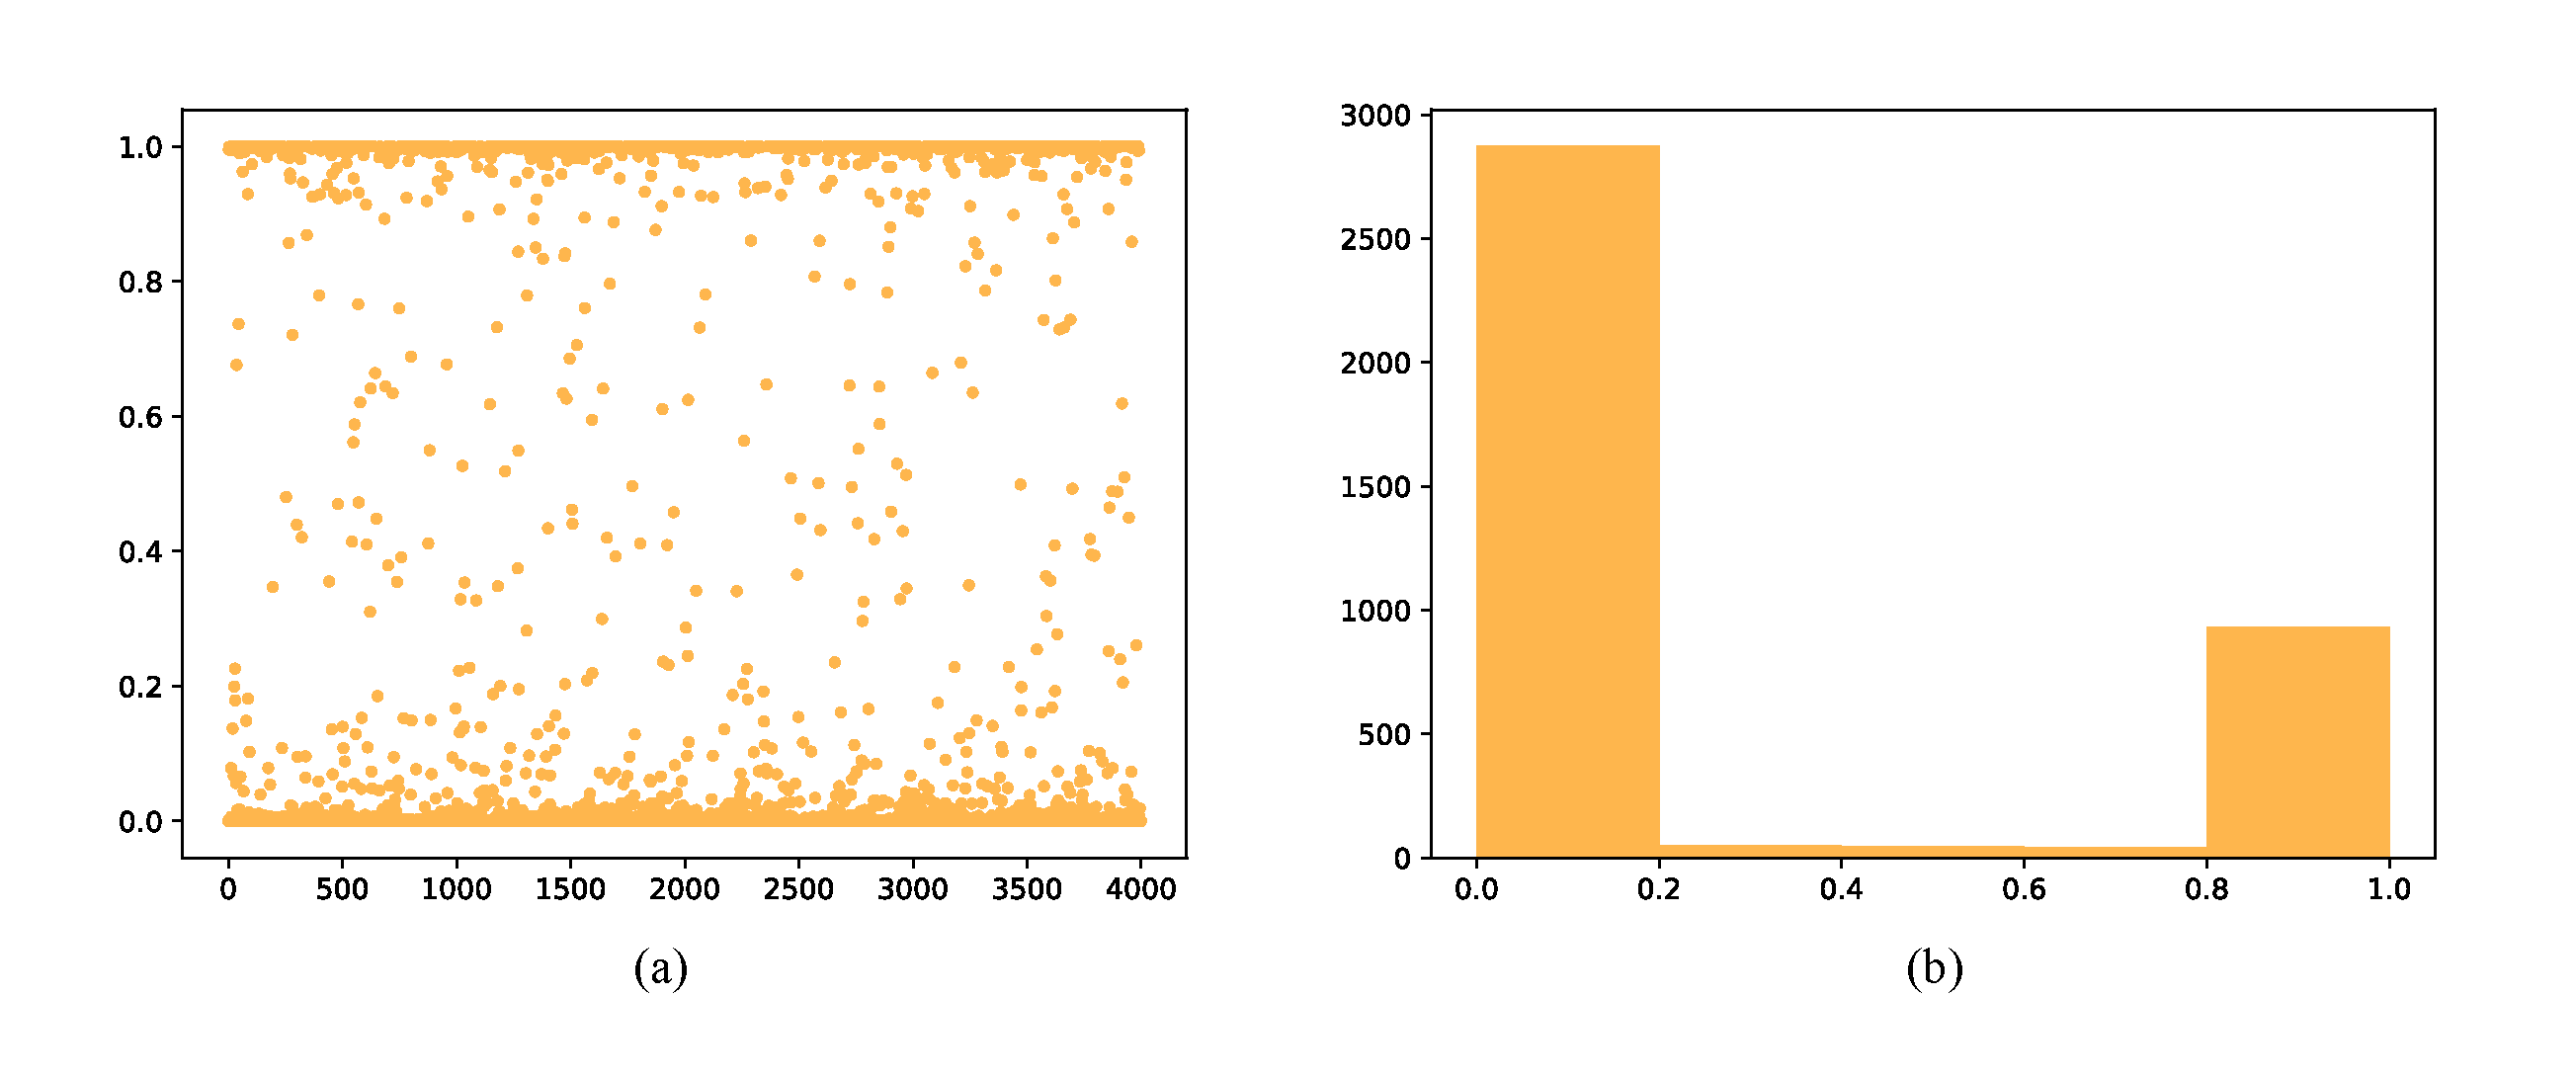
\includegraphics[width=15cm,height=6cm]{seres_best.pdf}
\caption{ (a): Prediction scatter and (b): prediction histogram of \textsf{SEResNet}.}
\label{seresresults}
\end{figure}

%%%%%
\vspace{2mm}
\begin{center}
\large\textbf{Evaluation} \\
\end{center}

%se_resnet_101_1e-2_sgd_use-one-cycle_dofilp-flipvert
\large{
Our \textsf{SEResNet} architecture has a up to \textbf{93.46\%} accuracy on the testing set when adopting the appropriate setting, (\textit{i.e.} 50 layer, 1e-1 learning rate, Adam optimizer, use one-cycle, and do no images pre-processing). We also compare the impacts of parameters on the final score between different models as shown in \textbf{Fig. \ref{serescompare}}. We find that pre-processing techniques like flipping images can not make the models more accurate, on the contrary, they even degrade the performance. Among the three models, \textsf{SEResNet-50} perform the best and it's a rational measurement to exploit Adam optimizer in the models. Meanwhile, learning rate of 1e-1 is appropriate for training. The last sub-figure shows that one-cycle scheduler doesn't have huge effect on the overall performance. Note that all of the comparison is base on this baseline -- adopting flip techniques on \textsf{SERNet-101} with a learning rate of 1e-2, using SGD optimizer and one-cycle scheduler.

\begin{figure}[h]
\centering
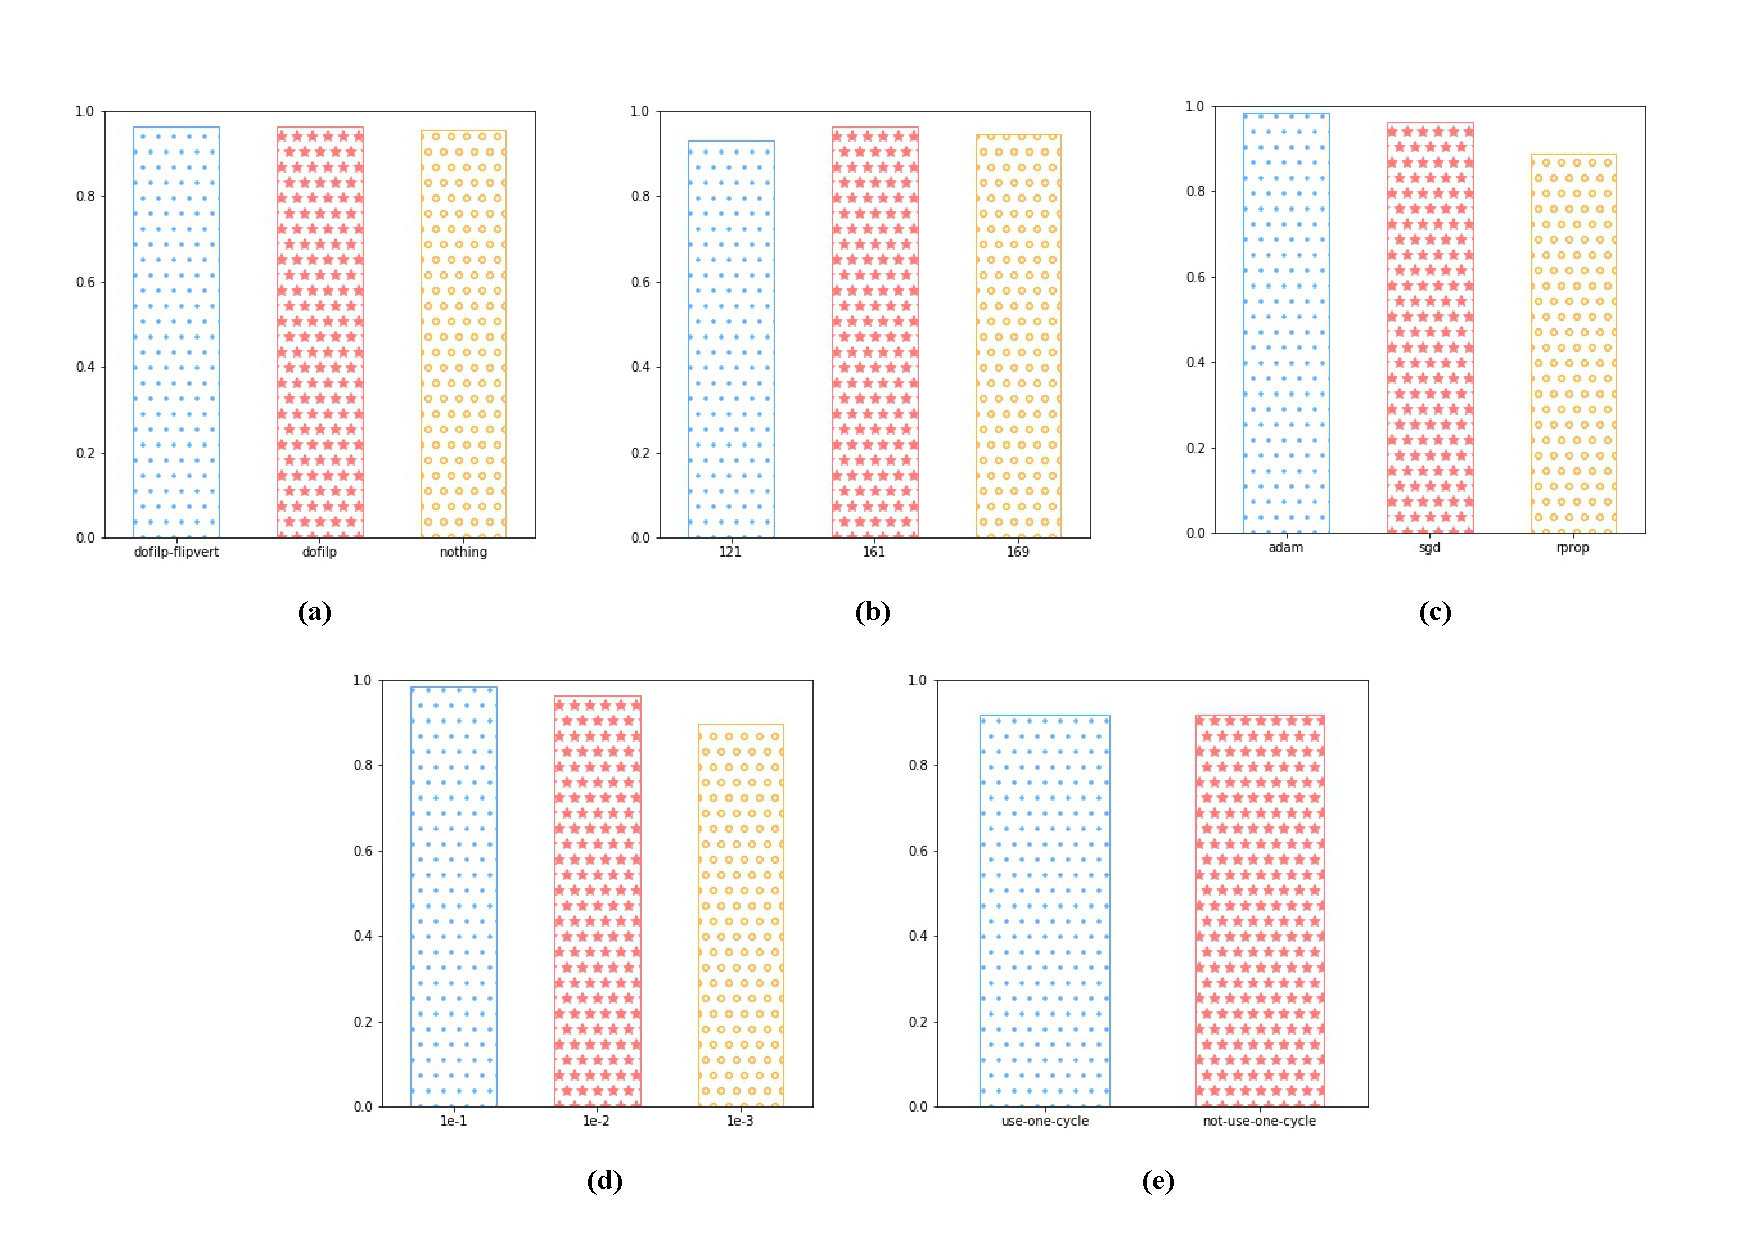
\includegraphics[width=15cm]{se-res.pdf}
\caption{ Impacts of (a): pre-processing techniques, (b): the number of layer, (c): optimizer, (d) learning rate, and (e) scheduler between different models of \textsf{SEResNet}.}
\label{serescompare}
\end{figure}

}

\clearpage
%%% section VI. Densely Connected Neural Network
\vspace{5mm}
\begin{center}
\LARGE\textbf{VI. Densely Connected Convolutional Network} \\
\end{center}
\vspace{2mm}

\large{You are able to see our kernel submission page in \textbf{Appendix. B.}}

\vspace{2mm}
\begin{center}
\large\textbf{Architecture} \\
\end{center}


\large{
In our forth architecture, after trials and errors, we locate to \textsf{DenseNet}. Here, we build \textsf{DenseNet-121}, \textsf{DenseNet-161}, and \textsf{DenseNet-169} models in this framework.

\begin{figure}[h]
\centering
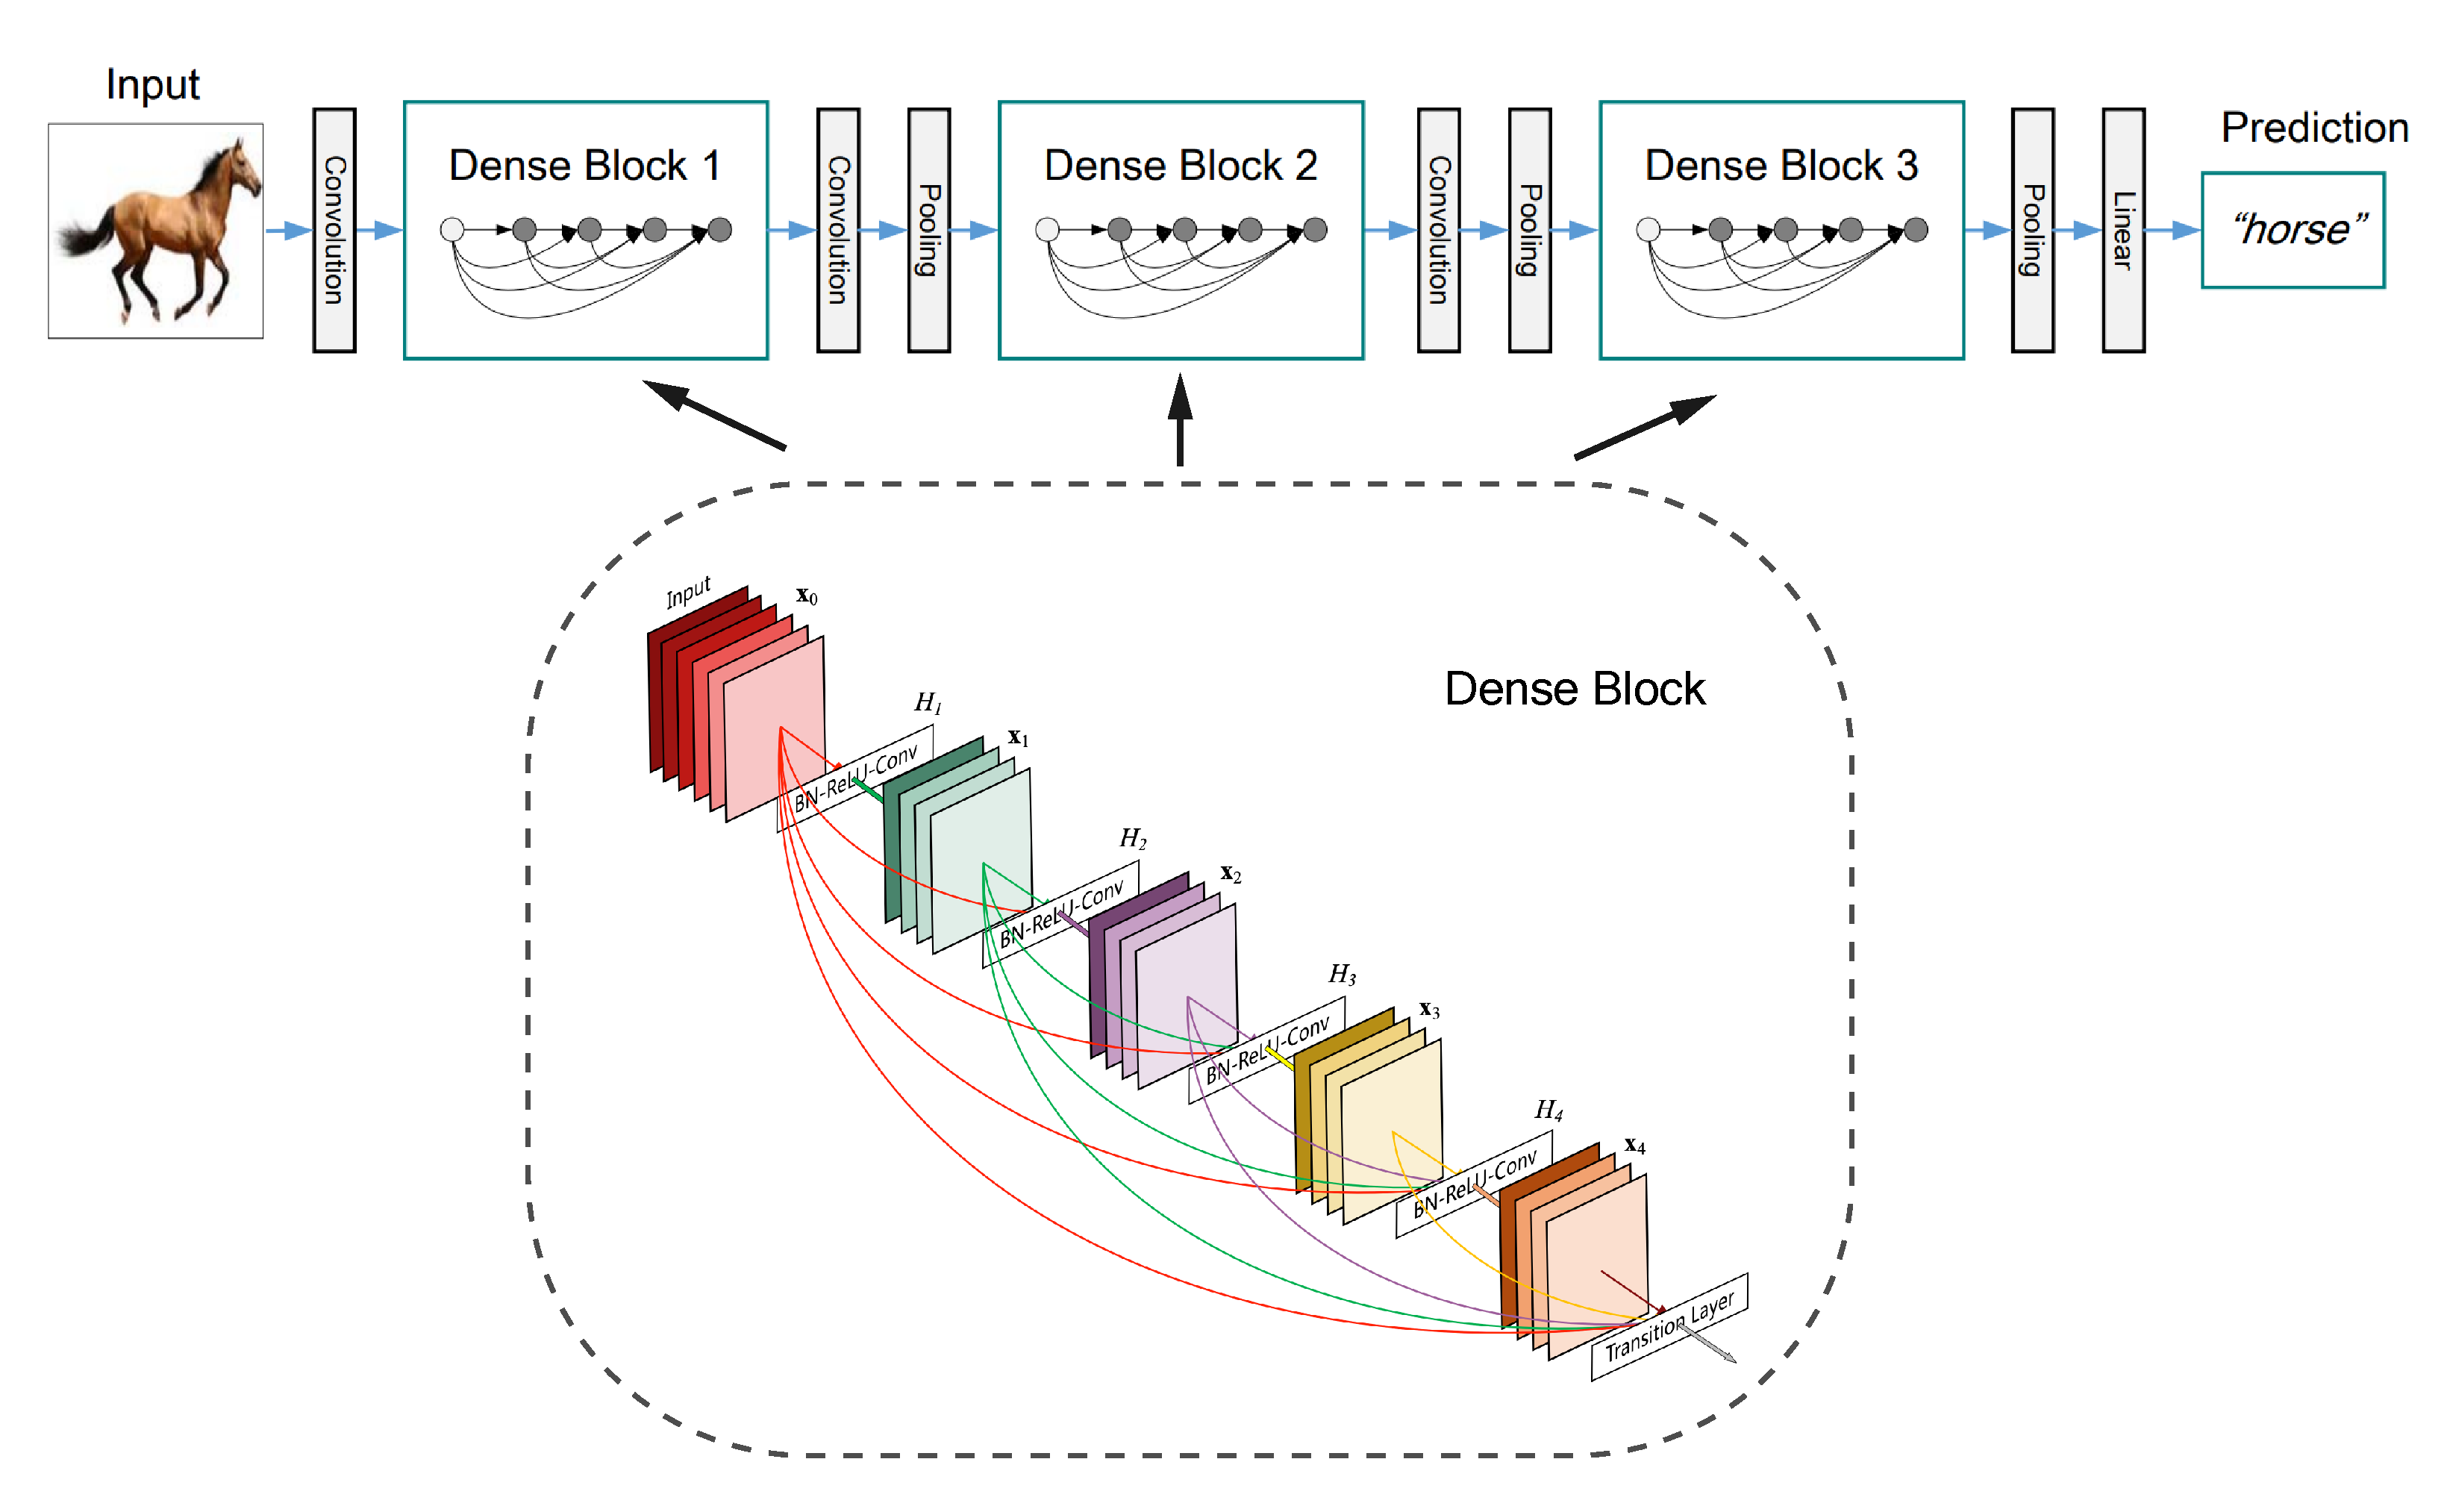
\includegraphics[width=15cm,height=9cm]{densenet.pdf}
\caption{\textsf{DenseNet}: Deeply Connected Convolutional Neural Network architecture.}
\label{densenetarch}
\end{figure}

Each layer of \textsf{DenseNet} is connected to the previous layer, enabling feature reuse. \textbf{Fig. \ref{densenetarch}} shows the framework of the dense block and its embedding in \textsf{DenseNet}. See that in a dense block, the input of layer $i$ is related not only to the output of layer $i-1$, but also to the output of all previous layers. In a dense block, the number of output channels by each nonlinear transform is constant. So the number of input channels at layer $i$ is $k+(i+1)* growth\_rate$, where $k$ is the number of input channels.

In dense block, the feature size does not change because the concatenate operation is required on the feature map of different layers, which needs to maintain the same feature size. Therefore, down-sampling is used in the adjacent dense block to increase the sensing field. In other words, the transition layer is used to realize it. Moreover, bottlenect structure are supposed to be used in \textsf{DenseNet} to reduce parameters and computations.

}

%%%%%
\vspace{2mm}
\begin{center}
\large\textbf{Implementation} \\
\end{center}

\large{

To implement \textsf{DenseNet},we construct DenseBlocks as basic blocks. Each DenseBlock consists of multiple DenseLayers which are connected densely. Each DenseLayer has a structure of "squential([norm1, relu1, conv1, norm2, relu2, conv2])". Based on DenseBlocks, we connect the blocks in similar way as \textsf{ResNet} to form the body of model.

The head of model uses two AdaptiveAvgPool2d layers to transform the output feature map of body to size [4096, 1, 1], and two linear layers (with out\_features = 512 and 2) to output score for each class. Batch normalization and dropout are used in head of model to avoid overfitting.

Each model is pre-trained. In addition, fine tunning method is used when training, with only parameters of BatchNorm layers and Linear layers trainable. For example, our \textsf{DenseNet-169} has 28744386 parameters in total. However, by fine tunning, only 2492322 parameters need to be trained.

The loss and accurate curve on the given training set is shown in \textbf{Fig. \ref{denseacc}}. Note that the loss is decreased and the accuracy is improved with the training.

\begin{figure}[h]
\centering
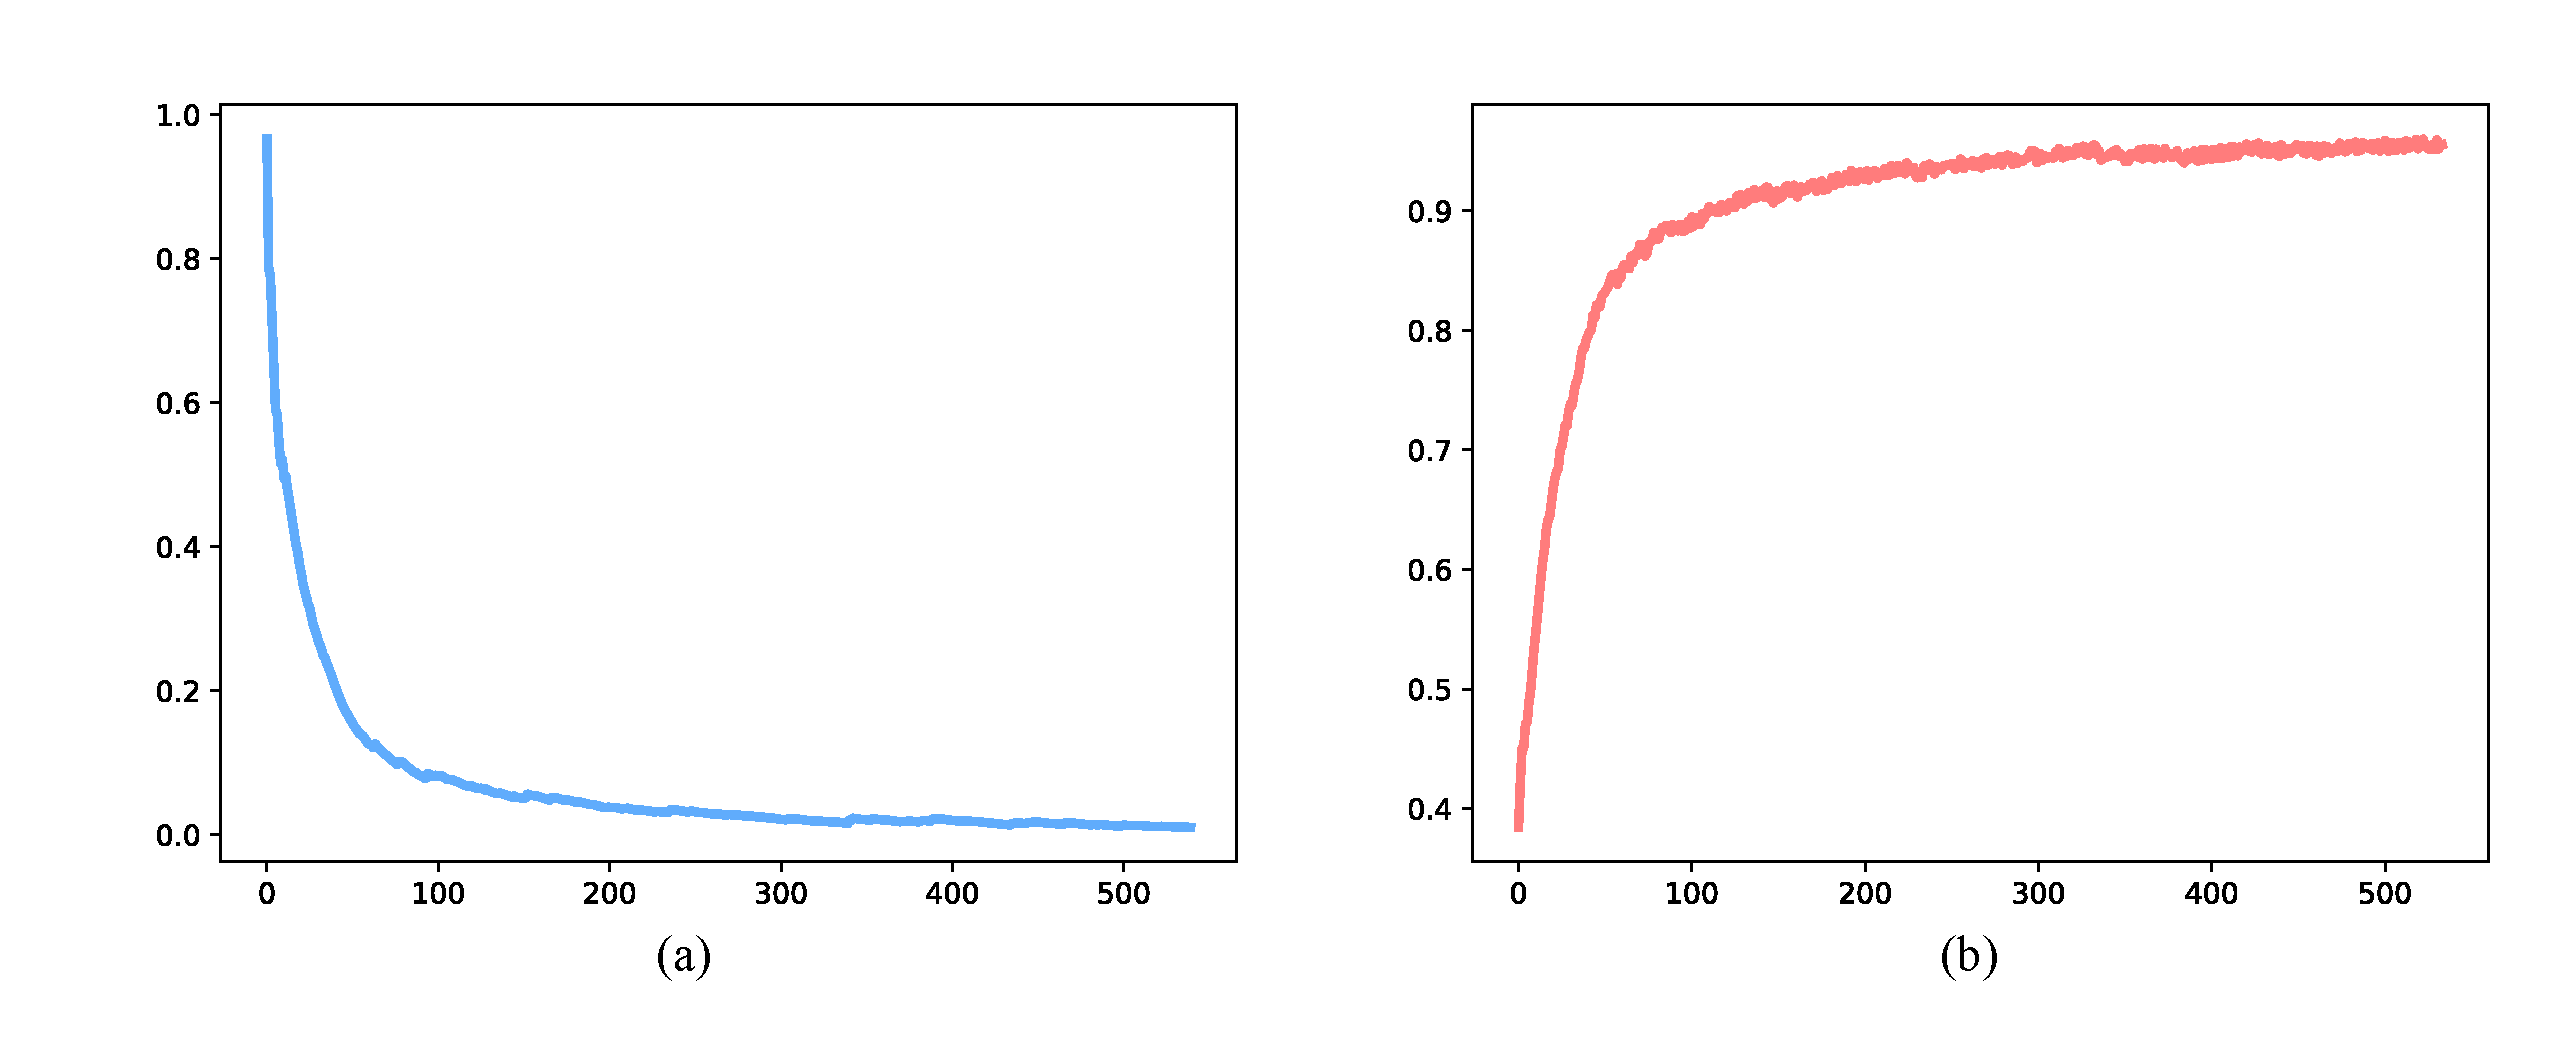
\includegraphics[width=15cm]{dense_acc.pdf}
\caption{(a): Loss and (b): accuracy curve of \textsf{DenseNet} during the training process.}
\label{denseacc}
\end{figure}

}

\large{You are able to see the source code of this architecture in \textbf{Appendix. C.}}
%%%%%
\vspace{2mm}
\begin{center}
\large\textbf{Results} \\
\end{center}

\large{

\textbf{Fig. \ref{denseresults}} shows the scatter plot of predicted values for 4000 samples and the histogram of predicted values for them. We find that most scatters lie in the scale of 0.0-0.2, meaning that columnar cactus are absent in most images taken by UAVs in the testing set. Plus, most answers are explicit (\textit{i.$\ $e.}, the results are relatively sured), for almost all scatters are distributed in 0-0.2 and 0.8-1 (\textit{i.$\ $e.}, high confidence intervals).

}

\begin{figure}[h]
\centering
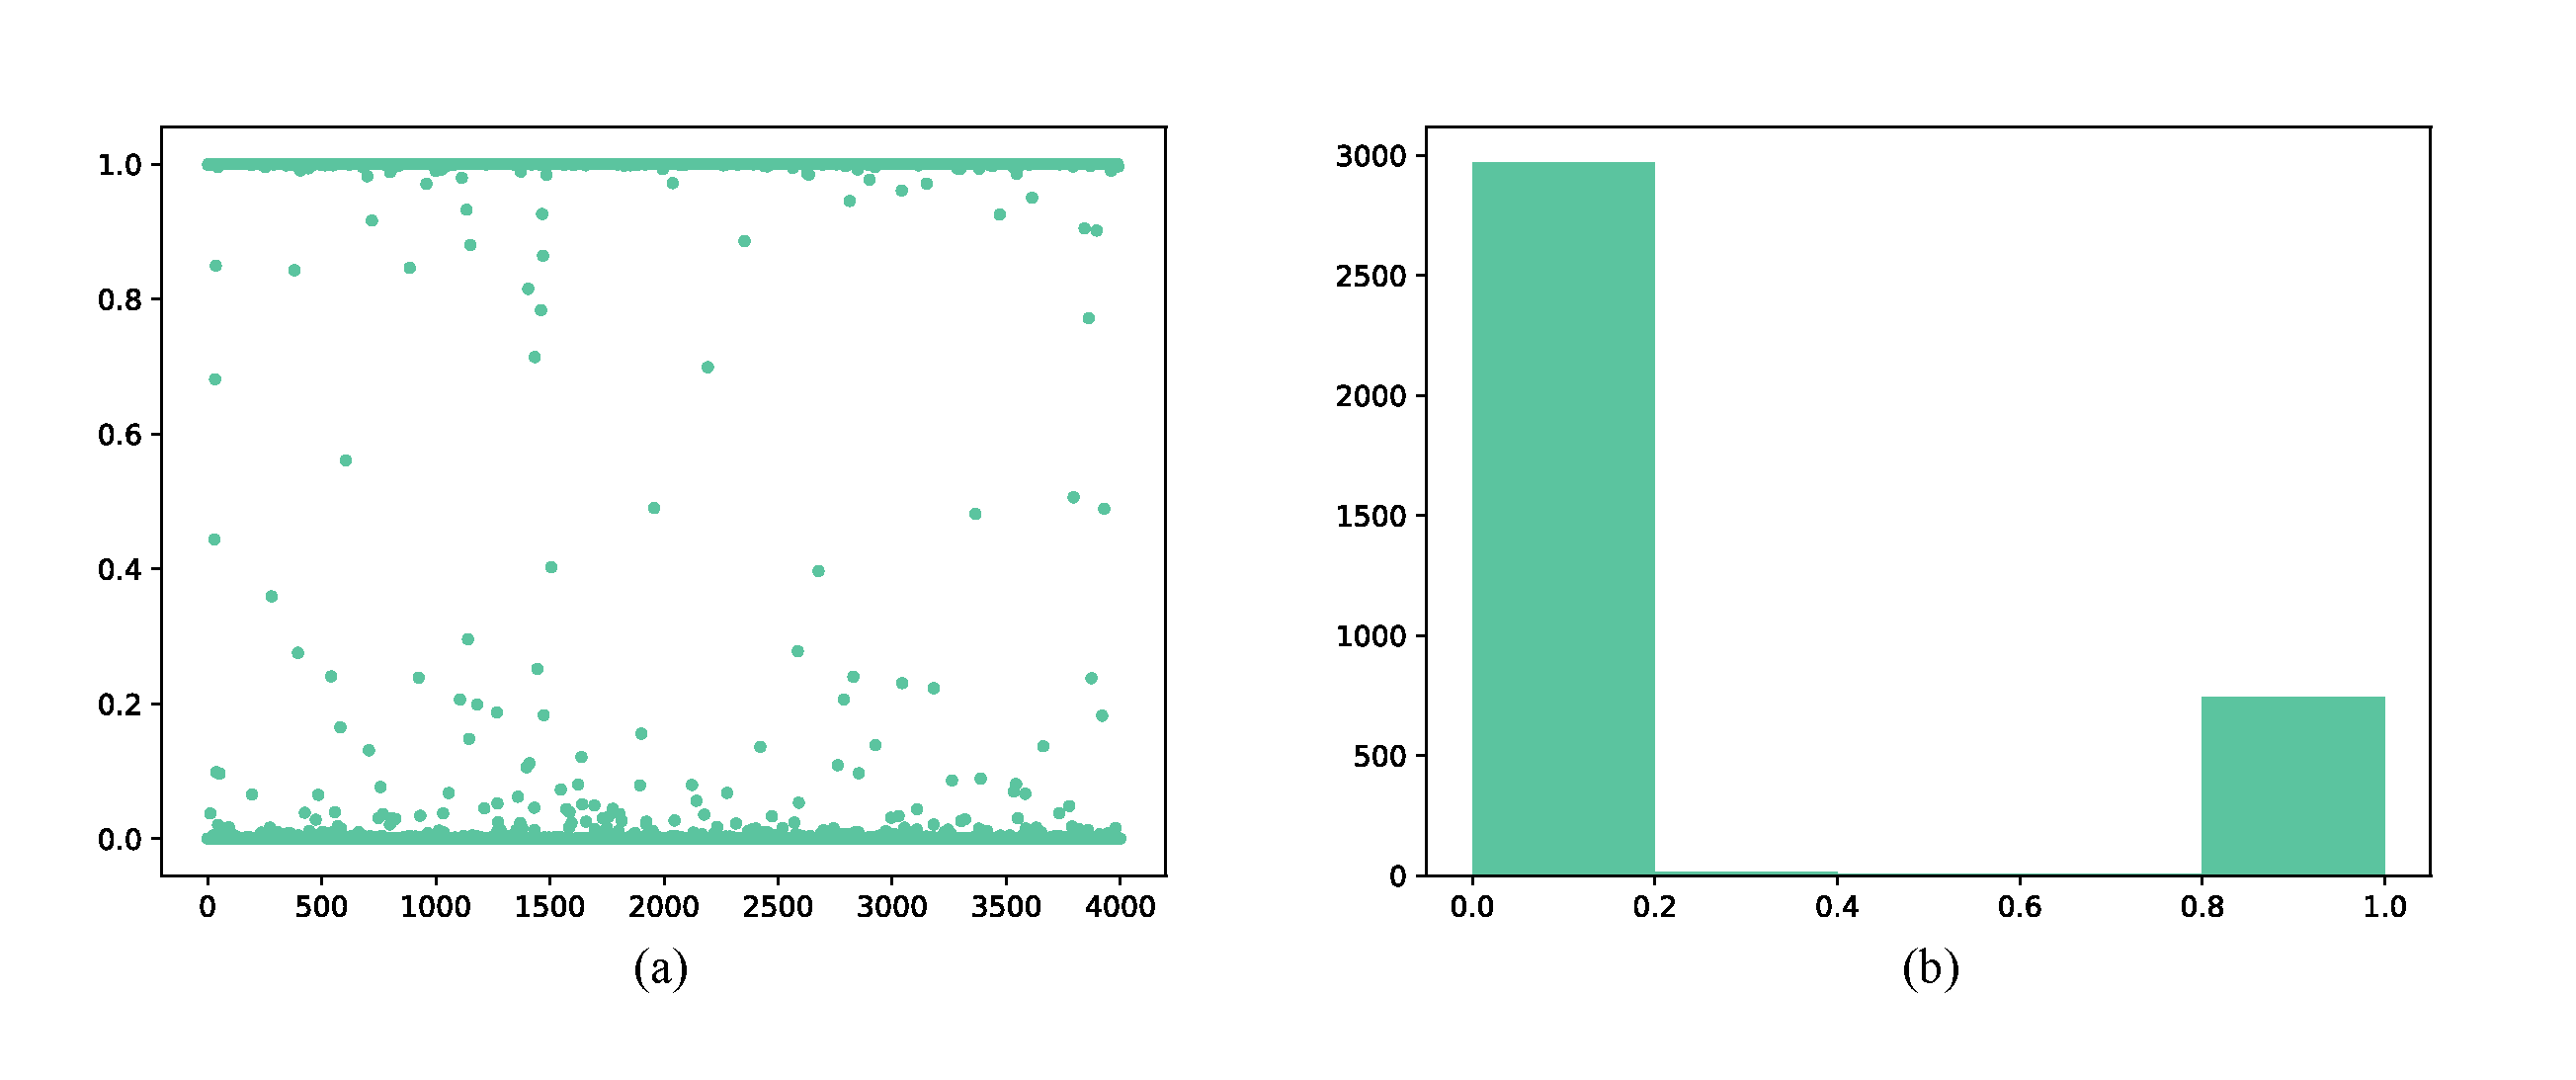
\includegraphics[width=15cm,height=6cm]{dense_best.pdf}
\caption{ (a): Prediction scatter and (b): prediction histogram of \textsf{DenseNet}.}
\label{denseresults}
\end{figure}

%%%%%
\vspace{2mm}
\begin{center}
\large\textbf{Evaluation} \\
\end{center}

%densenet_161_1e-2_sgd_use-one-cycle_dofilp-flipvert
\large{
Our \textsf{DenseNet} architecture has a up to \textbf{98.56\%} accuracy on the testing set when adopting the appropriate setting, (\textit{i.e.} 161 layer, 1e-1 learning rate, Adam optimizer, use one-cycle, and fliping the images). We also compare the impacts of parameters on the final score between different models as shown in \textbf{Fig. \ref{densecompare}}. We find that pre-processing techniques like flipping images can make the models more accurate. Among the three models, \textsf{DenseNet-161} perform the best and it's a rational measurement to exploit Adam optimizer in the models. Meanwhile, learning rate of 1e-1 is appropriate for training. The last sub-figure shows that one-cycle scheduler doesn't have huge effect on the overall performance. Note that all of the comparison is base on this baseline -- adopting flip techniques on \textsf{DenseNet-161} with a learning rate of 1e-2, using SGD optimizer and one-cycle scheduler.

\begin{figure}[h]
\centering
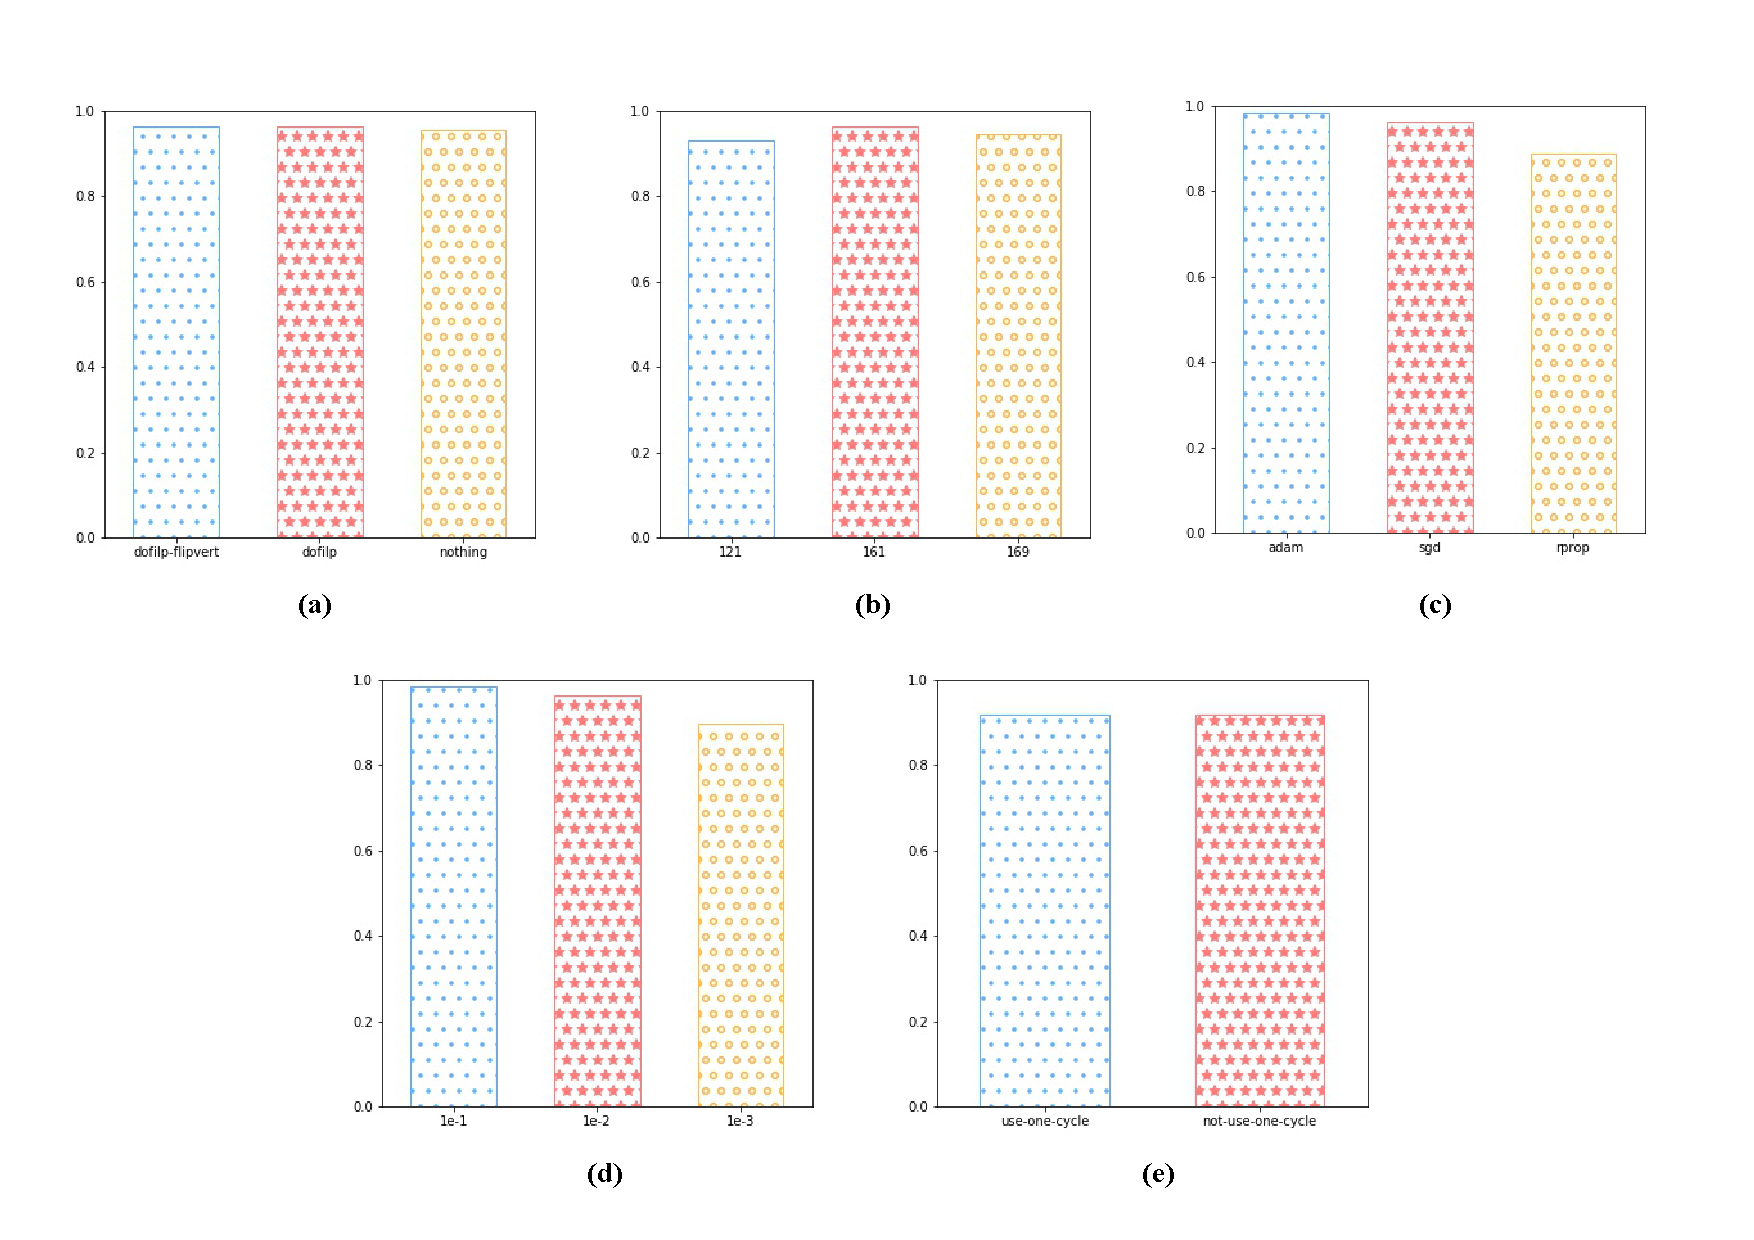
\includegraphics[width=15cm]{dense.pdf}
\caption{ Impacts of (a): pre-processing techniques, (b): the number of layer, (c): optimizer, (d) learning rate, and (e) scheduler between different models of \textsf{DenseNet}.}
\label{densecompare}
\end{figure}

}
\clearpage
%%% section VII. ResidualX Neural Network
\vspace{5mm}
\begin{center}
\LARGE\textbf{VII. Aggregated Residual Neural Networks} \\
\end{center}
\vspace{2mm}

\large{You are able to see our kernel submission page in \textbf{Appendix. B.}}

\vspace{2mm}
\begin{center}
\large\textbf{Architecture} \\
\end{center}


\large{
In our last architecture, after trials and errors, we locate to \textsf{ResNeXt}. Here, we build \textsf{ResNeXt-50} and \textsf{ResNeXt-101} models in this framework.

The \textsf{ResNeXt} was the first runner-up in the \texttt{2016 ILSVRC competition}. On top of the \textsf{ResNet}, \textsf{ResNeXt}'s next dimension is the cardinality dimension, where cardinality is the number of repeated layers.

\begin{figure}[h]
\centering
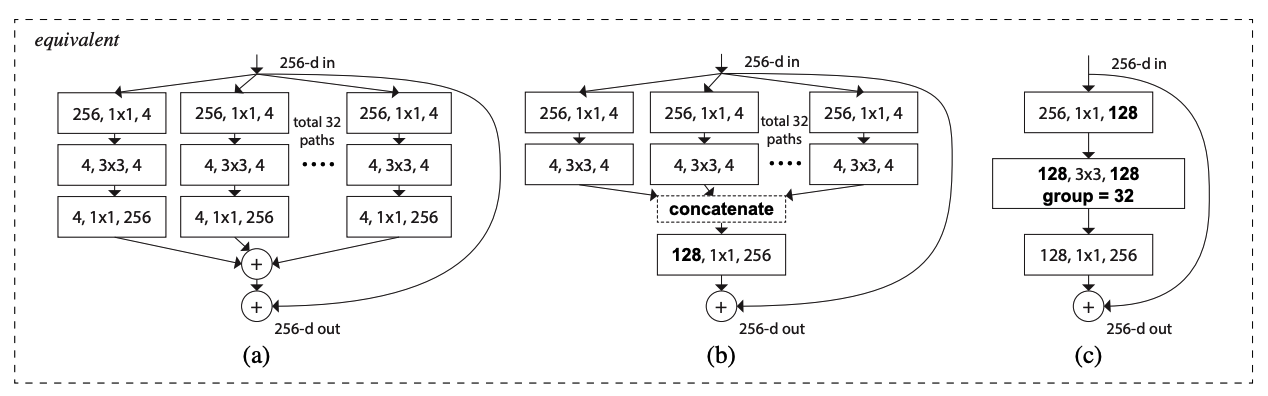
\includegraphics[width=15cm]{resnextblock.png}
\caption{Equivalent building blocks of \textsf{ResNeXt}.}
\label{resxblock}
\end{figure}

There are three equivalent \textsf{ResNeXt} blocks, as shown in \textbf{Fig. \ref{resxblock}}, (a) is the basic unit of \textsf{ResNeXt} (aggregated residual transformations). If the output is combined, equivalent network (b) has a similar structure to Inception-\textsf{ResNet} (early concatenation). And further if input is also combined, equivalent network (c) has a similar structure to the network of channel grouping convolution (grouped convolutions).

\begin{figure}[h]
\centering
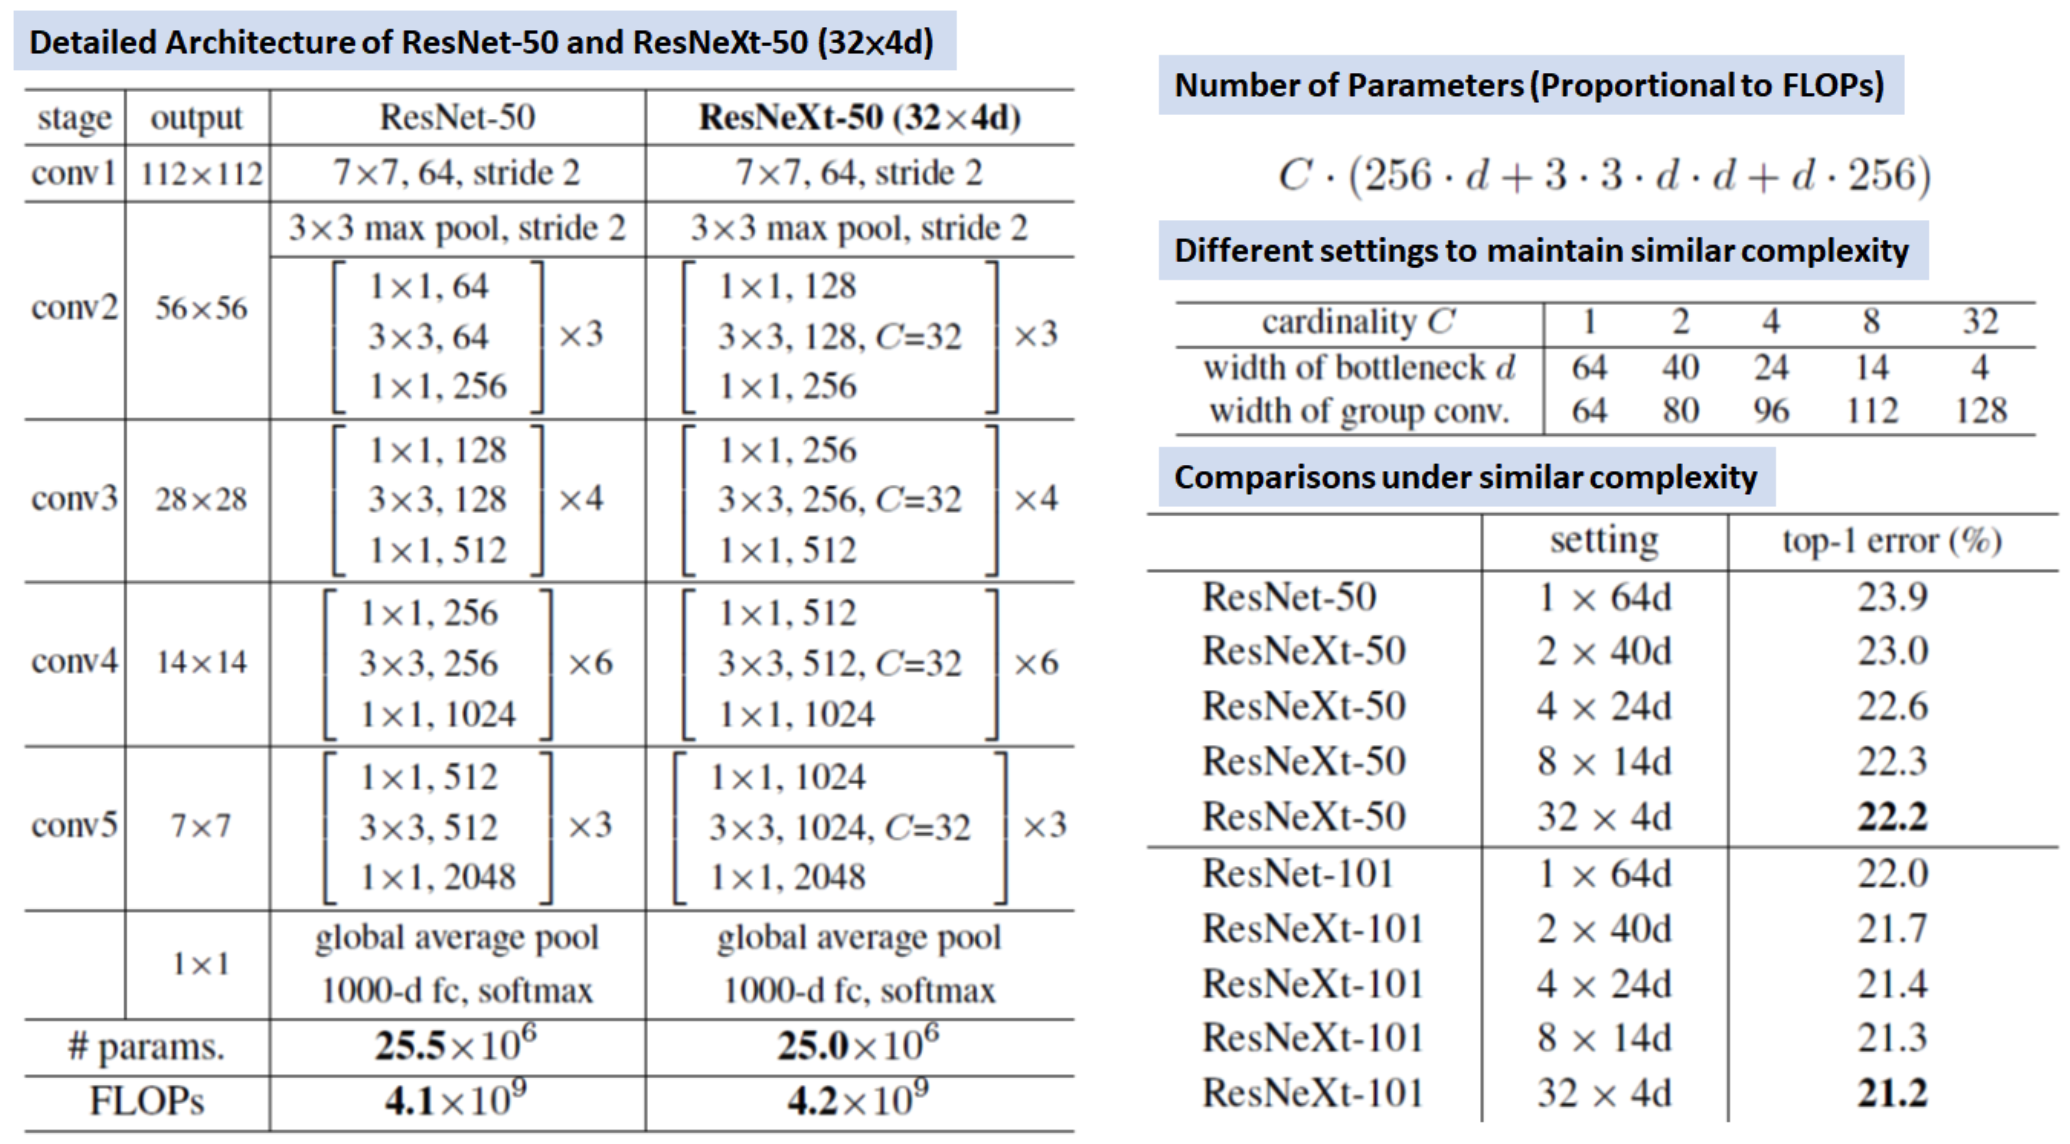
\includegraphics[width=15cm]{detailedarcresX.png}
\caption{Full Architecture and ablation study.}
\label{resxblockdetailedarc}
\end{figure}

\textbf{Fig. \ref{resxblockdetailedarc}} shows the detailed architecture of \textsf{ResNeXt} (left); number of parameters for each block (top right); different settings to maintain similar complexity (middle right), ablation study for different settings under similar complexity (bottom right).

}

%%%%%
\vspace{2mm}
\begin{center}
\large\textbf{Implementation} \\
\end{center}

\large{

To implement \textsf{ResNeXt},we also use Bottleneck of \textsf{ResNet} as basic block, and add one downs ample module to each block. However, convolution layers inside \textsf{ResNeXt} basic block are connected in way of aggregated residual transformations, namely group convolutions. And multiple \textsf{ResNeXt} basic blocks are connected to form the body of model.

The head of model uses two AdaptiveAvgPool2d layers to transform the output feature map of body to size [4096, 1, 1], and two linear layers (with out\_features = 512 and 2) to output score for each class. Batch normalization and dropout are used in head of model to avoid overfitting.

Each model is pre-trained. In addition, fine tunning method is used when training, with only parameters of BatchNorm layers and Linear layers trainable. For example, our \textsf{ResNeXt-101} has 88850242 parameters in total. However, by fine tunning, only 2310786 parameters need to be trained.

The loss and accurate curve on the given training set is shown in \textbf{Fig. \ref{resxacc}}. Note that the loss is decreased and the accuracy is improved with the training.

\begin{figure}[h]
\centering
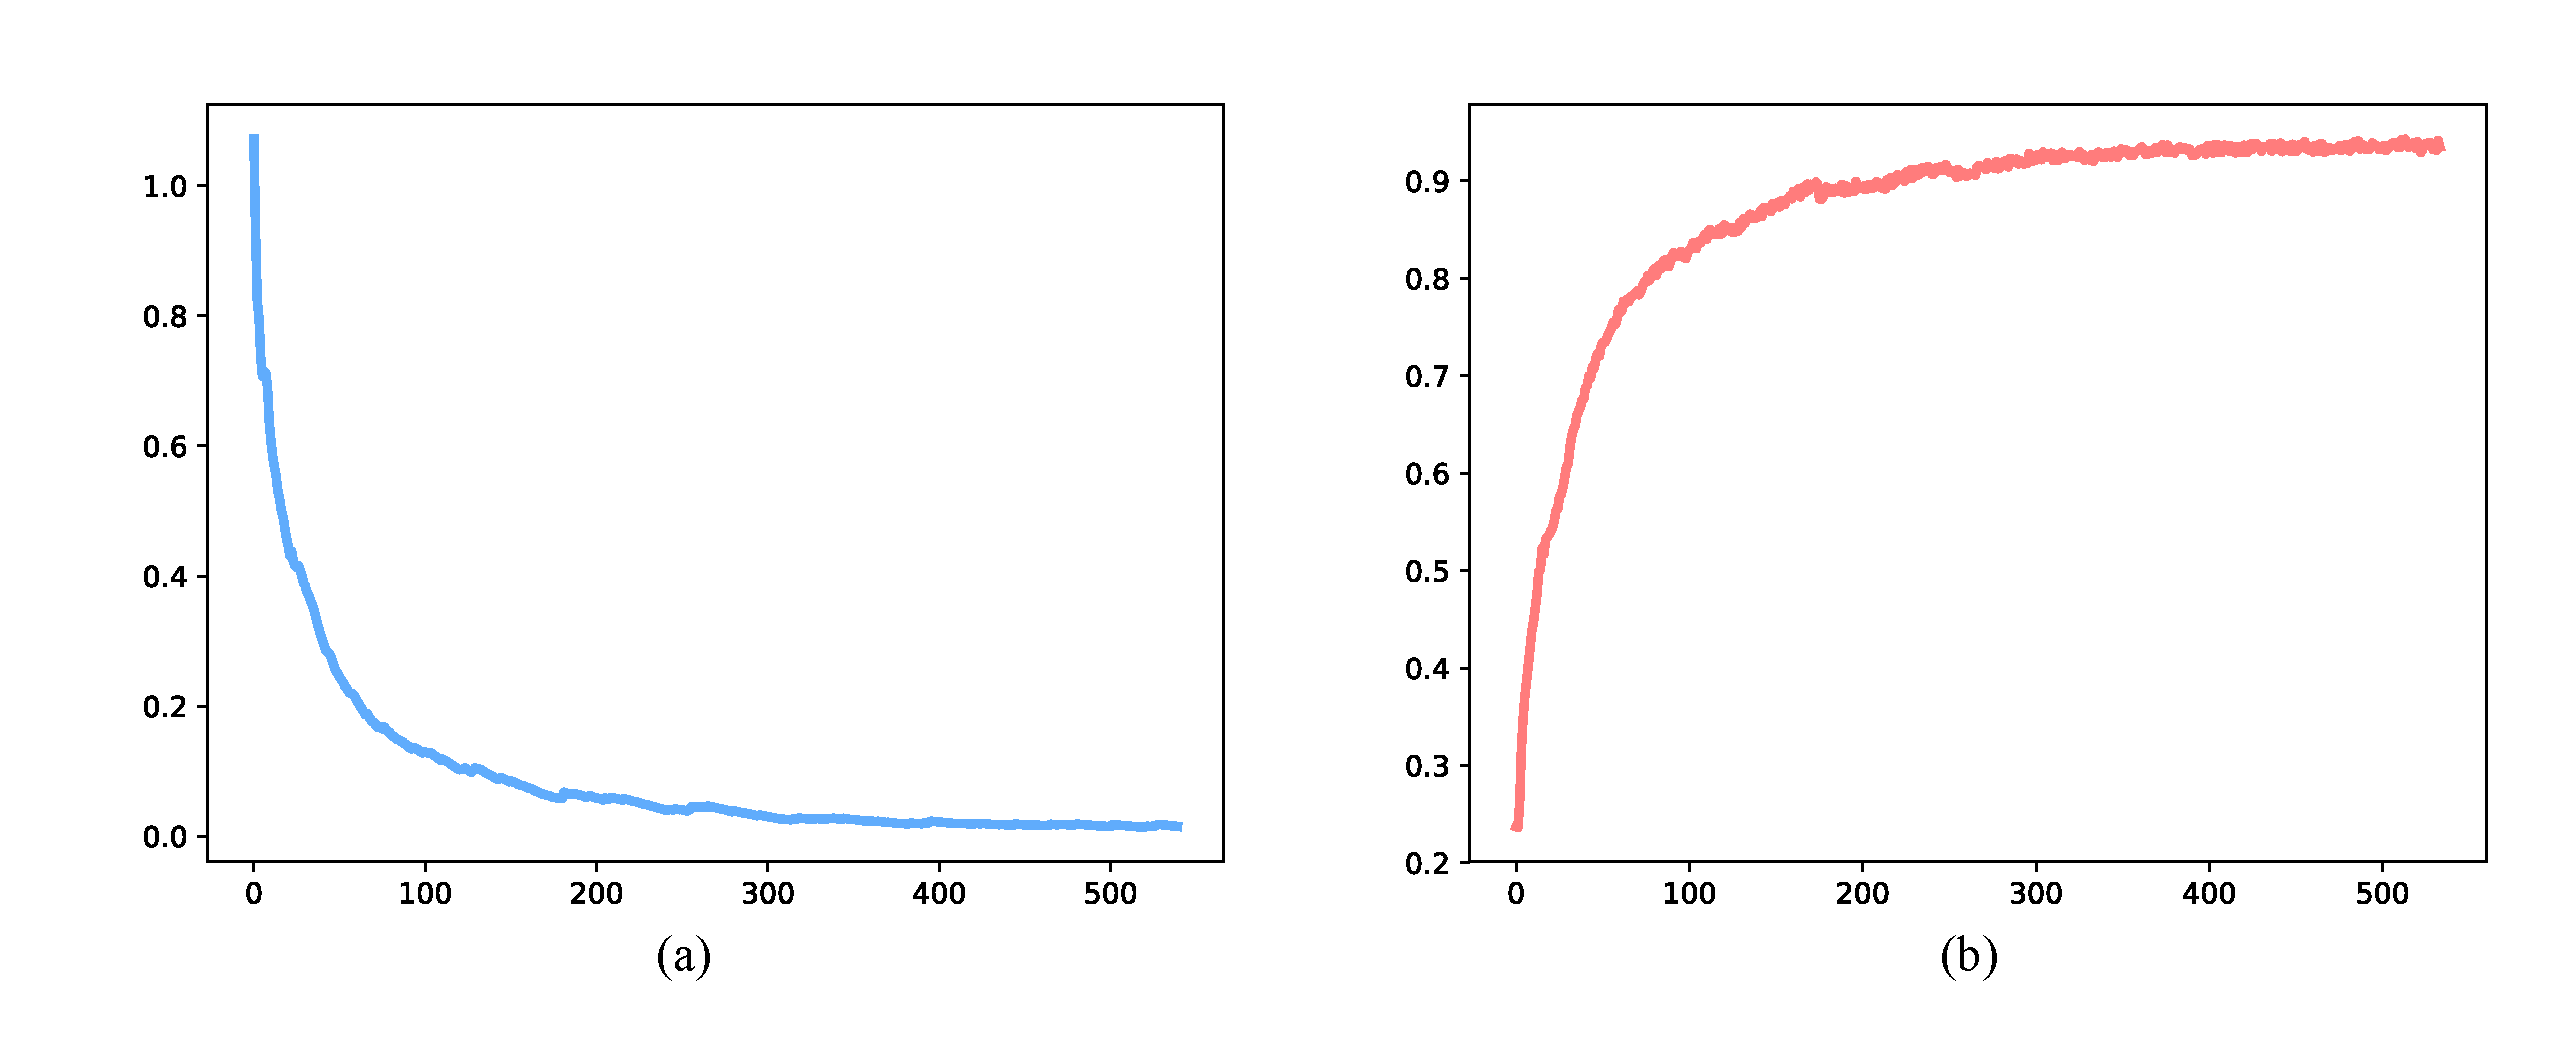
\includegraphics[width=15cm]{resx_acc.pdf}
\caption{(a): Loss and (b): accuracy curve of \textsf{ResNeXt} during the training process.}
\label{resxacc}
\end{figure}

}

\large{You are able to see the source code of this architecture in \textbf{Appendix. C.}}
%%%%%
\vspace{2mm}
\begin{center}
\large\textbf{Results} \\
\end{center}

\large{

\textbf{Fig. \ref{resxresults}} shows the scatter plot of predicted values for 4000 samples and the histogram of predicted values for them. We find that most scatters lie in the scale of 0.0-0.2, meaning that columnar cactus are absent in most images taken by UAVs in the testing set. Plus, most answers are explicit (\textit{i.$\ $e.}, the results are relatively sured), for almost all scatters are distributed in 0-0.2 and 0.8-1 (\textit{i.$\ $e.}, high confidence intervals).

}

\begin{figure}[h]
\centering
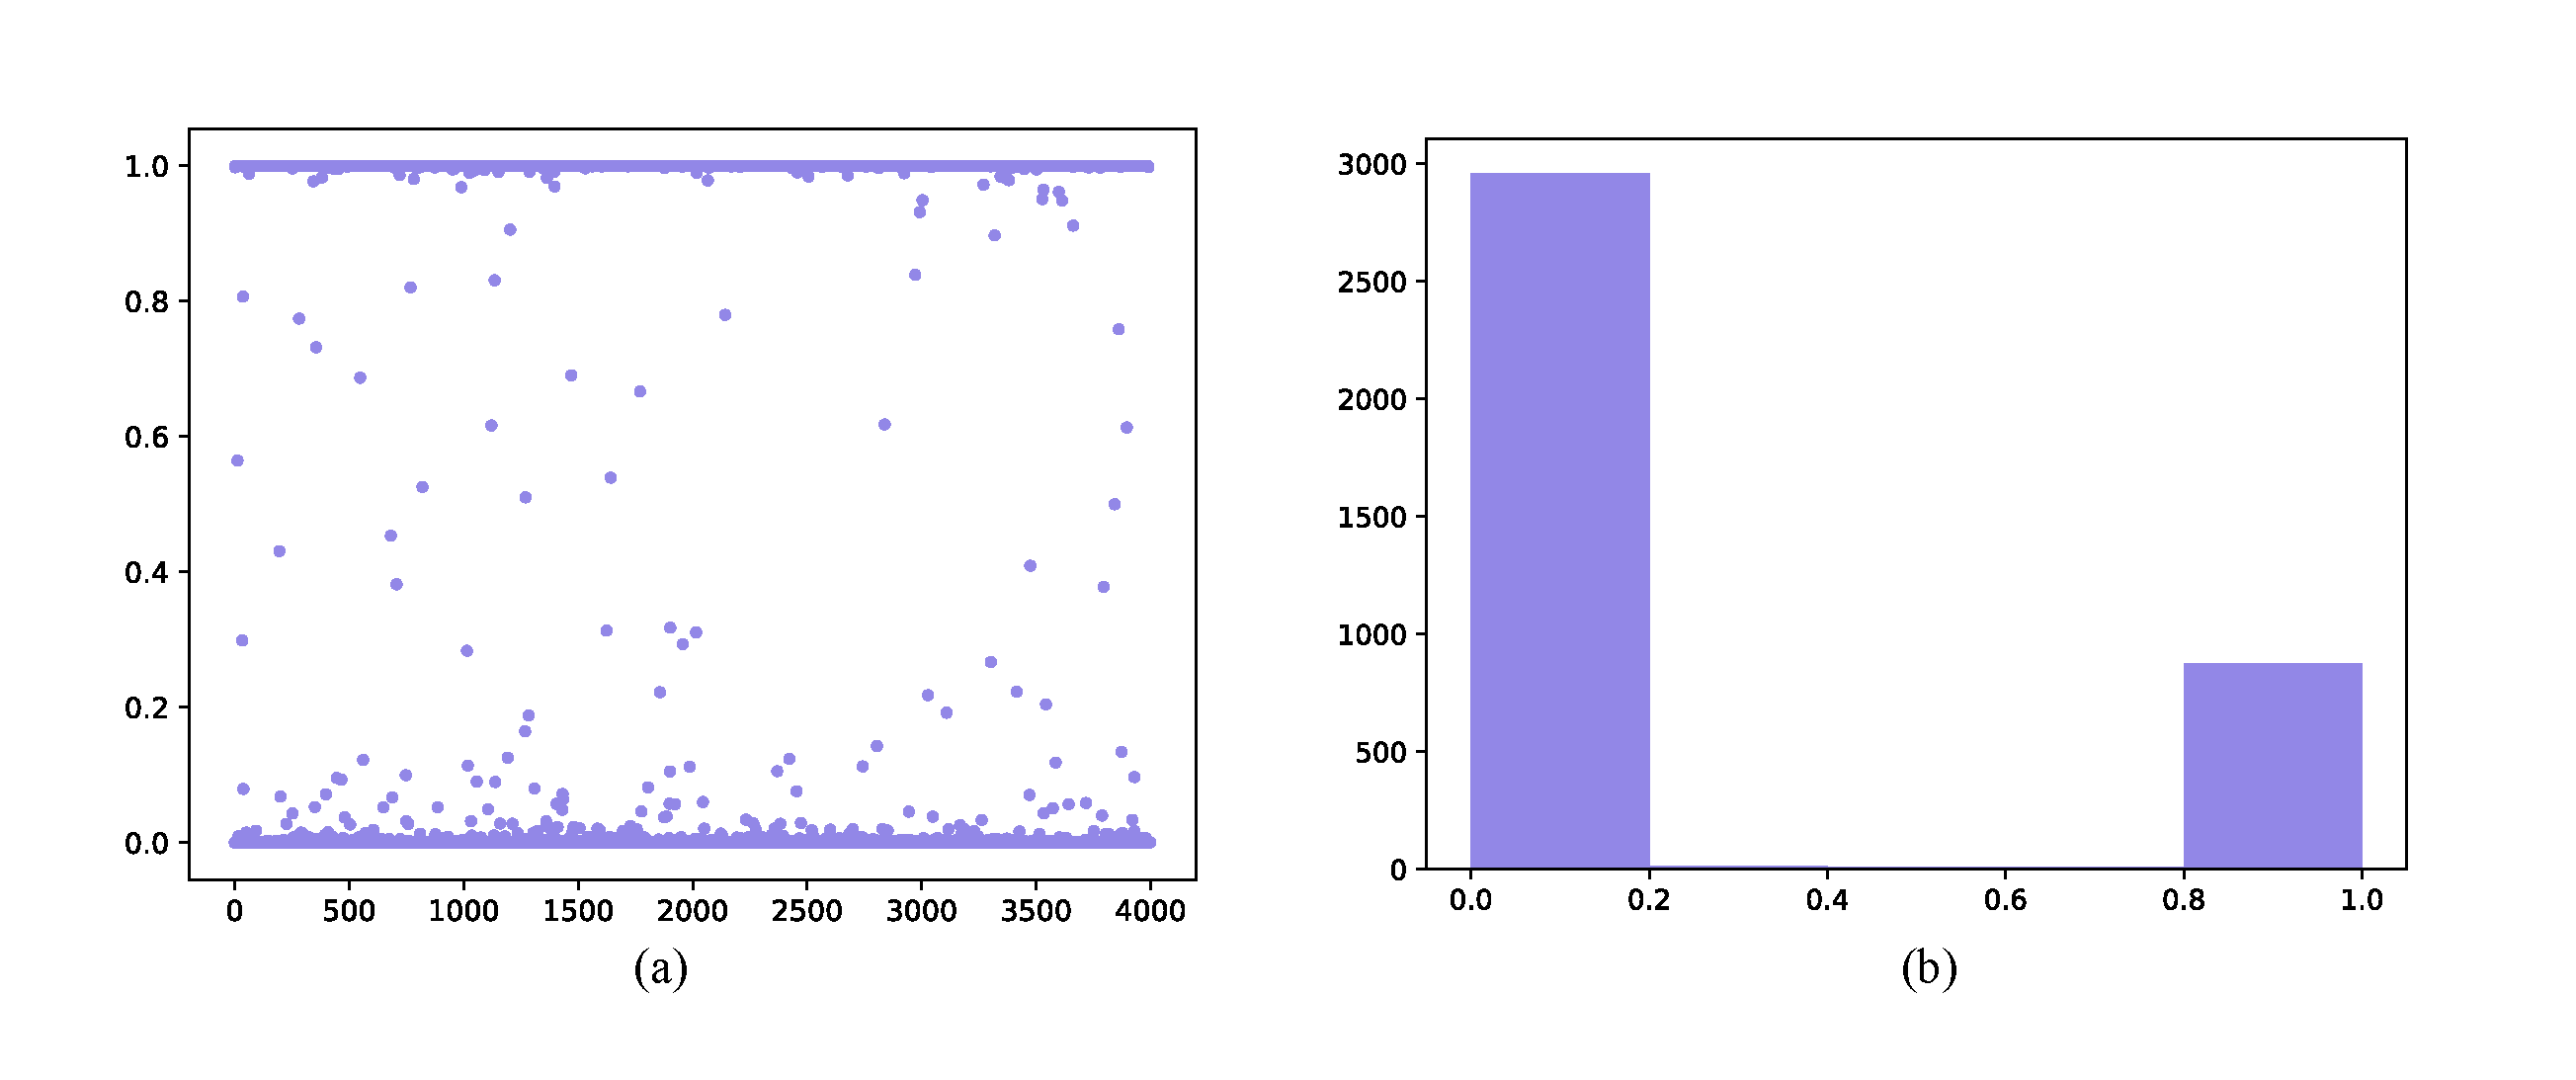
\includegraphics[width=15cm,height=6cm]{resx_best.pdf}
\caption{ (a): Prediction scatter and (b): prediction histogram of \textsf{ResNeXt}.}
\label{resxresults}
\end{figure}

%%%%%
\vspace{2mm}
\begin{center}
\large\textbf{Evaluation} \\
\end{center}
%resnext_50_1e-2_sgd_use-one-cycle_dofilp-flipvert
\large{
Our \textsf{ResNeXt} architecture has a up to \textbf{97.79\%} accuracy on the testing set when adopting the appropriate setting, (\textit{i.e.} 50 layer, 1e-1 learning rate, Adam optimizer, use one-cycle, and do nothing pre-processing). We also compare the impacts of parameters on the final score between different models as shown in \textbf{Fig. \ref{resxcompare}}. We find that pre-processing techniques like flipping images can not make the models more accurate, on the contrary, they even degrade the performance. Among the three models, \textsf{ResNeXt-50} perform the best and it's a rational measurement to exploit Adam optimizer in the models. Meanwhile, learning rate of 1e-1 is appropriate for training. The last sub-figure shows that one-cycle scheduler doesn't have huge effect on the overall performance. Note that all of the comparison is base on this baseline -- adopting flip techniques on \textsf{VGGNet-16} with a learning rate of 1e-2, using SGD optimizer and one-cycle scheduler.

\begin{figure}[h]
\centering
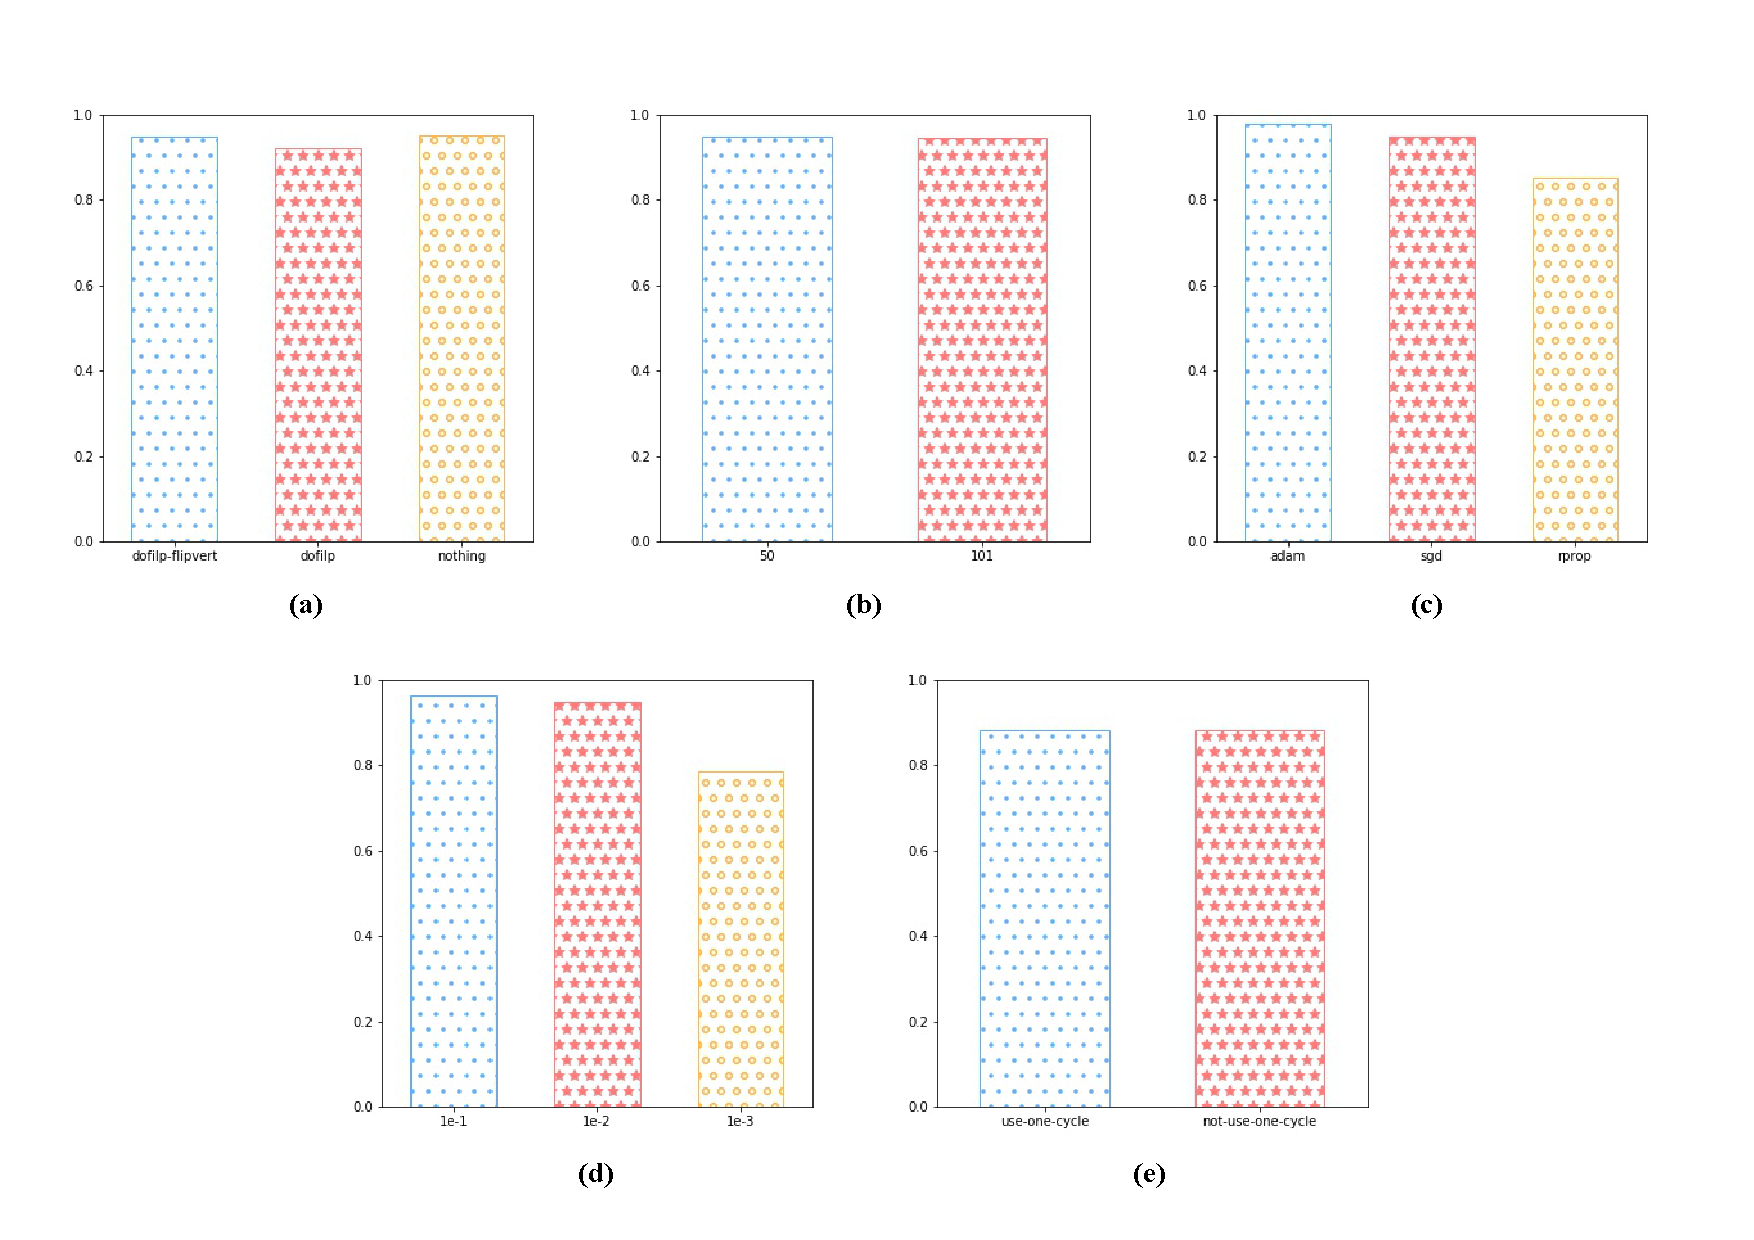
\includegraphics[width=15cm]{resX.pdf}
\caption{ Impacts of (a): pre-processing techniques, (b): the number of layer, (c): optimizer, (d) learning rate, and (e) scheduler between different models of \textsf{ResNeXt}.}
\label{resxcompare}
\end{figure}

}

%%% section VIII. Architecture Comparison
\vspace{5mm}
\begin{center}
\LARGE\textbf{VIII. Comparison and Impacts} \\
\end{center}

In this section, we first visualize the problem context using different architectures. Then, performance comparison is made among \textbf{5} architectures. Finally, we discuss the impacts of parameters on each architecture.

%%%%%
\vspace{2mm}
\begin{center}
\large\textbf{Visualization} \\
\end{center}

\large{
Shown in \textbf{Fig. \ref{cacuav5}}, the Mexico columnar cactus are circled in red. It's amazing that this networks can find out almost all cactus, which are hard to identify even with human-eye. 

\begin{figure}[h]
\centering
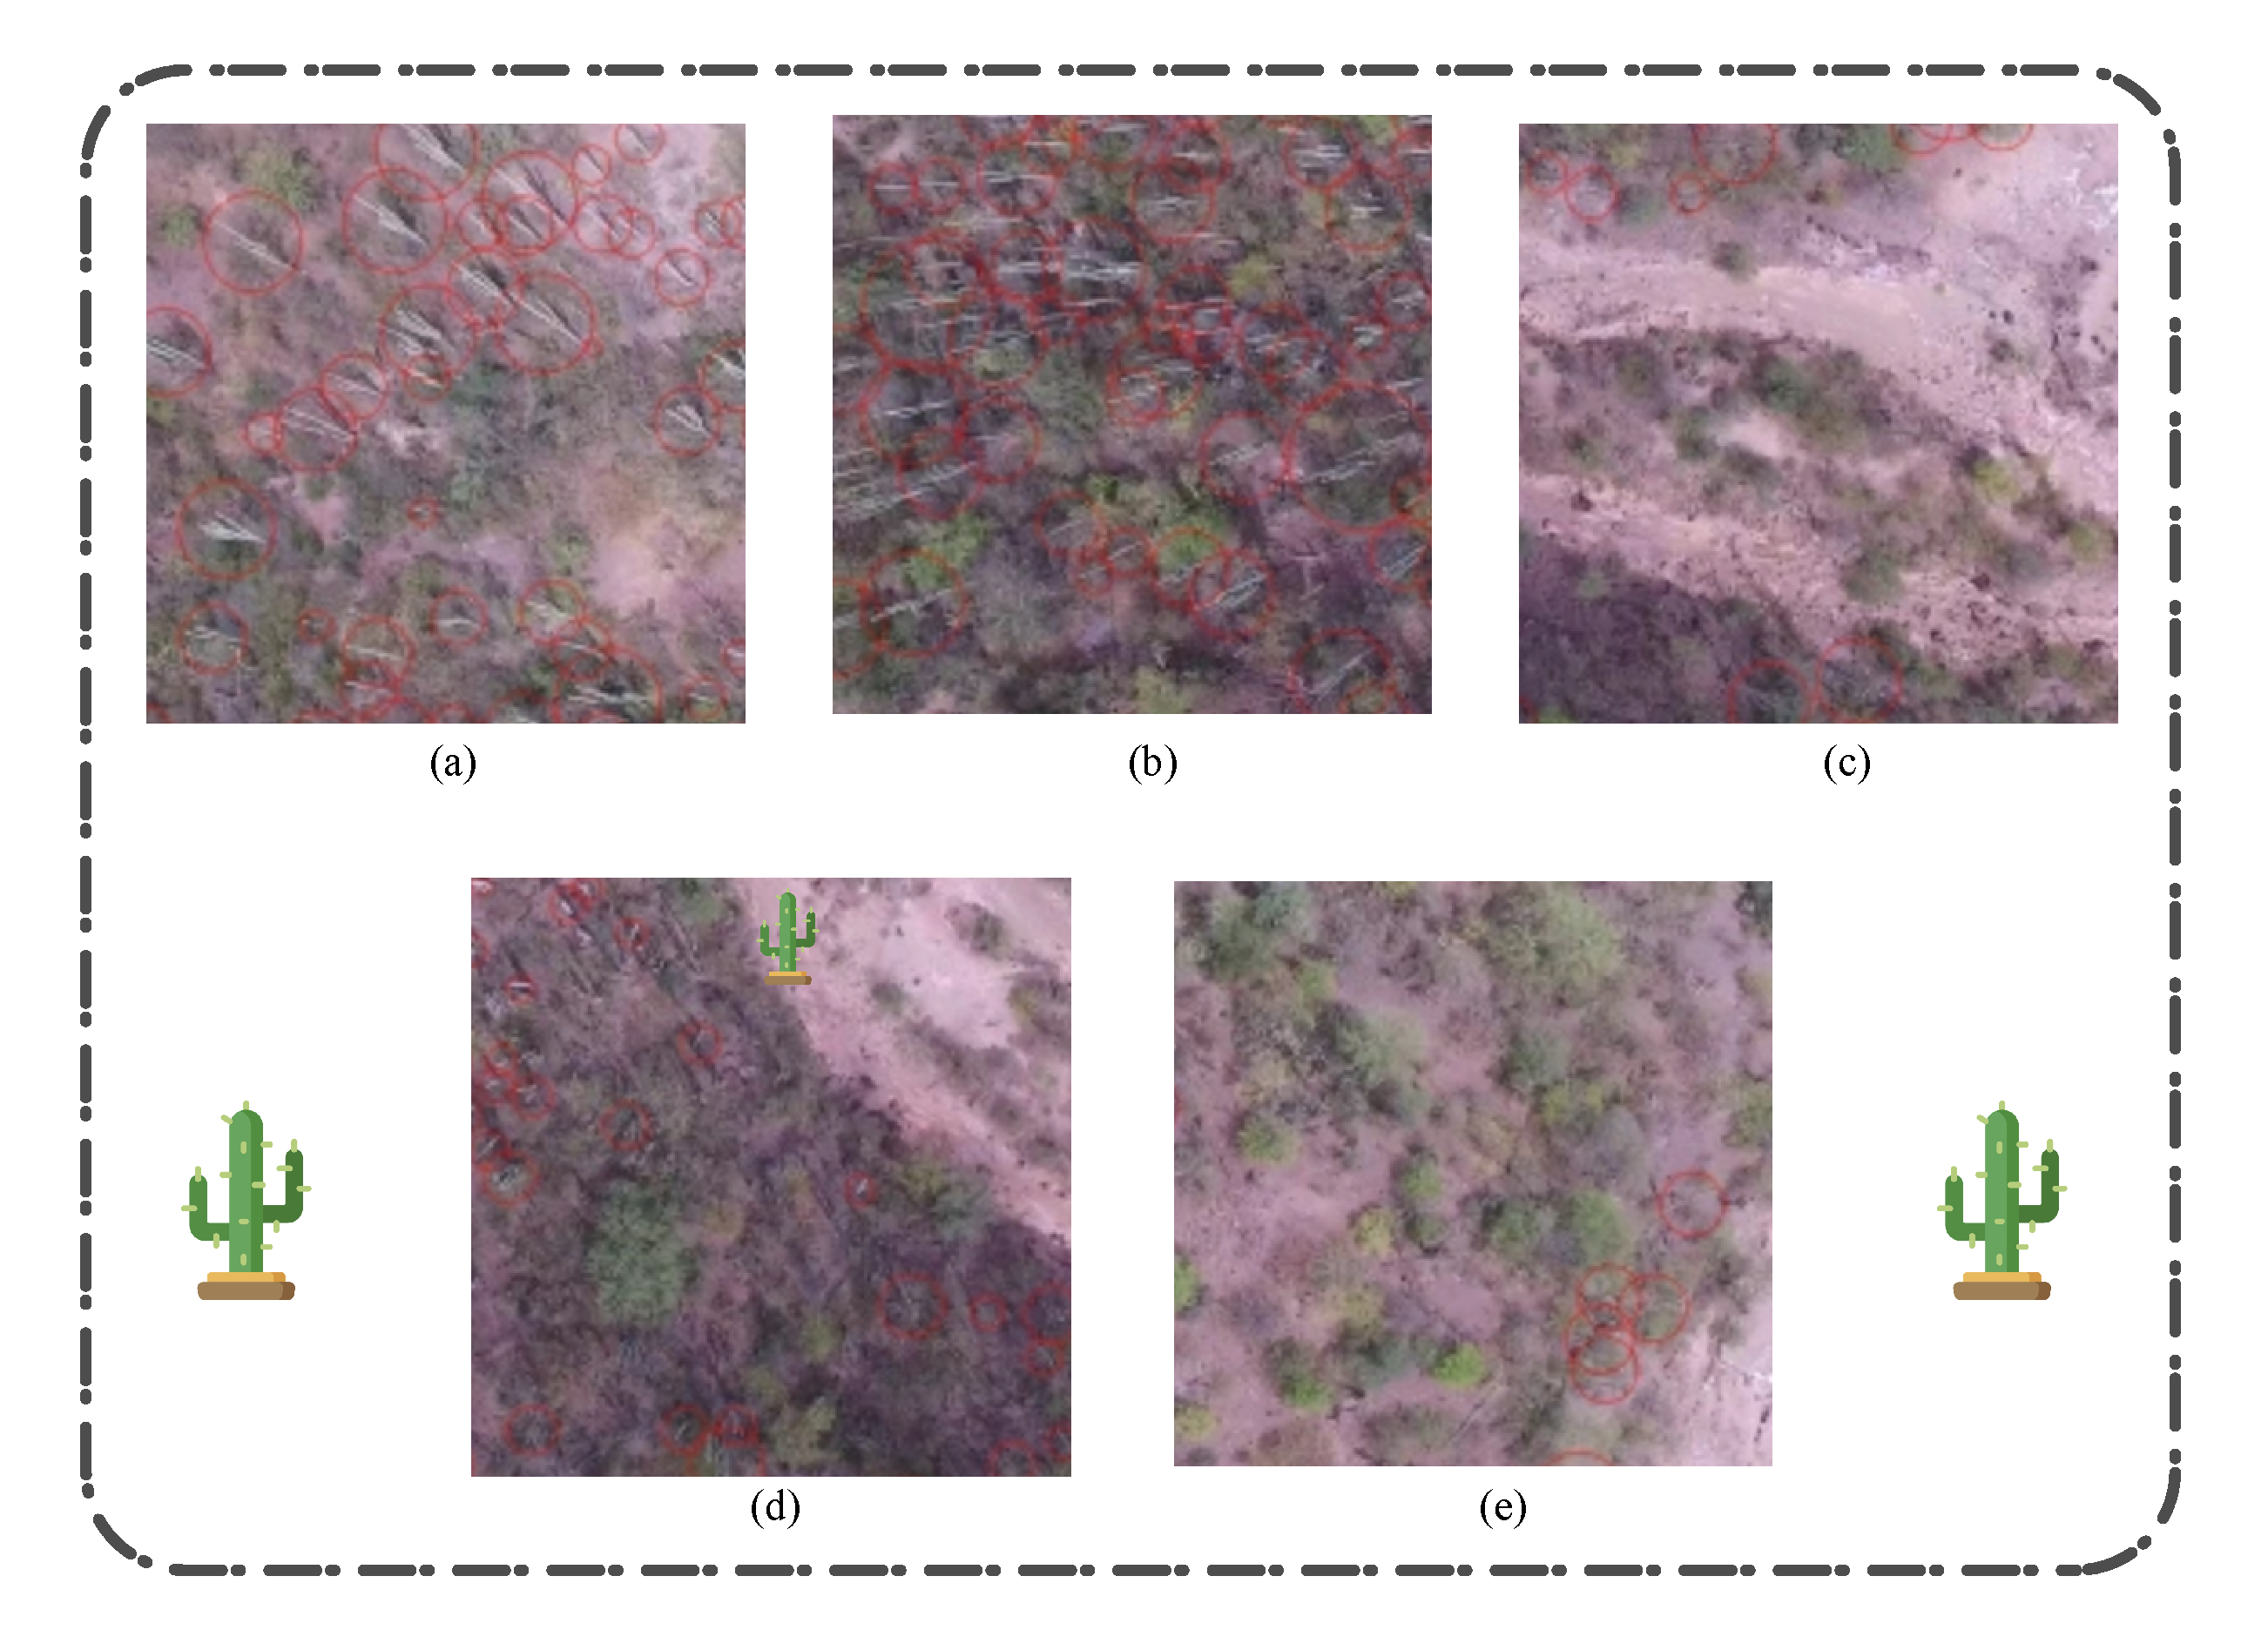
\includegraphics[width=15cm]{cacUAV5.pdf}
\caption{ Visualization by (a): \textsf{VGGNet}, (b): \textsf{ResNet}, (c): \textsf{SEResNet}, (d) \textsf{DenseNet}, and (e) \textsf{ResNeXt}.}
\label{cacuav5}
\end{figure}
}

%%%%%
\vspace{2mm}
\begin{center}
\large\textbf{Comparison} \\
\end{center}

\large{
To compare the performances of our architectures, we use \textbf{5} criteria to evaluate them. Comparison table is shown in \textbf{Table. \ref{comparetable}}.

%% tabletabletable
\begin{table*}[h]

\scriptsize

\centering

\caption{Comparison Table.}

\label{comparetable}

\begin{tabular}{ccccccccccc}
\\
\toprule

\multirow{2}{*}{Evaluation} && \multicolumn{2}{c}{Training set} &&&&& \multicolumn{2}{c}{Testing set} \\

\cmidrule(r){2-6}  \cmidrule(r){7-11}

\tiny{&   ROC   & F1  & Recall   & Pre   & Acc

&  ROC   & F1  & Recall   & Pre   & Acc} \\

\midrule

\textsf{VGGNet} \tiny{&9.99e-1 &9.90e-1 &9.87e-1 &9.93e-1  &9.85e-1 &9.98e-1 &9.35e-1 &9.93e-1 &8.84e-1  &9.66e-1}  \\

\textsf{ResNet}  \tiny{&1.00 &9.94e-1 &9.94e-1 &9.95e-1  &9.91e-1 &9.99e-1 &9.76e-1 &9.93e-1 &9.59e-1  &9.88e-1}  \\

\textsf{SEResNet}  \tiny{&9.97e-1 &9.86e-1 &9.83e-1 &9.89e-1  &9.79e-1    &9.95e-1 &9.21e-1 &9.76e-1 &8.72e-1  &9.58e-1}  \\

\textsf{DenseNet}  \tiny{&1.00 &9.97e-1 &9.97e-1 &9.98e-1  &9.96e-1 &1.00 &9.81e-1 &9.98e-1 &9.65e-1 &9.91e-1 }  \\

\textsf{ResNeXt}  \tiny{&1.00 &9.97e-1 &9.97e-1 &9.96e-1  &9.95e-1 &1.00 &9.73e-1 &9.97e-1 &9.50e-1 &9.86e-1}  \\

\bottomrule

\end{tabular}

\end{table*}

In this part, we exploit 5 criteria (\textit{i.e.}, ROC area, F1-measure, recall, precision, and accuracy) to evaluate each architecture. On both the training set and testing set, except the average accuracy, \textsf{DenseNet} always has an absolute advantage with respect to each column. This proves the stability of \textsf{DenseNet} network in various evaluating criteria.
}

%%%%%
\vspace{2mm}
\begin{center}
\large\textbf{Parameter Impacts} \\
\end{center}

\large{
As mentioned above, we use about \textbf{70} different setting to find the most suitable combination of each architecture. Besides, we try to figure out the marginal utility of each parameter in this part. The parameters we discuss here includes learning rate, data pre-processing techniques, the number of layer, and whether use one-cycle scheduler. The comparison results is shown in \textbf{Fig. \ref{impacttotal}}. Besides, the trend of loss and accuracy curve of architectures is also put together in \textbf{Fig. \ref{lossacctotal}} for a more detailed insight.

\begin{figure}[h]
\centering
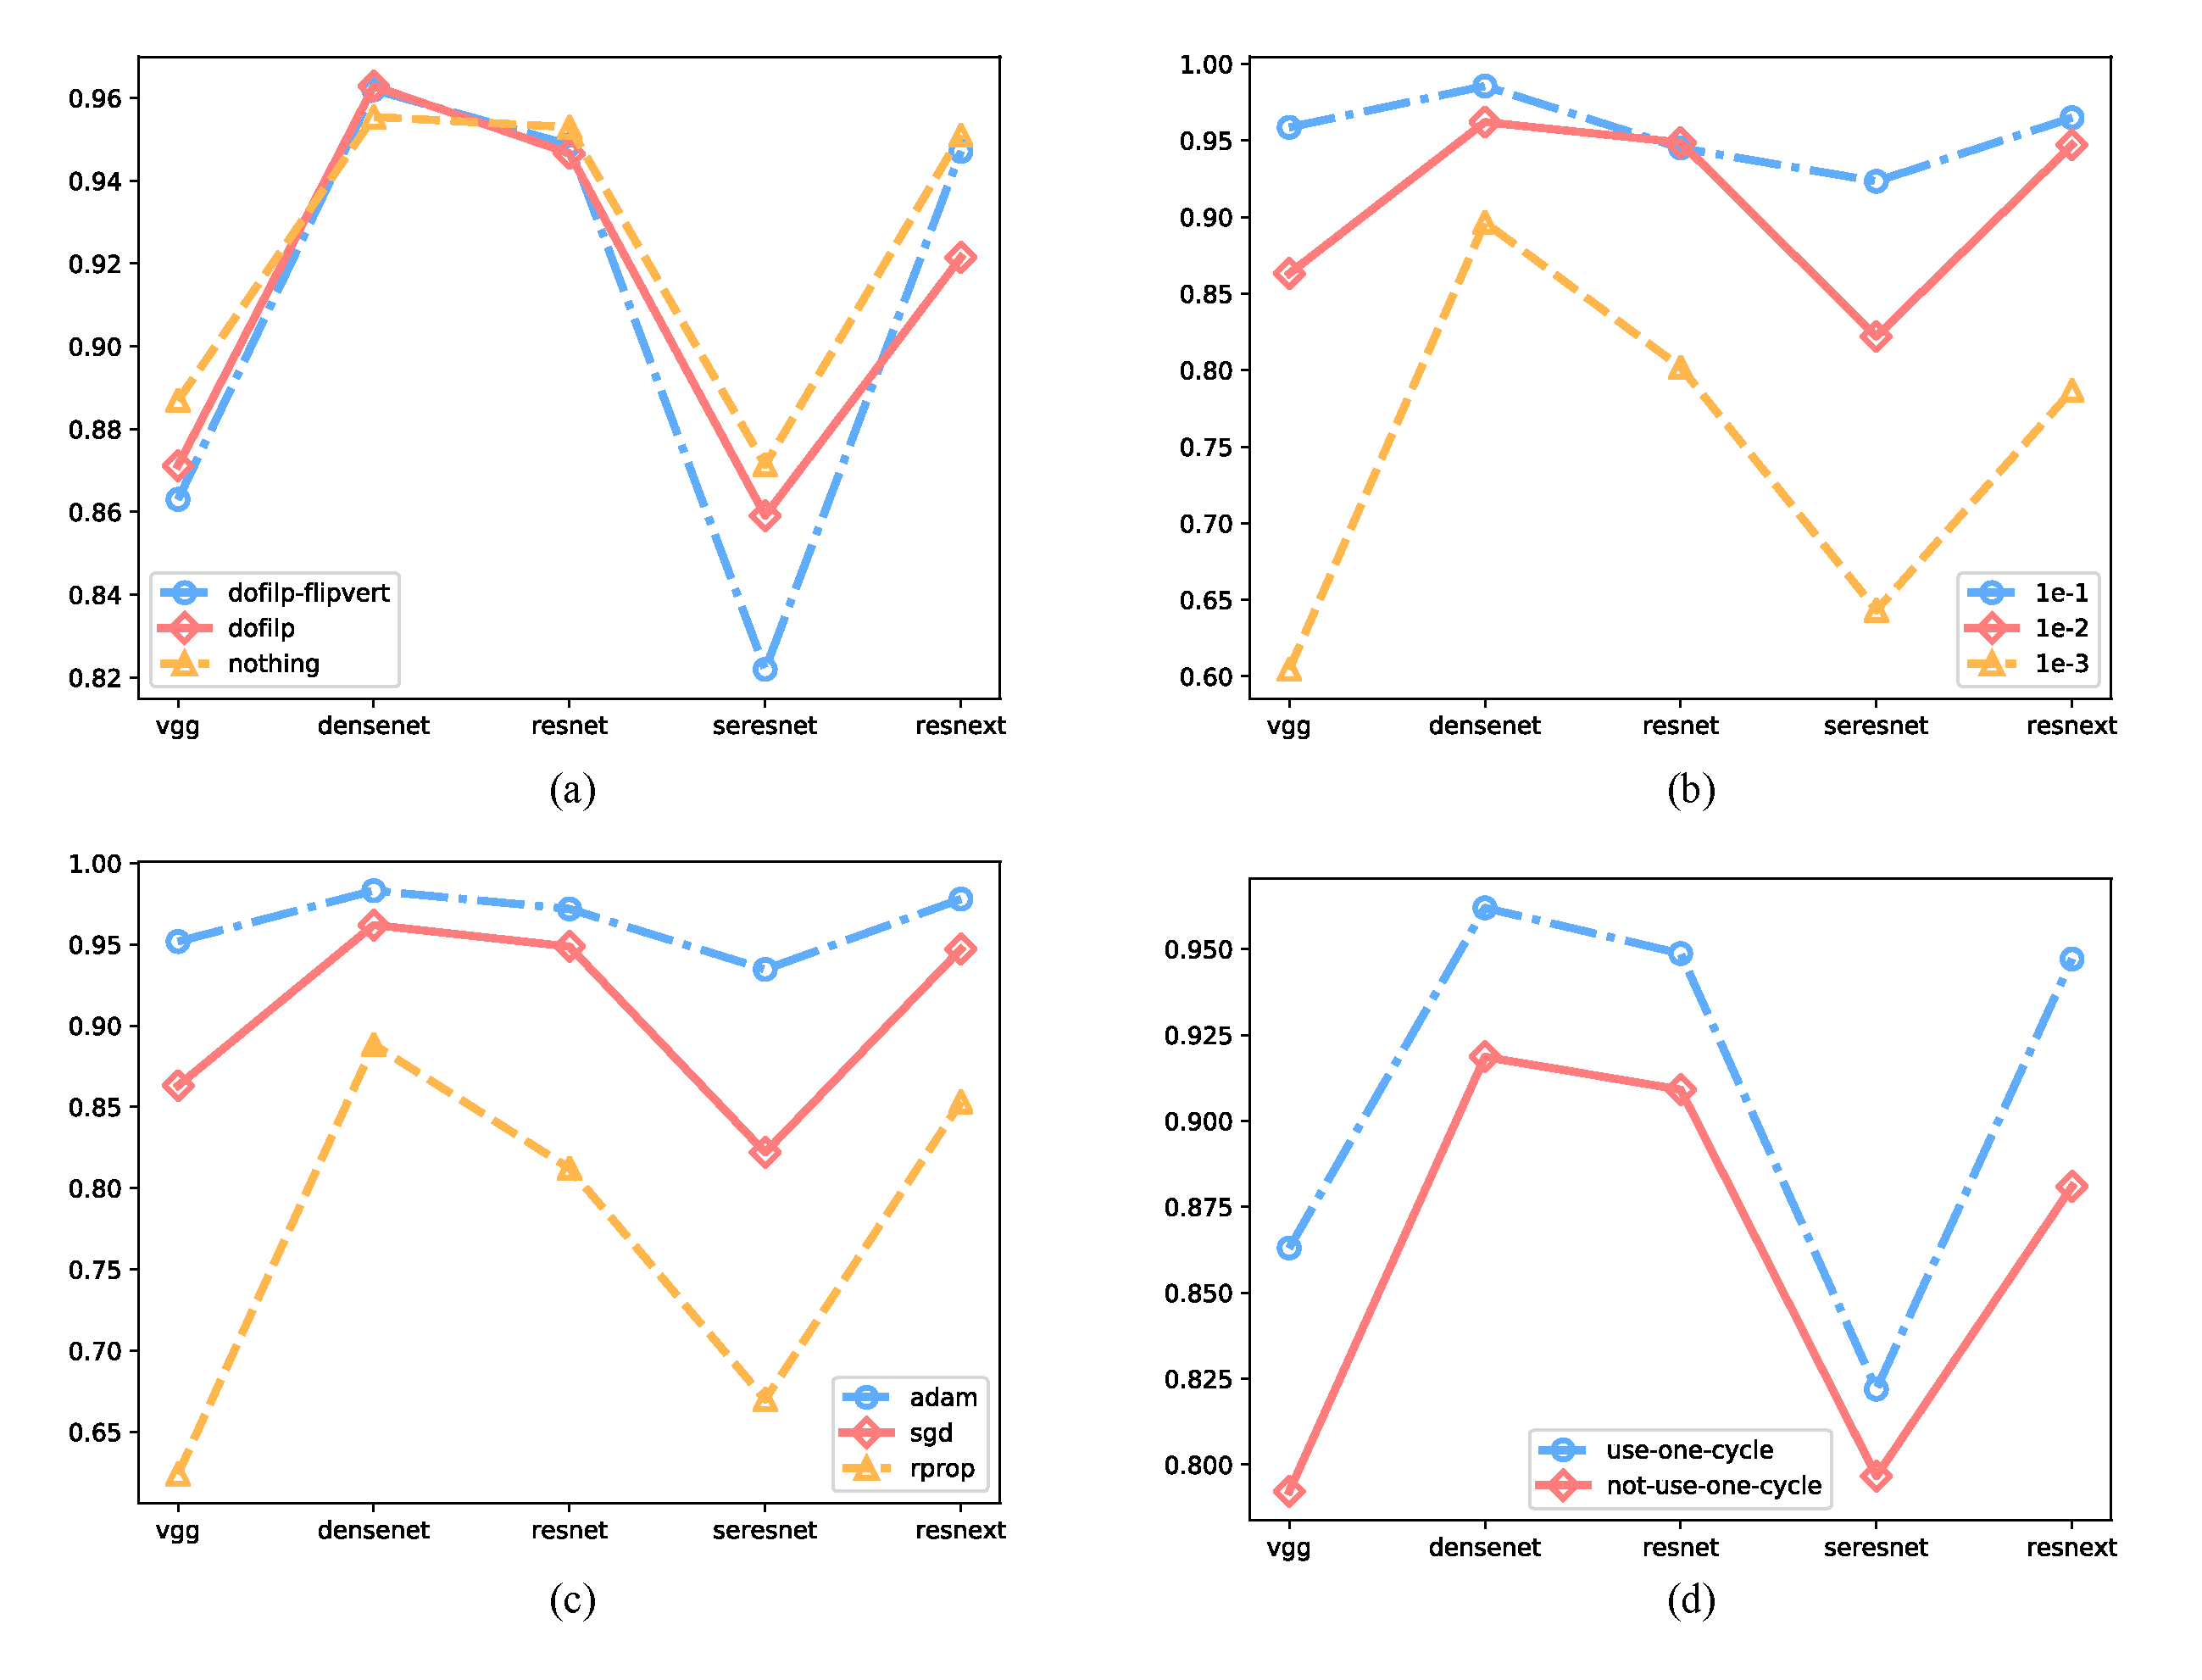
\includegraphics[width=15cm]{impact_total.pdf}
\caption{ Impacts of (a): pre-processing techniques, (b): learning rate, (c) optimizer, and (d) scheduler between different architectures.}
\label{impacttotal}
\end{figure}

We made a horizontal comparison between architectures. In \textbf{Fig. \ref{impacttotal}}, \textsf{DenseNet} and \textsf{ResNet} architectures are relatively stable under all circumstances, that is, have the least variance. This proves that the parameters have little influence on these architectures. While, \textsf{DenseNet} has a average better performance over \textsf{ResNet}, which shows that it is the most suitable measurement for this problem. As the enhancement of \textsf{ResNet}, \textsf{SEResNet} does not reach the expectation as \textsf{ResNeXt} and \textsf{DenseNet}, and it seems to be the worst among these architectures. 

A longitudinal comparison is also made. See that data pre-processing techniques have the least influences on the models. On the contrary, learning rate variance is the most important contributor to the score in this situation. In addition, Adam optimizer always gets the highest score and it is pretty stable. Lastly, the one-cycle scheduler has a good effect on improving the performance.

We carefully think about these phenomenons and conclude several reasons. First, as there are many data pre-processing techniques, we only use a limited number of them. Thus, it would be exaggerate to underestimate the power of these techniques. Second, although the learning rate variance seems to contribute to models a lot now, this maybe change if we narrow the interval. In other words, 1e-1 $\gg$ 1e-2 $\gg$ 1e-3. Therefore, this comparison just view from a micro-viewpoint and is not generalized for all situations. From this perspective, it would be arbitrary to draw a too absolute conclusion.

\begin{figure}[h]
\centering
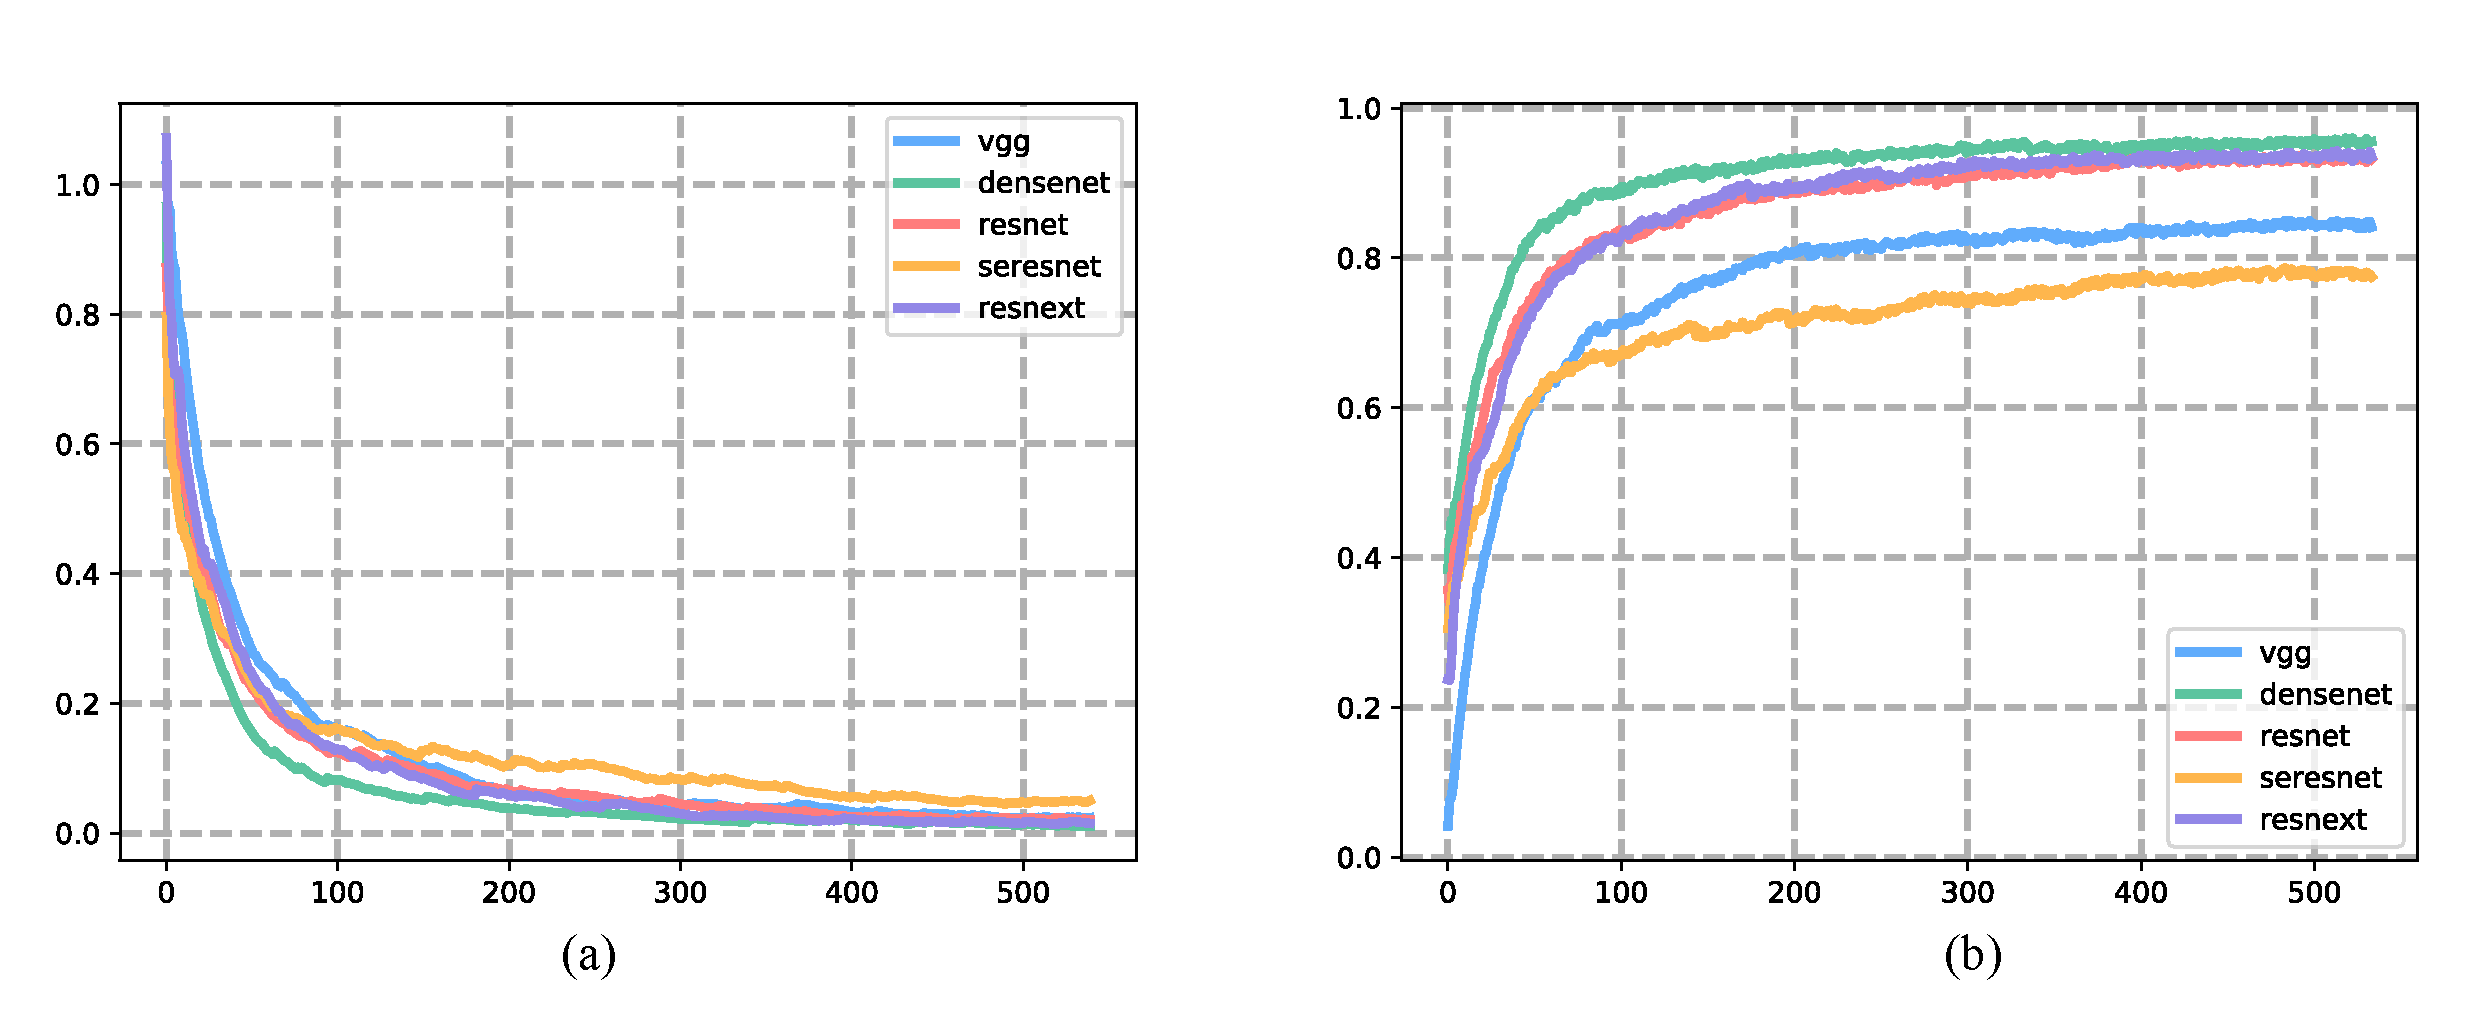
\includegraphics[width=15cm]{loss_total.pdf}
\caption{ (a): Loss and (b):accuracy curve of five architectures during training.}
\label{lossacctotal}
\end{figure}

\textbf{Fig. \ref{lossacctotal}} illustrates the curve of loss and accuracy during training. The training rate of \textsf{DenseNet} is always way ahead, which shows its advancement. Moreover, we have some interesting observations. \textsf{VGGNet} is one full of potential: it seems to have the lowest training rate in the early stage, but gradually comes up with the large forces. \textsf{SEResNet} falls behind from the $60^{th}$ epoch, though it's training rate is pretty fast in the early. Other architectures are fairly regular and have no much surprise.

}
\clearpage
%%
\vspace{15mm}
\begin{center}
\LARGE\textbf{IX. Conclusion} \\
\end{center}
\vspace{2mm}

\large{This is a scientific report for \href{https://www.kaggle.com/c/aerial-cactus-identification/overview}{Kaggle Competition: \texttt{Aerial Cactus Identification.}} In this competition, to recognize the vegetation inside the protected areas of Mexico, we are aiming to build models to identify columnar cactus from aerial photos. We build \textbf{14} models under \textbf{5} architectures, and try about \textbf{70} different parameter settings to get the most suitable parameter combination (see overview in \textbf{Fig.} \ref{overview}). We find that \textsf{DenseNet-161} does the most accurate cactus identification job and \textbf{we get grade 0.9997\/1.0 on Kaggle}. Moreover, we make horizontal comparison between models as well as compare architectures longitudinally. This elaborated work provides us an overall understanding of the architectures, helping us to figure out the parameter impacts at the same time. }


%%
\vspace{1.5cm}
\begin{center}
\LARGE\textbf{X. Acknowledgement} \\
\end{center}
\vspace{.5mm}

\begin{itemize} \item{First and foremost, we would like to show my deepest gratitude to my teacher, professor \textbf{Liang}, who has provided us with valuable theoretical guidance of deep learning. Without his enlightening instruction, impressive kindness and patience, we could never have completed our projects. His keen and vigorous academic observation enlightens us in this thesis and our future study.}
\item{My sincere appreciation also goes to our \textbf{teammates}. We got along in harmony and had a good time. They offered us valuable advice which is pretty beneficial. All of these make this experience meaningful.}
\end{itemize}

\clearpage
%%
\vspace{5mm}
\begin{center}
\LARGE\textbf{XI. Appendices} \\
\end{center}

\vspace{5mm}
\begin{center}
\large\textbf{A. Competition} \\
\end{center}

\large{
\begin{itemize}
    \item \textbf{Competition}: \underline{\href{https://www.kaggle.com/c/aerial-cactus-identification/overview}{Aerial Cactus Identification (\emph{Playground})}}
    \item \textbf{Time Line}: The competition will conclude July 8, 2019 at 11:59 PM UTC. 
    \item \textbf{Dataset}: $32 \times 32$ thumbnail columnar cactus images.
    \item \textbf{Target}: Creating a classifier to predict the probability of containing cactus.
\end{itemize}
}

\vspace{5mm}
\begin{center}
\large\textbf{B. Submission Pages} \\
\end{center}


\vspace{2mm}
\large{
Submission pages of our 5 models are listed as follows.
\begin{itemize}
    \item \textsf{VGG}:  \underline{\href{https://www.kaggle.com/albertsheldon/test-m2?scriptVersionId=16988178}{https://www.kaggle.com/albertsheldon/test-m2?scriptVersionId=16988178}}
    \item \textsf{ResNet}: \underline{\href{https://www.kaggle.com/albertsheldon/test-resnet}{https://www.kaggle.com/albertsheldon/test-resnet}}
    \item \textsf{SEResNet}: \underline{\href{https://www.kaggle.com/albertsheldon/test-m2}{https://www.kaggle.com/albertsheldon/test-m2}}
    \item \textsf{DenseNet}: \underline{\href{https://www.kaggle.com/albertsheldon/test-m1?scriptVersionId=16987923}{https://www.kaggle.com/albertsheldon/test-m1?scriptVersionId=16987923}}
    \item \textsf{ResNeXt}: \underline{\href{https://www.kaggle.com/albertsheldon/test-m1}{https://www.kaggle.com/albertsheldon/test-m1}}
\end{itemize}
}

\vspace{5mm}
\begin{center}
\large\textbf{C. Source Code} \\
\end{center}

\large{All of the code has update to our GitHub repository, click \href{https://github.com/LovelyBuggies/Jupyter_DeepLearning_Homework/tree/master/Identify-Cactus/project/src}{\underline{this link}} to view all of the soure code.}

\vspace{5mm}

\noindent \normalsize \textbf{1) \textsf{VGGNet}: vgg.py} \small

\noindent \HRule

\lstinputlisting[language=python]{./vgg.py}

\noindent \HRule

\vspace{1.5cm}

\noindent \normalsize \textbf{2) \textsf{ResNet} \& \textsf{ResNeXt}: res.py} \small

\noindent \HRule

\lstinputlisting[language=python]{./resnet.py}

\noindent \HRule

\vspace{1.5cm}

\noindent \normalsize \textbf{3) \textsf{DenseNet}: densenet.py} \small

\noindent \HRule

\lstinputlisting[language=python]{./densenet.py} 

\noindent \HRule

\vspace{1.5cm}

\noindent \normalsize \textbf{4) \textsf{SEResNet}: se\_resnet.py} \small

\noindent \HRule

\lstinputlisting[language=python]{./se_resnet.py} 

\noindent \HRule

\vspace{1.5cm}

\noindent \normalsize \textbf{5) \textsf{Comparison}: code2.py} \small

\noindent \HRule

\lstinputlisting[language=python]{./code2.py} 

\noindent \HRule

\vspace{1.5cm}

\noindent \normalsize \textbf{6) \textsf{Requirements}: requirements.txt} \small

\noindent \HRule

\lstinputlisting[language=python]{./requirements.txt} 

\noindent \HRule

\vspace{2cm}


\end{document}
